\documentclass[xcolor=svgnames]{beamer}
\usetheme[
    %%% options passed to the outer theme
    %    hidetitle,           % hide the (short) title in the sidebar
    %    hideauthor,          % hide the (short) author in the sidebar
    %    hideinstitute,       % hide the (short) institute in the bottom of the sidebar
    %    shownavsym,          % show the navigation symbols
         width=1.5cm,         % width of the sidebar (default is 2 cm)
    %    hideothersubsections,% hide all subsections but the subsections in the current section
    %    hideallsubsections,  % hide all subsections
         left                 % right of left position of sidebar (default is right)
    %%% options passed to the color theme
        lightheaderbg         % use a light header background
  ]{AAUsidebar}

% #### graphics and schemes
\usepackage{graphicx}
\graphicspath{{img/}}
\usepackage{tikz}
\usetikzlibrary{                          % TikZ libraries
                scopes,                   % .
                shapes,                   % .
                arrows,                   % .
                through,                  % .
                calc,                     % .
                intersections,            % .
                spy,                      % .
                matrix,                   % .
                chains,                   % .
                decorations.pathreplacing,% .
                decorations.pathmorphing, % .
                decorations.markings}     % .

\usepackage{pgfplots}                     % TikZ plots
\usepackage{pgfplotstable}                % TikZ tables from CSV
\pgfplotsset{compat=1.3}                  % activates \xilabel shift` for pgfplots
\usepackage{array}
\usepackage{listings}
\usepackage{ccicons}
\usepackage{tcolorbox}
\usepackage{listings}                     % code
\usepackage{adjustbox}                    % code
\usepackage{eurosym}                      % euro symbol
\usepackage{attrib}

% #### colors
\usepackage{xcolor}                       % common color names
\usepackage{colortbl}                     % common color names

% #### layouts
\usepackage{multicol}
\usepackage[textfont=footnotesize,bf]{caption}
\usepackage{subfig}

% #### math
\usepackage{siunitx}

% #### fonts
\usepackage[utf8]{inputenc}
\usepackage[italian]{babel}
\usepackage[T1]{fontenc}
\usepackage{cmbright}
\usepackage{soul} %slanted text
\usepackage{hyperref}
\urlstyle{same}
\hypersetup{pdfauthor={Francesco de Virgilio},pdftitle={Geostatistica con GIS open source:\\gli insediamenti neolitici del Tavoliere}}

% #### tables
\usepackage{booktabs}			          % migliora la qualità delle tabelle
\usepackage{tabularx}			          % colonne a spaziatura fissa delle tabelle
\newcommand{\otoprule}                    % better top rule horizontal line
    {\midrule[\heavyrulewidth]}           % .

% #### mainmatter
\title[Geostatistica con GIS open source]{Geostatistica con GIS open source}
\subtitle{Gli insediamenti neolitici del Tavoliere\\{\tiny Tesi di laurea triennale in Geofisica applicata}}
\author[Francesco \mbox{de Virgilio}]{
    Francesco de Virgilio\\\vspace{0.05\textwidth}
    {\scriptsize
        Relatore: Ch.mo Prof. Marcello Ciminale\\
        ~~Correlatrice: dott.ssa Mariangela Noviello
    }
}
\date{}

% ### title page logo
\pgfdeclareimage[height=1.5cm]{titlepagelogo}{AAUgraphics/uniba} % placed on the title page
\titlegraphic{% is placed on the bottom of the title page
    \pgfuseimage{titlepagelogo}\\\vspace{-0.02\textwidth}
    {\tiny Dipartimento di Scienze della Terra e Geoambientali\\\vspace{-0.02\textwidth}
     Università degli Studi di Bari ``Aldo Moro''
    }
}

\begin{document}
    {\aauwavesbg%
        \begin{frame}[plain,noframenumbering]
            \titlepage
        \end{frame}
    }

    %\begin{frame}{Tirocinio}
        %\begin{columns}[c]
            %\column{0.48\textwidth}
            %\centering
            %\begin{figure}
                %\centering
                %
\includegraphics[width=0.5\textwidth]{AAUgraphics/uniba}
            %\end{figure}
            %\vspace{-0.2\textwidth}
            %Dip. di Scienze della Terra e Geoambientali\\
            %Università di Bari ``Aldo Moro''
            %\column{0.48\textwidth}
            %\centering
            %\begin{figure}
                %\centering
                %
\includegraphics[width=0.5\textwidth]{img/logo}
            %\end{figure}
            %\vspace{-0.1\textwidth}
            %L.--P. Archaeology\\
            %Londra, Regno Unito
        %\end{columns}
    %\end{frame}

    \begin{frame}{Insediamenti neolitici}
        \centering
        \begin{tikzpicture}
            \node[anchor=south west,inner sep=0] at (0,0) {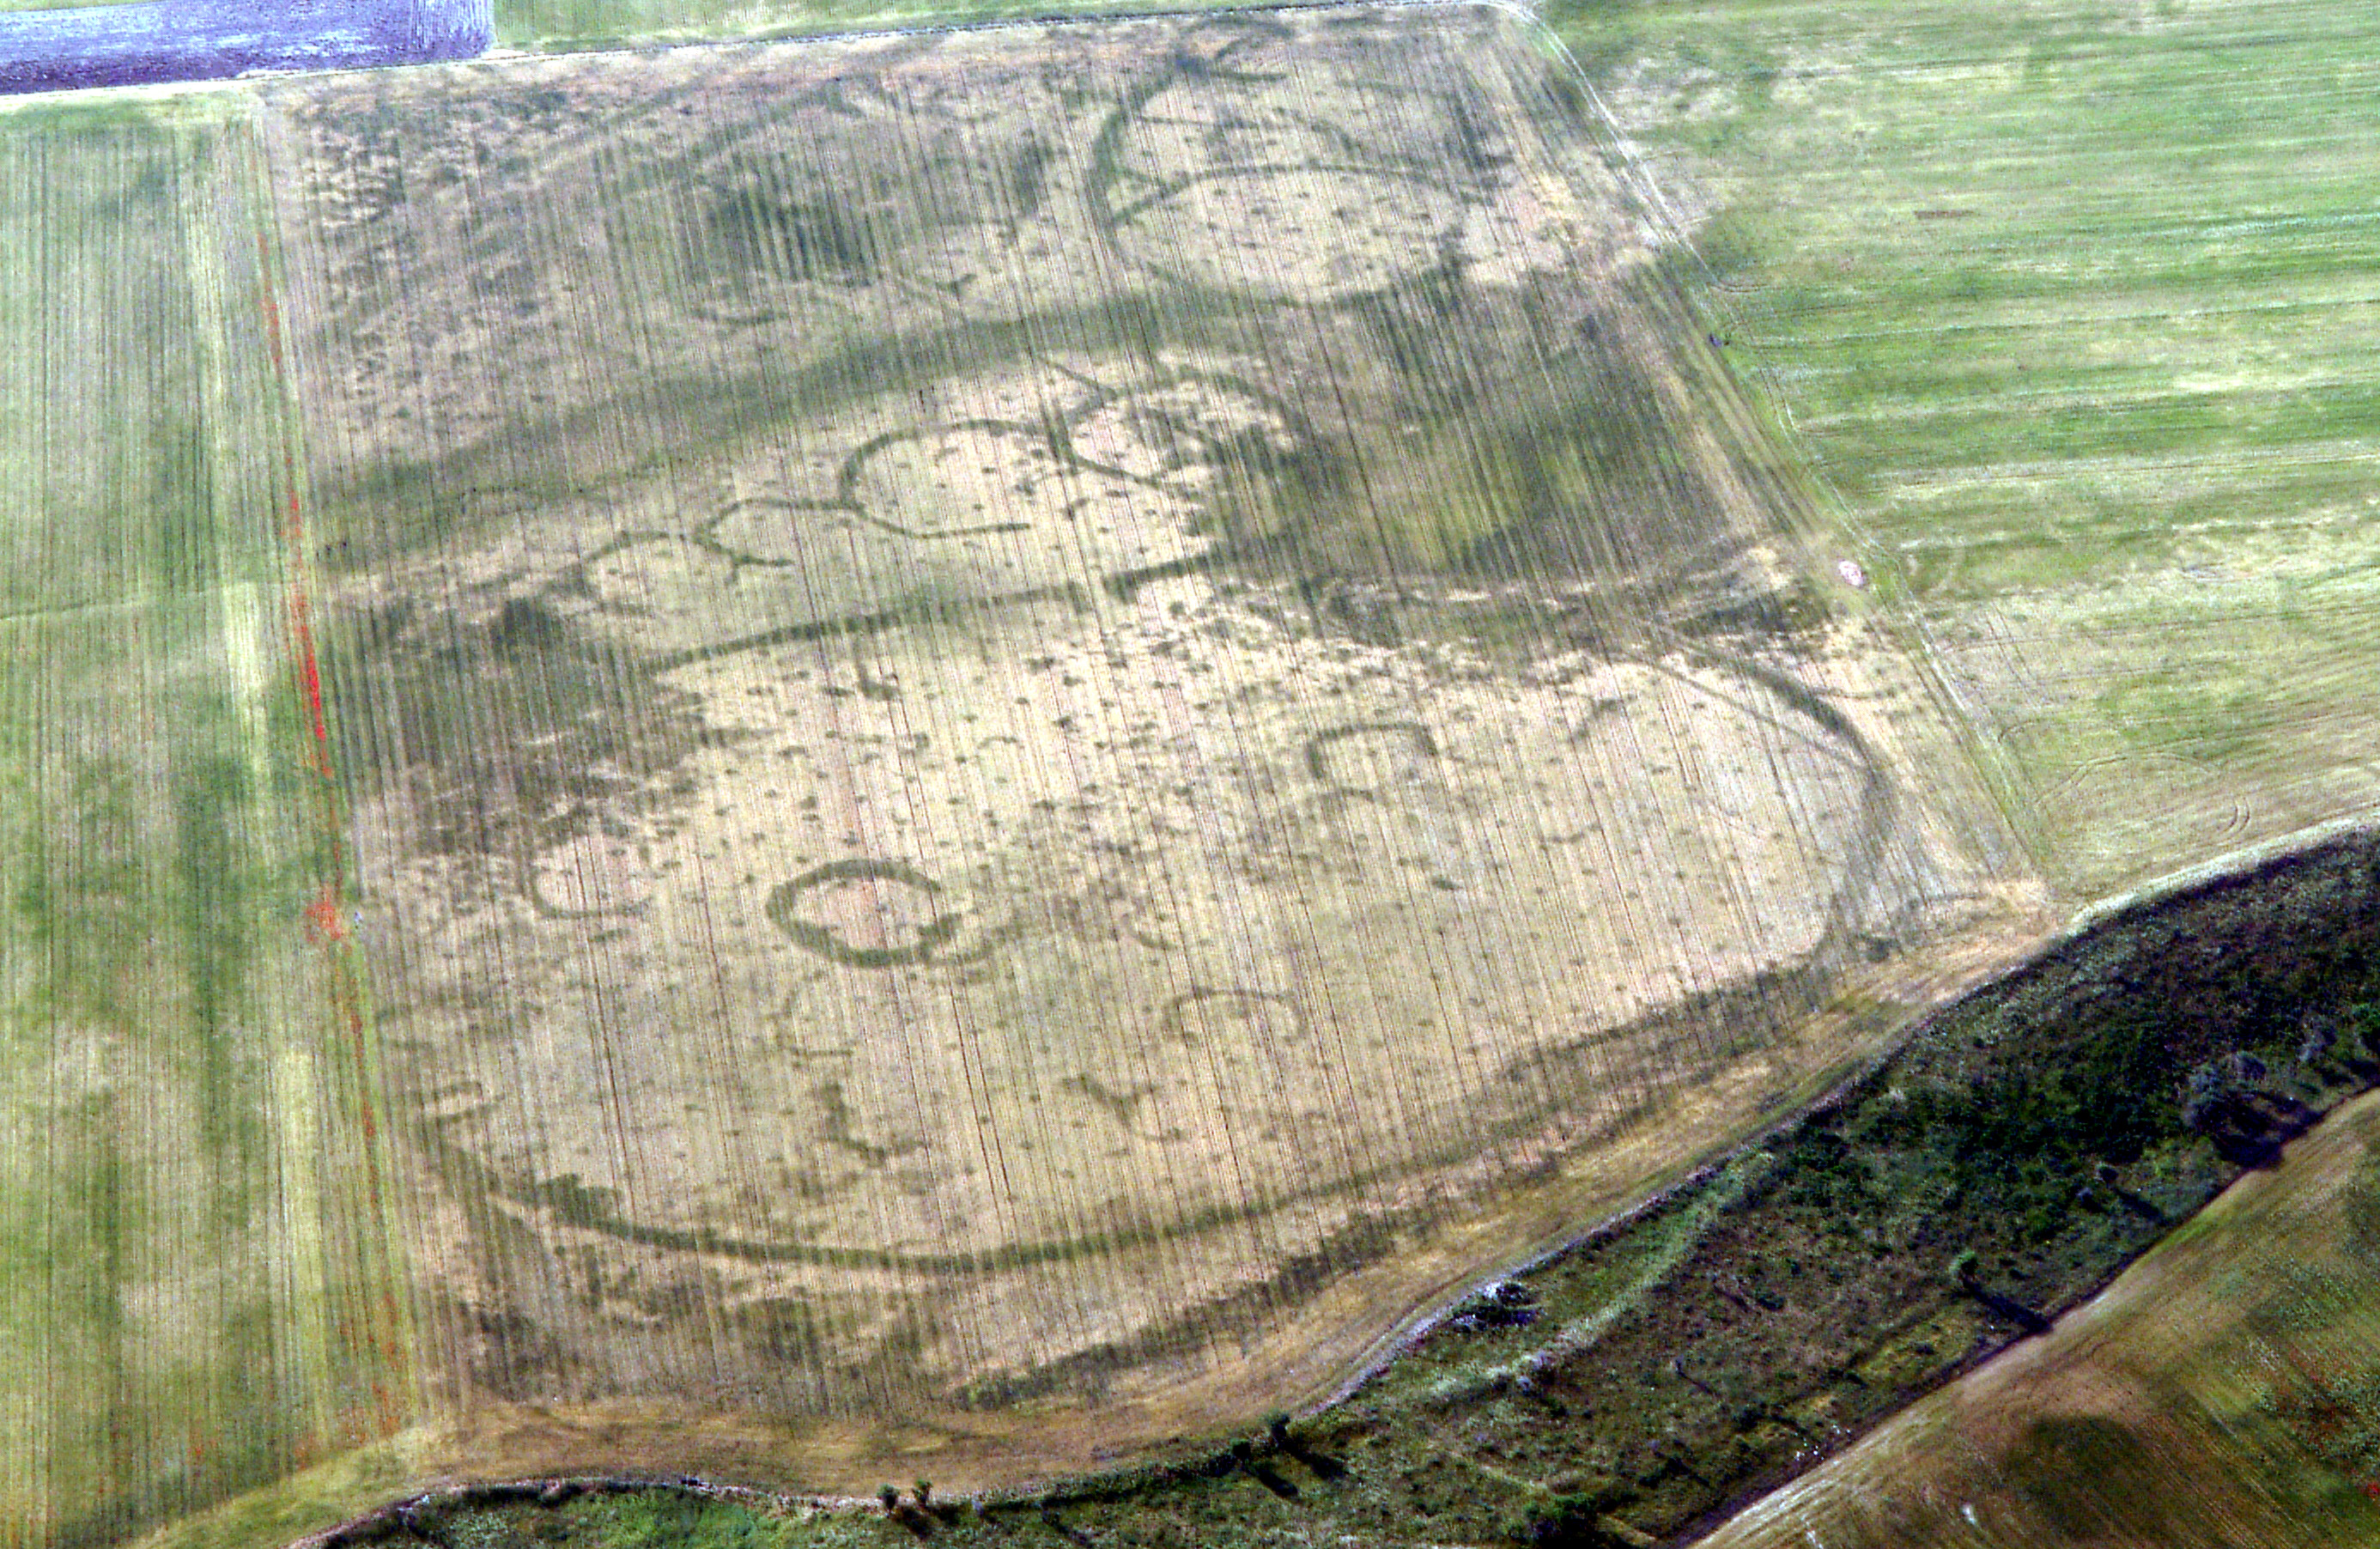
\includegraphics[width=\textwidth]{img/aerea}};
            \pause
            \draw [thick,draw=red,double] (7.1,4) -- (7.3,3.9) -- (7.5,3.84) -- (7.8,3.7) -- (8.1,3.5) -- (8.2,3.3) -- (7.9,2.5) -- (6.7,1.85) -- (5.5,1.5) -- (5,1.35) -- (4.5,1.3) -- (3.8,1.25) -- (3.4,1.3) -- (3,1.35) -- (2.8,1.38) -- (2.7,1.4) -- (2.4,1.5) -- (2,1.65) -- (1.8,1.8);
            \draw [thick,draw=red,double] (2.8,3.8) -- (3.2,3.9) -- (4.68,4.15) -- (4.7,4.05);
            \draw [thick,draw=red,double] (4.89,4.05) -- (4.85,4.18) -- (6,4.3);
            \node [thick,draw=blue!50,fill=black!10,rounded corners] (ditch-label) at (6.8,4.6) {\tiny{ditch}};
            \pause
            \node [draw,thick,dashed,circle,inner sep=9pt] (comp1) at (3.75,2.8) {};
            \node [draw,thick,dashed,circle,inner sep=9pt] (comp2) at (5.35,2.3) {};
            \node [draw,thick,dashed,circle,inner sep=9pt] (comp3) at (5.95,3.45) {};
            \node [thick,draw=blue!50,fill=black!10,rounded corners] (compound-label) at (6.7,2.6) {\tiny{compounds}};
            \draw [->] (compound-label.west) to [bend right=30] (comp1);
            \draw [->] (compound-label.south) to [bend left=30] (comp2);
            \draw [->] (compound-label.north) to [bend right=20] (comp3);
        \end{tikzpicture}
    \end{frame}

    \section{Workflow}
        \begin{frame}{Il workflow dell'analisi geofisica}
            \resizebox{1\textwidth}{!}{%
                \begin{tikzpicture}
                    \input{img/dot-flow-general}
                \end{tikzpicture}
            }
        \end{frame}

        \begin{frame}{Il workflow dell'analisi geofisica}
            \resizebox{1\textwidth}{!}{%
                \begin{tikzpicture}
                    \input{img/dot-flow-general-1}
                \end{tikzpicture}
            }
        \end{frame}

        \begin{frame}{Il workflow dell'analisi geofisica}
            \resizebox{1\textwidth}{!}{%
                \begin{tikzpicture}
                    \input{img/dot-flow-general-2}
                \end{tikzpicture}
            }
        \end{frame}

    \section{Compounds}
        \begin{frame}{Compounds: difficoltà e stato dell'arte}
            \begin{columns}[c]
                \column{0.5\textwidth}
                \centering
                \only<1>{
                    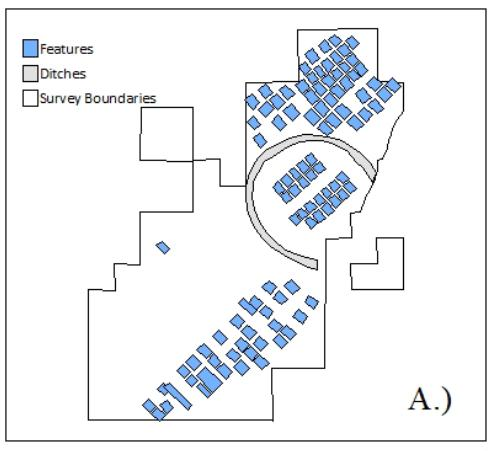
\includegraphics[width=0.8\textwidth]{img/niekamp}\\
                    A. Niekamp --- 2013\\
                    Pietrele, Romania
                }
                \column{0.5\textwidth}
            \end{columns}
        \end{frame}

        \begin{frame}{Compounds: difficoltà e stato dell'arte}
            \begin{columns}[c]
                \column{0.5\textwidth}
                    \centering
                    \begin{tikzpicture}
                        %\draw [help lines] (0,0) grid (4,3);
                        \draw [very thick,draw=blue!50,fill=black!20,rounded corners] (0,0) rectangle (1.5,2);
                        \draw[red,->] (0.75,-0.2) -- (0.75,2.5);
                    \end{tikzpicture}\\
                    A. Niekamp --- 2013\\
                    Pietrele, Romania
                \pause
                \column{0.5\textwidth}
                    \centering
                    \only<2-3>{
                        \begin{tikzpicture}[scale=0.007]
                            % simplified path created using Inkscape: path -> simplify
\begin{scope}[shift={(-1.80372,0)},draw=black,fill=blue!30,line join=round,line width=0.208pt]
    \path[draw,fill] (217.0000,188.0000) .. controls (196.1130,188.5005) and
      (198.7069,156.7044) .. (217.5032,155.4949) .. controls (256.9513,127.3325) and
      (305.7653,111.9178) .. (354.2431,112.8830) .. controls (404.0963,114.7639) and
      (455.7899,138.4646) .. (480.7256,183.3223) .. controls (499.6505,217.4627) and
      (497.9265,259.8457) .. (482.5888,294.9723) .. controls (472.9600,324.6744) and
      (464.2261,357.1967) .. (439.0720,377.9365) .. controls (417.9994,398.7900) and
      (389.2643,416.0558) .. (358.4901,411.4156) .. controls (333.3526,410.0387) and
      (309.1091,402.6746) .. (285.6851,393.9739) .. controls (256.2231,386.0058) and
      (222.7512,375.5693) .. (207.5772,346.5405) .. controls (196.0559,333.4033) and
      (202.3874,303.1015) .. (223.4951,317.0967) .. controls (239.6670,327.0899) and
      (241.3149,349.0555) .. (257.5391,359.4183) .. controls (278.3211,376.9693) and
      (305.5468,383.0352) .. (331.7729,386.8020) .. controls (345.3492,391.1707) and
      (358.8642,398.1856) .. (373.6579,396.0391) .. controls (393.9402,394.5193) and
      (409.3260,378.2529) .. (417.0111,360.4774) .. controls (423.8197,346.6240) and
      (435.6868,336.0929) .. (441.1463,321.4181) .. controls (453.9871,295.3612) and
      (456.7644,265.4984) .. (451.7422,237.1025) .. controls (449.8831,219.7295) and
      (451.9930,201.2927) .. (442.6174,185.5821) .. controls (424.8486,150.8474) and
      (384.8539,134.6999) .. (347.7452,131.9279) .. controls (317.7922,129.7260) and
      (287.1739,137.8572) .. (263.1078,156.0896) .. controls (247.8301,166.8719) and
      (232.7156,177.8551) .. (217.0000,188.0000) -- cycle;
\end{scope}

                            \begin{scope}[yshift=210em,xshift=150em,scale=0.90]
                                % simplified path created using Inkscape: path -> simplify
\begin{scope}[draw=black,fill=black!20,line join=round,line width=0.208pt]
    \path[draw,fill] (178.0000,123.0000) .. controls (206.3899,105.1174) and
      (231.9963,82.4401) .. (262.8309,68.6966) .. controls (281.3269,63.1992) and
      (300.9394,62.9002) .. (320.0559,62.7052) .. controls (359.4322,66.5280) and
      (398.8080,89.1213) .. (415.9989,125.6689) .. controls (422.5574,143.9788) and
      (419.7668,163.9287) .. (424.6156,182.6204) .. controls (428.4230,210.1111) and
      (422.8775,238.3834) .. (410.2254,262.9365) .. controls (403.2668,279.8945) and
      (388.6122,292.4669) .. (382.9050,310.0847) .. controls (368.7318,335.4133) and
      (332.3289,345.0550) .. (307.5175,329.8247) .. controls (290.5964,323.3461) and
      (271.7841,324.3546) .. (255.0611,317.0803) .. controls (237.7024,311.3261) and
      (222.8244,299.8380) .. (209.5819,287.7339) .. controls (201.6422,274.5835) and
      (195.9393,254.4474) .. (177.2237,254.4901) .. controls (163.7504,256.0115) and
      (163.5038,243.9714) .. (165.8854,234.6276) .. controls (169.9236,197.4184) and
      (173.9618,160.2092) .. (178.0000,123.0000) -- cycle;
\end{scope}

                            \end{scope}
                        \end{tikzpicture}
                        \pause
                        \begin{tikzpicture}[remember picture,overlay]
                            \node (per) at (0.5,1) {\tiny perimetro};
                            \node (area) at (-1.7,-0.5) {\tiny area};
                            \node[align=center] (acc-up) at (-3,2.5) {\tiny orientazione};
                            \node[align=center] (acc) at (-3,2.2) {\tiny (accesso)};
                            \draw[draw=red,fill=red] (-2.15,1.38) circle (1pt) coordinate(acc-n);
                            \draw[draw=red,fill=red] (-2.08,0.6) circle (1pt) coordinate(acc-s);
                            \draw[draw=red,fill=red] (acc-n) -- (acc-s);
                            \draw[->,>=*] (acc.south) to [bend right=55] ($ (acc-n)!.5!(acc-s) $);
                            \draw[->,>=*] (area.north) to [bend right=10] (-1.2,1);
                            \draw[->,>=*] (per.south) to [bend left=65] (-0.8,0.5);
                        \end{tikzpicture}
                    }
                    \pause
                    \begin{tikzpicture}[overlay,scale=0.007,yshift=-224cm,xshift=-368cm]
                        % simplified path created using Inkscape: path -> simplify
\begin{scope}[shift={(-1.80372,0)},draw=black,fill=blue!30,line join=round,line width=0.208pt]
    \path[draw,fill] (217.0000,188.0000) .. controls (196.1130,188.5005) and
      (198.7069,156.7044) .. (217.5032,155.4949) .. controls (256.9513,127.3325) and
      (305.7653,111.9178) .. (354.2431,112.8830) .. controls (404.0963,114.7639) and
      (455.7899,138.4646) .. (480.7256,183.3223) .. controls (499.6505,217.4627) and
      (497.9265,259.8457) .. (482.5888,294.9723) .. controls (472.9600,324.6744) and
      (464.2261,357.1967) .. (439.0720,377.9365) .. controls (417.9994,398.7900) and
      (389.2643,416.0558) .. (358.4901,411.4156) .. controls (333.3526,410.0387) and
      (309.1091,402.6746) .. (285.6851,393.9739) .. controls (256.2231,386.0058) and
      (222.7512,375.5693) .. (207.5772,346.5405) .. controls (196.0559,333.4033) and
      (202.3874,303.1015) .. (223.4951,317.0967) .. controls (239.6670,327.0899) and
      (241.3149,349.0555) .. (257.5391,359.4183) .. controls (278.3211,376.9693) and
      (305.5468,383.0352) .. (331.7729,386.8020) .. controls (345.3492,391.1707) and
      (358.8642,398.1856) .. (373.6579,396.0391) .. controls (393.9402,394.5193) and
      (409.3260,378.2529) .. (417.0111,360.4774) .. controls (423.8197,346.6240) and
      (435.6868,336.0929) .. (441.1463,321.4181) .. controls (453.9871,295.3612) and
      (456.7644,265.4984) .. (451.7422,237.1025) .. controls (449.8831,219.7295) and
      (451.9930,201.2927) .. (442.6174,185.5821) .. controls (424.8486,150.8474) and
      (384.8539,134.6999) .. (347.7452,131.9279) .. controls (317.7922,129.7260) and
      (287.1739,137.8572) .. (263.1078,156.0896) .. controls (247.8301,166.8719) and
      (232.7156,177.8551) .. (217.0000,188.0000) -- cycle;
\end{scope}

                    \end{tikzpicture}
                    \begin{tikzpicture}[remember picture,overlay]
                        \node (label) at (-0.5,-1.22) {A. Laterza --- 2013};
                        \node (label) at (-0.5,-1.7) {Tavoliere, Puglia};
                    \end{tikzpicture}
            \end{columns}
        \end{frame}

    \section{Distinzione}
        \begin{frame}{Distinzione di \emph{ditches} e \emph{compounds}: Jenks}
            \small{Anglisano (Lucera): 47 geometrie}\\
            \centering
            \scalebox{1}[-1]{ % mirror image
                \begin{tikzpicture}[x=1mm,y=1mm,scale=0.15]
                    \definecolor{cff0000}{RGB}{255,255,255}
\definecolor{c2b83ba}{RGB}{255,255,255}
\definecolor{cabdda4}{RGB}{255,255,255}
\definecolor{cffffbf}{RGB}{255,255,255}
\definecolor{cfdae61}{RGB}{255,255,255}
\definecolor{cd7191c}{RGB}{255,255,255}

\begin{scope}[draw=black,fill=cd7191c,line join=round,line width=0.208pt]
  \path[draw,fill] (545.0000,190.0000) -- (544.0000,191.0000) --
    (543.0000,191.0000) -- (543.0000,190.0000) -- (543.0000,189.0000) --
    (544.0000,188.0000) -- (545.0000,187.0000) -- (546.0000,187.0000) --
    (548.0000,181.0000) -- (548.0000,180.0000) -- (548.0000,179.0000) --
    (548.0000,178.0000) -- (547.0000,177.0000) -- (547.0000,176.0000) --
    (546.0000,176.0000) -- (547.0000,176.0000) -- (547.0000,175.0000) --
    (548.0000,175.0000) -- (549.0000,176.0000) -- (550.0000,178.0000) --
    (550.0000,180.0000) -- (550.0000,182.0000) -- (549.0000,184.0000) --
    (548.0000,185.0000) -- (545.0000,190.0000);
  \path[draw,fill] (538.0000,191.0000) -- (537.0000,191.0000) --
    (536.0000,191.0000) -- (535.0000,191.0000) -- (534.0000,191.0000) --
    (533.0000,190.0000) -- (531.0000,190.0000) -- (531.0000,189.0000) --
    (529.0000,185.0000) -- (528.0000,182.0000) -- (528.0000,181.0000) --
    (528.0000,179.0000) -- (529.0000,178.0000) -- (530.0000,176.0000) --
    (531.0000,175.0000) -- (532.0000,173.0000) -- (532.0000,172.0000) --
    (533.0000,172.0000) -- (533.0000,171.0000) -- (534.0000,171.0000) --
    (535.0000,171.0000) -- (536.0000,171.0000) -- (535.0000,172.0000) --
    (533.0000,175.0000) -- (532.0000,175.0000) -- (531.0000,177.0000) --
    (530.0000,178.0000) -- (530.0000,180.0000) -- (530.0000,182.0000) --
    (530.0000,183.0000) -- (530.0000,184.0000) -- (531.0000,185.0000) --
    (532.0000,187.0000) -- (533.0000,188.0000) -- (534.0000,189.0000) --
    (535.0000,190.0000) -- (538.0000,191.0000);
  \path[draw,fill] (339.0000,356.0000) -- (338.0000,356.0000) --
    (338.0000,355.0000) -- (338.0000,354.0000) -- (339.0000,353.0000) --
    (339.0000,352.0000) -- (340.0000,351.0000) -- (341.0000,351.0000) --
    (342.0000,350.0000) -- (343.0000,350.0000) -- (344.0000,350.0000) --
    (345.0000,350.0000) -- (346.0000,350.0000) -- (347.0000,351.0000) --
    (349.0000,351.0000) -- (351.0000,352.0000) -- (352.0000,353.0000) --
    (353.0000,354.0000) -- (354.0000,355.0000) -- (355.0000,357.0000) --
    (355.0000,359.0000) -- (355.0000,360.0000) -- (355.0000,362.0000) --
    (355.0000,364.0000) -- (354.0000,365.0000) -- (354.0000,366.0000) --
    (353.0000,366.0000) -- (353.0000,367.0000) -- (352.0000,368.0000) --
    (352.0000,369.0000) -- (351.0000,369.0000) -- (350.0000,370.0000) --
    (349.0000,370.0000) -- (348.0000,370.0000) -- (347.0000,370.0000) --
    (347.0000,369.0000) -- (346.0000,369.0000) -- (345.0000,369.0000) --
    (344.0000,369.0000) -- (343.0000,368.0000) -- (342.0000,368.0000) --
    (341.0000,367.0000) -- (340.0000,365.0000) -- (339.0000,364.0000) --
    (343.0000,364.0000) -- (347.0000,364.0000) -- (347.0000,363.0000) --
    (348.0000,363.0000) -- (349.0000,362.0000) -- (349.0000,361.0000) --
    (349.0000,360.0000) -- (349.0000,359.0000) -- (349.0000,358.0000) --
    (349.0000,357.0000) -- (348.0000,357.0000) -- (348.0000,356.0000) --
    (347.0000,356.0000) -- (346.0000,355.0000) -- (345.0000,355.0000) --
    (344.0000,354.0000) -- (343.0000,354.0000) -- (342.0000,353.0000) --
    (341.0000,354.0000) -- (340.0000,354.0000) -- (340.0000,355.0000) --
    (339.0000,355.0000) -- (339.0000,356.0000);
  \path[draw,fill] (330.0000,344.0000) -- (342.0000,343.0000) --
    (343.0000,342.0000) -- (343.0000,341.0000) -- (344.0000,340.0000) --
    (344.0000,339.0000) -- (344.0000,337.0000) -- (344.0000,336.0000) --
    (344.0000,335.0000) -- (344.0000,334.0000) -- (343.0000,333.0000) --
    (342.0000,332.0000) -- (341.0000,331.0000) -- (340.0000,331.0000) --
    (334.0000,331.0000) -- (336.0000,326.0000) -- (341.0000,328.0000) --
    (347.0000,330.0000) -- (348.0000,331.0000) -- (349.0000,333.0000) --
    (349.0000,335.0000) -- (349.0000,336.0000) -- (349.0000,338.0000) --
    (349.0000,340.0000) -- (348.0000,342.0000) -- (347.0000,343.0000) --
    (345.0000,345.0000) -- (333.0000,347.0000) -- (330.0000,344.0000);
  \path[draw,fill] (424.0000,299.0000) -- (421.0000,292.0000) --
    (425.0000,289.0000) -- (429.0000,286.0000) -- (431.0000,286.0000) --
    (432.0000,285.0000) -- (437.0000,286.0000) -- (441.0000,287.0000) --
    (442.0000,288.0000) -- (445.0000,289.0000) -- (446.0000,290.0000) --
    (447.0000,291.0000) -- (448.0000,292.0000) -- (449.0000,294.0000) --
    (449.0000,295.0000) -- (449.0000,297.0000) -- (449.0000,298.0000) --
    (450.0000,299.0000) -- (450.0000,300.0000) -- (450.0000,301.0000) --
    (449.0000,302.0000) -- (448.0000,302.0000) -- (447.0000,302.0000) --
    (446.0000,302.0000) -- (446.0000,301.0000) -- (446.0000,300.0000) --
    (447.0000,295.0000) -- (447.0000,293.0000) -- (444.0000,291.0000) --
    (438.0000,288.0000) -- (436.0000,288.0000) -- (434.0000,288.0000) --
    (432.0000,288.0000) -- (430.0000,289.0000) -- (429.0000,290.0000) --
    (427.0000,291.0000) -- (427.0000,292.0000) -- (425.0000,295.0000) --
    (424.0000,298.0000) -- (424.0000,299.0000);
  \path[draw,fill] (380.0000,263.0000) -- (380.0000,261.0000) --
    (381.0000,260.0000) -- (383.0000,259.0000) -- (385.0000,259.0000) --
    (387.0000,259.0000) -- (389.0000,259.0000) -- (391.0000,259.0000) --
    (392.0000,260.0000) -- (393.0000,261.0000) -- (394.0000,262.0000) --
    (395.0000,262.0000) -- (396.0000,266.0000) -- (396.0000,271.0000) --
    (395.0000,276.0000) -- (395.0000,279.0000) -- (394.0000,280.0000) --
    (393.0000,282.0000) -- (391.0000,284.0000) -- (389.0000,285.0000) --
    (387.0000,286.0000) -- (384.0000,287.0000) -- (384.0000,288.0000) --
    (383.0000,288.0000) -- (383.0000,289.0000) -- (382.0000,289.0000) --
    (381.0000,289.0000) -- (380.0000,289.0000) -- (380.0000,288.0000) --
    (379.0000,288.0000) -- (379.0000,287.0000) -- (382.0000,285.0000) --
    (387.0000,283.0000) -- (392.0000,279.0000) -- (392.0000,278.0000) --
    (393.0000,274.0000) -- (394.0000,270.0000) -- (393.0000,266.0000) --
    (392.0000,262.0000) -- (389.0000,261.0000) -- (385.0000,261.0000) --
    (382.0000,262.0000) -- (380.0000,263.0000);
  \path[draw,fill] (334.0000,431.0000) -- (333.0000,431.0000) --
    (333.0000,430.0000) -- (333.0000,429.0000) -- (334.0000,429.0000) --
    (334.0000,428.0000) -- (335.0000,428.0000) -- (336.0000,428.0000) --
    (336.0000,429.0000) -- (337.0000,429.0000) -- (338.0000,429.0000) --
    (339.0000,429.0000) -- (340.0000,429.0000) -- (341.0000,430.0000) --
    (342.0000,431.0000) -- (342.0000,432.0000) -- (343.0000,433.0000) --
    (342.0000,434.0000) -- (343.0000,434.0000) -- (343.0000,437.0000) --
    (342.0000,440.0000) -- (341.0000,443.0000) -- (339.0000,444.0000) --
    (337.0000,444.0000) -- (336.0000,444.0000) -- (334.0000,443.0000) --
    (333.0000,443.0000) -- (333.0000,442.0000) -- (333.0000,441.0000) --
    (333.0000,440.0000) -- (334.0000,439.0000) -- (334.0000,438.0000) --
    (335.0000,438.0000) -- (336.0000,439.0000) -- (337.0000,439.0000) --
    (338.0000,439.0000) -- (339.0000,438.0000) -- (340.0000,438.0000) --
    (340.0000,437.0000) -- (341.0000,437.0000) -- (341.0000,436.0000) --
    (341.0000,435.0000) -- (340.0000,434.0000) -- (340.0000,433.0000) --
    (339.0000,432.0000) -- (338.0000,432.0000) -- (334.0000,431.0000);
  \path[draw,fill] (438.0000,204.0000) -- (435.0000,202.0000) --
    (438.0000,198.0000) -- (442.0000,196.0000) -- (445.0000,196.0000) --
    (447.0000,195.0000) -- (448.0000,195.0000) -- (451.0000,199.0000) --
    (453.0000,202.0000) -- (454.0000,204.0000) -- (454.0000,205.0000) --
    (454.0000,206.0000) -- (454.0000,207.0000) -- (454.0000,208.0000) --
    (453.0000,209.0000) -- (451.0000,209.0000) -- (449.0000,208.0000) --
    (450.0000,206.0000) -- (451.0000,203.0000) -- (450.0000,202.0000) --
    (450.0000,201.0000) -- (449.0000,200.0000) -- (448.0000,199.0000) --
    (446.0000,199.0000) -- (445.0000,198.0000) -- (438.0000,204.0000);
  \path[draw,fill] (486.0000,193.0000) -- (486.0000,192.0000) --
    (487.0000,192.0000) -- (490.0000,195.0000) -- (496.0000,200.0000) --
    (501.0000,207.0000) -- (502.0000,210.0000) -- (502.0000,211.0000) --
    (503.0000,212.0000) -- (503.0000,214.0000) -- (503.0000,215.0000) --
    (502.0000,217.0000) -- (502.0000,218.0000) -- (501.0000,219.0000) --
    (500.0000,220.0000) -- (499.0000,220.0000) -- (499.0000,221.0000) --
    (498.0000,221.0000) -- (497.0000,221.0000) -- (497.0000,220.0000) --
    (498.0000,220.0000) -- (499.0000,219.0000) -- (500.0000,217.0000) --
    (500.0000,215.0000) -- (501.0000,213.0000) -- (500.0000,211.0000) --
    (500.0000,209.0000) -- (499.0000,207.0000) -- (498.0000,206.0000) --
    (498.0000,205.0000) -- (488.0000,196.0000) -- (486.0000,193.0000);
  \path[draw,fill] (470.0000,200.0000) -- (471.0000,197.0000) --
    (475.0000,194.0000) -- (478.0000,192.0000) -- (478.0000,193.0000) --
    (475.0000,195.0000) -- (472.0000,198.0000) -- (471.0000,200.0000) --
    (470.0000,200.0000);
  \path[draw,fill] (624.0000,323.0000) -- (626.0000,322.0000) --
    (629.0000,320.0000) -- (630.0000,319.0000) -- (630.0000,318.0000) --
    (630.0000,317.0000) -- (630.0000,316.0000) -- (630.0000,315.0000) --
    (630.0000,314.0000) -- (629.0000,314.0000) -- (628.0000,313.0000) --
    (627.0000,313.0000) -- (626.0000,313.0000) -- (625.0000,313.0000) --
    (625.0000,314.0000) -- (624.0000,314.0000) -- (623.0000,314.0000) --
    (622.0000,313.0000) -- (622.0000,312.0000) -- (623.0000,311.0000) --
    (624.0000,311.0000) -- (626.0000,311.0000) -- (627.0000,311.0000) --
    (628.0000,312.0000) -- (630.0000,312.0000) -- (630.0000,313.0000) --
    (631.0000,313.0000) -- (631.0000,314.0000) -- (631.0000,315.0000) --
    (632.0000,316.0000) -- (632.0000,317.0000) -- (631.0000,318.0000) --
    (631.0000,319.0000) -- (631.0000,320.0000) -- (631.0000,321.0000) --
    (630.0000,321.0000) -- (630.0000,322.0000) -- (629.0000,322.0000) --
    (628.0000,323.0000) -- (627.0000,323.0000) -- (627.0000,324.0000) --
    (626.0000,324.0000) -- (625.0000,324.0000) -- (624.0000,323.0000);
\end{scope}
\begin{scope}[draw=black,fill=cfdae61,line join=round,line width=0.208pt]
  \path[draw,fill] (579.0000,127.0000) -- (580.0000,126.0000) --
    (583.0000,124.0000) -- (584.0000,123.0000) -- (585.0000,123.0000) --
    (587.0000,122.0000) -- (588.0000,122.0000) -- (590.0000,122.0000) --
    (592.0000,123.0000) -- (593.0000,124.0000) -- (594.0000,124.0000) --
    (596.0000,125.0000) -- (597.0000,127.0000) -- (598.0000,128.0000) --
    (599.0000,130.0000) -- (599.0000,131.0000) -- (598.0000,131.0000) --
    (598.0000,132.0000) -- (599.0000,133.0000) -- (599.0000,134.0000) --
    (598.0000,134.0000) -- (596.0000,138.0000) -- (593.0000,142.0000) --
    (590.0000,143.0000) -- (588.0000,143.0000) -- (587.0000,143.0000) --
    (586.0000,143.0000) -- (584.0000,143.0000) -- (583.0000,142.0000) --
    (581.0000,141.0000) -- (580.0000,140.0000) -- (579.0000,139.0000) --
    (577.0000,137.0000) -- (576.0000,135.0000) -- (575.0000,135.0000) --
    (575.0000,134.0000) -- (575.0000,133.0000) -- (575.0000,132.0000) --
    (575.0000,131.0000) -- (579.0000,127.0000);
  \path[draw,fill] (578.0000,136.0000) -- (589.0000,142.0000) --
    (593.0000,138.0000) -- (594.0000,137.0000) -- (595.0000,136.0000) --
    (595.0000,135.0000) -- (595.0000,134.0000) -- (596.0000,133.0000) --
    (596.0000,132.0000) -- (597.0000,131.0000) -- (597.0000,130.0000) --
    (596.0000,129.0000) -- (593.0000,127.0000) -- (590.0000,125.0000) --
    (587.0000,124.0000) -- (586.0000,124.0000) -- (586.0000,125.0000) --
    (585.0000,125.0000) -- (583.0000,127.0000) -- (580.0000,129.0000) --
    (578.0000,131.0000) -- (577.0000,132.0000) -- (577.0000,133.0000) --
    (576.0000,133.0000) -- (576.0000,134.0000) -- (577.0000,134.0000) --
    (577.0000,135.0000) -- (578.0000,135.0000) -- (578.0000,136.0000);
  \path[draw,fill] (608.0000,188.0000) -- (607.0000,188.0000) --
    (606.0000,189.0000) -- (605.0000,189.0000) -- (604.0000,190.0000) --
    (603.0000,192.0000) -- (602.0000,193.0000) -- (602.0000,194.0000) --
    (602.0000,196.0000) -- (602.0000,197.0000) -- (602.0000,198.0000) --
    (601.0000,199.0000) -- (601.0000,201.0000) -- (601.0000,202.0000) --
    (601.0000,203.0000) -- (601.0000,205.0000) -- (602.0000,206.0000) --
    (603.0000,207.0000) -- (604.0000,208.0000) -- (605.0000,209.0000) --
    (606.0000,210.0000) -- (607.0000,210.0000) -- (608.0000,210.0000) --
    (609.0000,210.0000) -- (614.0000,210.0000) -- (618.0000,211.0000) --
    (622.0000,213.0000) -- (623.0000,212.0000) -- (625.0000,212.0000) --
    (626.0000,211.0000) -- (627.0000,209.0000) -- (628.0000,208.0000) --
    (629.0000,206.0000) -- (630.0000,205.0000) -- (630.0000,204.0000) --
    (630.0000,205.0000) -- (631.0000,206.0000) -- (631.0000,207.0000) --
    (631.0000,208.0000) -- (631.0000,209.0000) -- (631.0000,210.0000) --
    (630.0000,210.0000) -- (630.0000,211.0000) -- (629.0000,212.0000) --
    (628.0000,212.0000) -- (627.0000,213.0000) -- (625.0000,214.0000) --
    (620.0000,214.0000) -- (614.0000,214.0000) -- (613.0000,214.0000) --
    (612.0000,214.0000) -- (608.0000,214.0000) -- (604.0000,213.0000) --
    (600.0000,211.0000) -- (600.0000,210.0000) -- (599.0000,210.0000) --
    (599.0000,209.0000) -- (598.0000,209.0000) -- (598.0000,208.0000) --
    (598.0000,207.0000) -- (598.0000,206.0000) -- (598.0000,205.0000) --
    (598.0000,204.0000) -- (599.0000,203.0000) -- (599.0000,202.0000) --
    (598.0000,201.0000) -- (598.0000,200.0000) -- (597.0000,199.0000) --
    (597.0000,198.0000) -- (597.0000,197.0000) -- (598.0000,196.0000) --
    (598.0000,195.0000) -- (598.0000,193.0000) -- (599.0000,191.0000) --
    (600.0000,190.0000) -- (602.0000,188.0000) -- (603.0000,187.0000) --
    (605.0000,186.0000) -- (608.0000,188.0000);
  \path[draw,fill] (534.0000,261.0000) -- (532.0000,261.0000) --
    (529.0000,263.0000) -- (526.0000,265.0000) -- (524.0000,269.0000) --
    (523.0000,270.0000) -- (521.0000,272.0000) -- (520.0000,275.0000) --
    (520.0000,276.0000) -- (524.0000,281.0000) -- (529.0000,286.0000) --
    (533.0000,290.0000) -- (538.0000,292.0000) -- (541.0000,293.0000) --
    (542.0000,293.0000) -- (544.0000,293.0000) -- (545.0000,293.0000) --
    (546.0000,293.0000) -- (547.0000,292.0000) -- (547.0000,291.0000) --
    (548.0000,290.0000) -- (548.0000,289.0000) -- (547.0000,289.0000) --
    (546.0000,288.0000) -- (546.0000,287.0000) -- (545.0000,286.0000) --
    (546.0000,285.0000) -- (547.0000,285.0000) -- (548.0000,285.0000) --
    (548.0000,286.0000) -- (549.0000,287.0000) -- (548.0000,287.0000) --
    (549.0000,288.0000) -- (550.0000,288.0000) -- (551.0000,288.0000) --
    (552.0000,288.0000) -- (552.0000,287.0000) -- (553.0000,287.0000) --
    (553.0000,283.0000) -- (553.0000,282.0000) -- (554.0000,282.0000) --
    (555.0000,282.0000) -- (555.0000,283.0000) -- (556.0000,283.0000) --
    (557.0000,284.0000) -- (557.0000,285.0000) -- (557.0000,286.0000) --
    (558.0000,286.0000) -- (557.0000,287.0000) -- (553.0000,289.0000) --
    (550.0000,292.0000) -- (548.0000,294.0000) -- (546.0000,295.0000) --
    (542.0000,295.0000) -- (538.0000,295.0000) -- (536.0000,294.0000) --
    (533.0000,293.0000) -- (528.0000,289.0000) -- (523.0000,284.0000) --
    (521.0000,283.0000) -- (519.0000,281.0000) -- (517.0000,279.0000) --
    (516.0000,276.0000) -- (516.0000,275.0000) -- (517.0000,274.0000) --
    (518.0000,272.0000) -- (519.0000,271.0000) -- (520.0000,270.0000) --
    (521.0000,269.0000) -- (522.0000,269.0000) -- (522.0000,267.0000) --
    (525.0000,264.0000) -- (528.0000,262.0000) -- (531.0000,260.0000) --
    (533.0000,259.0000) -- (534.0000,261.0000);
  \path[draw,fill] (512.0000,285.0000) -- (508.0000,288.0000) --
    (505.0000,290.0000) -- (504.0000,292.0000) -- (501.0000,295.0000) --
    (500.0000,298.0000) -- (500.0000,299.0000) -- (500.0000,300.0000) --
    (500.0000,302.0000) -- (501.0000,303.0000) -- (502.0000,304.0000) --
    (503.0000,305.0000) -- (504.0000,306.0000) -- (505.0000,306.0000) --
    (507.0000,308.0000) -- (511.0000,311.0000) -- (515.0000,313.0000) --
    (516.0000,313.0000) -- (521.0000,314.0000) -- (526.0000,314.0000) --
    (527.0000,313.0000) -- (532.0000,308.0000) -- (533.0000,307.0000) --
    (533.0000,305.0000) -- (533.0000,304.0000) -- (533.0000,303.0000) --
    (534.0000,303.0000) -- (536.0000,303.0000) -- (536.0000,305.0000) --
    (535.0000,309.0000) -- (533.0000,312.0000) -- (530.0000,314.0000) --
    (529.0000,315.0000) -- (527.0000,316.0000) -- (525.0000,317.0000) --
    (523.0000,317.0000) -- (522.0000,317.0000) -- (520.0000,317.0000) --
    (518.0000,317.0000) -- (516.0000,316.0000) -- (515.0000,316.0000) --
    (508.0000,312.0000) -- (504.0000,310.0000) -- (503.0000,309.0000) --
    (500.0000,307.0000) -- (497.0000,303.0000) -- (496.0000,301.0000) --
    (496.0000,299.0000) -- (497.0000,296.0000) -- (499.0000,293.0000) --
    (500.0000,292.0000) -- (502.0000,289.0000) -- (505.0000,286.0000) --
    (508.0000,284.0000) -- (512.0000,285.0000);
  \path[draw,fill] (338.0000,398.0000) -- (338.0000,397.0000) --
    (337.0000,396.0000) -- (338.0000,395.0000) -- (338.0000,394.0000) --
    (339.0000,393.0000) -- (340.0000,394.0000) -- (341.0000,394.0000) --
    (343.0000,395.0000) -- (345.0000,395.0000) -- (347.0000,395.0000) --
    (349.0000,394.0000) -- (350.0000,394.0000) -- (351.0000,393.0000) --
    (352.0000,392.0000) -- (353.0000,391.0000) -- (353.0000,390.0000) --
    (354.0000,388.0000) -- (354.0000,387.0000) -- (354.0000,386.0000) --
    (353.0000,384.0000) -- (353.0000,383.0000) -- (348.0000,382.0000) --
    (343.0000,381.0000) -- (342.0000,381.0000) -- (338.0000,381.0000) --
    (338.0000,380.0000) -- (337.0000,380.0000) -- (337.0000,379.0000) --
    (338.0000,379.0000) -- (338.0000,378.0000) -- (338.0000,377.0000) --
    (339.0000,377.0000) -- (339.0000,376.0000) -- (340.0000,376.0000) --
    (341.0000,376.0000) -- (342.0000,376.0000) -- (343.0000,377.0000) --
    (344.0000,377.0000) -- (346.0000,376.0000) -- (349.0000,377.0000) --
    (351.0000,377.0000) -- (353.0000,378.0000) -- (355.0000,380.0000) --
    (356.0000,381.0000) -- (357.0000,382.0000) -- (358.0000,384.0000) --
    (359.0000,386.0000) -- (359.0000,388.0000) -- (359.0000,390.0000) --
    (358.0000,392.0000) -- (357.0000,394.0000) -- (357.0000,395.0000) --
    (357.0000,396.0000) -- (357.0000,397.0000) -- (356.0000,398.0000) --
    (356.0000,399.0000) -- (355.0000,400.0000) -- (354.0000,401.0000) --
    (353.0000,401.0000) -- (352.0000,401.0000) -- (351.0000,401.0000) --
    (350.0000,401.0000) -- (349.0000,401.0000) -- (348.0000,400.0000) --
    (338.0000,398.0000);
  \path[draw,fill] (348.0000,284.0000) -- (347.0000,285.0000) --
    (347.0000,286.0000) -- (346.0000,287.0000) -- (345.0000,288.0000) --
    (345.0000,289.0000) -- (345.0000,290.0000) -- (345.0000,292.0000) --
    (345.0000,293.0000) -- (346.0000,294.0000) -- (347.0000,295.0000) --
    (348.0000,296.0000) -- (350.0000,297.0000) -- (351.0000,297.0000) --
    (353.0000,297.0000) -- (354.0000,297.0000) -- (356.0000,297.0000) --
    (357.0000,296.0000) -- (358.0000,296.0000) -- (359.0000,296.0000) --
    (360.0000,296.0000) -- (360.0000,295.0000) -- (361.0000,295.0000) --
    (361.0000,294.0000) -- (362.0000,293.0000) -- (362.0000,292.0000) --
    (362.0000,291.0000) -- (362.0000,290.0000) -- (361.0000,289.0000) --
    (361.0000,288.0000) -- (361.0000,287.0000) -- (361.0000,286.0000) --
    (360.0000,285.0000) -- (360.0000,284.0000) -- (359.0000,283.0000) --
    (358.0000,282.0000) -- (357.0000,281.0000) -- (355.0000,281.0000) --
    (354.0000,281.0000) -- (354.0000,280.0000) -- (354.0000,279.0000) --
    (355.0000,279.0000) -- (355.0000,278.0000) -- (355.0000,279.0000) --
    (356.0000,279.0000) -- (356.0000,280.0000) -- (357.0000,280.0000) --
    (359.0000,281.0000) -- (360.0000,282.0000) -- (361.0000,283.0000) --
    (362.0000,284.0000) -- (363.0000,286.0000) -- (363.0000,288.0000) --
    (363.0000,289.0000) -- (363.0000,291.0000) -- (363.0000,292.0000) --
    (363.0000,293.0000) -- (363.0000,294.0000) -- (362.0000,296.0000) --
    (361.0000,297.0000) -- (361.0000,298.0000) -- (360.0000,298.0000) --
    (358.0000,299.0000) -- (357.0000,299.0000) -- (356.0000,299.0000) --
    (354.0000,300.0000) -- (352.0000,300.0000) -- (351.0000,300.0000) --
    (349.0000,299.0000) -- (347.0000,298.0000) -- (346.0000,298.0000) --
    (345.0000,297.0000) -- (343.0000,295.0000) -- (342.0000,294.0000) --
    (341.0000,292.0000) -- (341.0000,290.0000) -- (341.0000,288.0000) --
    (341.0000,287.0000) -- (341.0000,285.0000) -- (342.0000,284.0000) --
    (343.0000,283.0000) -- (344.0000,282.0000) -- (348.0000,284.0000);
  \path[draw,fill] (348.0000,307.0000) -- (348.0000,311.0000) --
    (348.0000,318.0000) -- (348.0000,319.0000) -- (348.0000,320.0000) --
    (348.0000,321.0000) -- (349.0000,321.0000) -- (349.0000,322.0000) --
    (350.0000,322.0000) -- (351.0000,323.0000) -- (352.0000,323.0000) --
    (353.0000,323.0000) -- (354.0000,323.0000) -- (355.0000,323.0000) --
    (356.0000,323.0000) -- (357.0000,323.0000) -- (358.0000,322.0000) --
    (359.0000,321.0000) -- (359.0000,320.0000) -- (359.0000,319.0000) --
    (359.0000,318.0000) -- (360.0000,318.0000) -- (360.0000,317.0000) --
    (361.0000,317.0000) -- (361.0000,316.0000) -- (362.0000,315.0000) --
    (362.0000,314.0000) -- (362.0000,313.0000) -- (362.0000,312.0000) --
    (361.0000,311.0000) -- (360.0000,310.0000) -- (359.0000,309.0000) --
    (357.0000,309.0000) -- (356.0000,308.0000) -- (356.0000,307.0000) --
    (357.0000,306.0000) -- (358.0000,305.0000) -- (359.0000,305.0000) --
    (359.0000,306.0000) -- (361.0000,307.0000) -- (363.0000,310.0000) --
    (365.0000,313.0000) -- (365.0000,314.0000) -- (365.0000,317.0000) --
    (363.0000,321.0000) -- (362.0000,323.0000) -- (361.0000,324.0000) --
    (359.0000,326.0000) -- (358.0000,327.0000) -- (356.0000,327.0000) --
    (354.0000,327.0000) -- (351.0000,326.0000) -- (349.0000,325.0000) --
    (347.0000,324.0000) -- (346.0000,323.0000) -- (346.0000,322.0000) --
    (345.0000,317.0000) -- (344.0000,313.0000) -- (344.0000,312.0000) --
    (344.0000,310.0000) -- (345.0000,309.0000) -- (346.0000,307.0000) --
    (346.0000,306.0000) -- (348.0000,307.0000);
  \path[draw,fill] (456.0000,248.0000) -- (462.0000,248.0000) --
    (467.0000,248.0000) -- (471.0000,246.0000) -- (473.0000,248.0000) --
    (467.0000,250.0000) -- (463.0000,252.0000) -- (459.0000,251.0000) --
    (454.0000,250.0000) -- (453.0000,250.0000) -- (451.0000,248.0000) --
    (448.0000,245.0000) -- (447.0000,242.0000) -- (446.0000,240.0000) --
    (446.0000,238.0000) -- (446.0000,236.0000) -- (446.0000,233.0000) --
    (446.0000,231.0000) -- (447.0000,229.0000) -- (449.0000,227.0000) --
    (451.0000,225.0000) -- (453.0000,224.0000) -- (453.0000,223.0000) --
    (455.0000,223.0000) -- (457.0000,222.0000) -- (460.0000,222.0000) --
    (462.0000,222.0000) -- (465.0000,223.0000) -- (467.0000,224.0000) --
    (469.0000,225.0000) -- (476.0000,228.0000) -- (475.0000,234.0000) --
    (474.0000,231.0000) -- (472.0000,229.0000) -- (469.0000,228.0000) --
    (467.0000,227.0000) -- (464.0000,226.0000) -- (462.0000,226.0000) --
    (459.0000,226.0000) -- (458.0000,226.0000) -- (456.0000,227.0000) --
    (455.0000,227.0000) -- (453.0000,228.0000) -- (452.0000,230.0000) --
    (451.0000,231.0000) -- (450.0000,233.0000) -- (450.0000,235.0000) --
    (449.0000,237.0000) -- (450.0000,238.0000) -- (450.0000,240.0000) --
    (451.0000,243.0000) -- (453.0000,246.0000) -- (456.0000,248.0000);
  \path[draw,fill] (295.0000,331.0000) -- (293.0000,333.0000) --
    (294.0000,332.0000) -- (295.0000,331.0000);
  \path[draw,fill] (293.0000,333.0000) -- (293.0000,334.0000) --
    (293.0000,335.0000) -- (293.0000,337.0000) -- (293.0000,338.0000) --
    (293.0000,339.0000) -- (294.0000,340.0000) -- (294.0000,341.0000) --
    (295.0000,342.0000) -- (296.0000,343.0000) -- (297.0000,344.0000) --
    (298.0000,345.0000) -- (299.0000,345.0000) -- (301.0000,346.0000) --
    (302.0000,346.0000) -- (304.0000,346.0000) -- (305.0000,345.0000) --
    (306.0000,345.0000) -- (307.0000,344.0000) -- (308.0000,344.0000) --
    (309.0000,343.0000) -- (310.0000,342.0000) -- (311.0000,341.0000) --
    (311.0000,340.0000) -- (312.0000,338.0000) -- (312.0000,337.0000) --
    (312.0000,336.0000) -- (311.0000,335.0000) -- (311.0000,334.0000) --
    (308.0000,332.0000) -- (304.0000,331.0000) -- (300.0000,330.0000) --
    (301.0000,330.0000) -- (303.0000,329.0000) -- (305.0000,328.0000) --
    (307.0000,328.0000) -- (309.0000,328.0000) -- (311.0000,329.0000) --
    (313.0000,330.0000) -- (314.0000,331.0000) -- (315.0000,334.0000) --
    (316.0000,336.0000) -- (316.0000,338.0000) -- (316.0000,340.0000) --
    (315.0000,342.0000) -- (314.0000,344.0000) -- (313.0000,346.0000) --
    (312.0000,347.0000) -- (311.0000,348.0000) -- (309.0000,349.0000) --
    (308.0000,350.0000) -- (306.0000,350.0000) -- (304.0000,351.0000) --
    (302.0000,350.0000) -- (300.0000,350.0000) -- (299.0000,349.0000) --
    (297.0000,348.0000) -- (296.0000,347.0000) -- (295.0000,345.0000) --
    (294.0000,345.0000) -- (293.0000,345.0000) -- (292.0000,344.0000) --
    (291.0000,343.0000) -- (290.0000,342.0000) -- (290.0000,341.0000) --
    (290.0000,340.0000) -- (290.0000,338.0000) -- (293.0000,333.0000);
  \path[draw,fill] (493.0000,193.0000) -- (492.0000,193.0000) --
    (493.0000,190.0000) -- (495.0000,187.0000) -- (497.0000,184.0000) --
    (498.0000,184.0000) -- (499.0000,183.0000) -- (500.0000,183.0000) --
    (501.0000,183.0000) -- (502.0000,183.0000) -- (503.0000,183.0000) --
    (504.0000,184.0000) -- (505.0000,184.0000) -- (506.0000,185.0000) --
    (507.0000,185.0000) -- (511.0000,188.0000) -- (515.0000,191.0000) --
    (519.0000,195.0000) -- (519.0000,196.0000) -- (520.0000,197.0000) --
    (520.0000,198.0000) -- (520.0000,199.0000) -- (520.0000,200.0000) --
    (520.0000,201.0000) -- (519.0000,202.0000) -- (518.0000,203.0000) --
    (517.0000,204.0000) -- (515.0000,205.0000) -- (510.0000,209.0000) --
    (508.0000,210.0000) -- (507.0000,210.0000) -- (507.0000,209.0000) --
    (509.0000,208.0000) -- (514.0000,204.0000) -- (518.0000,200.0000) --
    (518.0000,199.0000) -- (519.0000,198.0000) -- (518.0000,197.0000) --
    (518.0000,196.0000) -- (517.0000,195.0000) -- (513.0000,191.0000) --
    (506.0000,187.0000) -- (503.0000,185.0000) -- (502.0000,185.0000) --
    (501.0000,185.0000) -- (500.0000,185.0000) -- (499.0000,185.0000) --
    (498.0000,186.0000) -- (497.0000,186.0000) -- (497.0000,187.0000) --
    (496.0000,187.0000) -- (496.0000,188.0000) -- (496.0000,189.0000) --
    (493.0000,193.0000);
  \path[draw,fill] (402.0000,185.0000) -- (402.0000,182.0000) --
    (400.0000,181.0000) -- (401.0000,181.0000) -- (403.0000,179.0000) --
    (403.0000,178.0000) -- (404.0000,177.0000) -- (405.0000,177.0000) --
    (406.0000,176.0000) -- (407.0000,176.0000) -- (407.0000,175.0000) --
    (410.0000,173.0000) -- (413.0000,171.0000) -- (415.0000,170.0000) --
    (420.0000,170.0000) -- (423.0000,170.0000) -- (426.0000,171.0000) --
    (429.0000,174.0000) -- (430.0000,175.0000) -- (432.0000,177.0000) --
    (434.0000,179.0000) -- (434.0000,181.0000) -- (434.0000,182.0000) --
    (433.0000,182.0000) -- (432.0000,183.0000) -- (431.0000,183.0000) --
    (430.0000,184.0000) -- (428.0000,185.0000) -- (427.0000,186.0000) --
    (427.0000,188.0000) -- (426.0000,189.0000) -- (423.0000,192.0000) --
    (418.0000,197.0000) -- (416.0000,199.0000) -- (412.0000,196.0000) --
    (402.0000,185.0000);
  \path[draw,fill] (407.0000,178.0000) -- (406.0000,178.0000) --
    (405.0000,178.0000) -- (405.0000,179.0000) -- (404.0000,180.0000) --
    (404.0000,181.0000) -- (404.0000,182.0000) -- (403.0000,183.0000) --
    (404.0000,183.0000) -- (406.0000,187.0000) -- (409.0000,189.0000) --
    (412.0000,191.0000) -- (412.0000,192.0000) -- (413.0000,193.0000) --
    (414.0000,194.0000) -- (414.0000,195.0000) -- (415.0000,195.0000) --
    (416.0000,195.0000) -- (417.0000,195.0000) -- (422.0000,189.0000) --
    (423.0000,189.0000) -- (424.0000,188.0000) -- (425.0000,188.0000) --
    (425.0000,187.0000) -- (426.0000,186.0000) -- (426.0000,185.0000) --
    (428.0000,181.0000) -- (429.0000,180.0000) -- (429.0000,179.0000) --
    (429.0000,178.0000) -- (428.0000,177.0000) -- (428.0000,176.0000) --
    (427.0000,176.0000) -- (427.0000,175.0000) -- (426.0000,174.0000) --
    (425.0000,173.0000) -- (424.0000,172.0000) -- (422.0000,171.0000) --
    (421.0000,171.0000) -- (420.0000,171.0000) -- (418.0000,171.0000) --
    (416.0000,171.0000) -- (415.0000,172.0000) -- (414.0000,173.0000) --
    (413.0000,174.0000) -- (407.0000,178.0000);
\end{scope}
\begin{scope}[draw=black,fill=cffffbf,line join=round,line width=0.208pt]
  \path[draw,fill] (525.0000,442.0000) -- (515.0000,436.0000) --
    (512.0000,432.0000) -- (513.0000,432.0000) -- (515.0000,432.0000) --
    (516.0000,433.0000) -- (520.0000,436.0000) -- (521.0000,437.0000) --
    (522.0000,438.0000) -- (523.0000,438.0000) -- (524.0000,439.0000) --
    (525.0000,439.0000) -- (525.0000,442.0000);
  \path[draw,fill] (507.0000,423.0000) -- (506.0000,423.0000) --
    (505.0000,423.0000) -- (504.0000,423.0000) -- (503.0000,422.0000) --
    (503.0000,421.0000) -- (502.0000,421.0000) -- (502.0000,420.0000) --
    (502.0000,419.0000) -- (502.0000,418.0000) -- (501.0000,416.0000) --
    (498.0000,412.0000) -- (496.0000,407.0000) -- (495.0000,406.0000) --
    (494.0000,403.0000) -- (492.0000,399.0000) -- (492.0000,395.0000) --
    (492.0000,393.0000) -- (492.0000,391.0000) -- (491.0000,384.0000) --
    (490.0000,383.0000) -- (490.0000,382.0000) -- (490.0000,380.0000) --
    (490.0000,379.0000) -- (490.0000,378.0000) -- (491.0000,378.0000) --
    (492.0000,378.0000) -- (493.0000,379.0000) -- (493.0000,380.0000) --
    (494.0000,381.0000) -- (493.0000,381.0000) -- (494.0000,386.0000) --
    (495.0000,390.0000) -- (494.0000,395.0000) -- (497.0000,406.0000) --
    (500.0000,410.0000) -- (505.0000,417.0000) -- (507.0000,423.0000);
  \path[draw,fill] (486.0000,367.0000) -- (486.0000,363.0000) --
    (485.0000,359.0000) -- (485.0000,354.0000) -- (486.0000,349.0000) --
    (488.0000,345.0000) -- (489.0000,341.0000) -- (491.0000,337.0000) --
    (494.0000,334.0000) -- (496.0000,331.0000) -- (496.0000,330.0000) --
    (499.0000,327.0000) -- (502.0000,324.0000) -- (504.0000,323.0000) --
    (505.0000,322.0000) -- (506.0000,321.0000) -- (507.0000,320.0000) --
    (509.0000,319.0000) -- (509.0000,317.0000) -- (512.0000,314.0000) --
    (515.0000,313.0000) -- (518.0000,313.0000) -- (518.0000,315.0000) --
    (517.0000,316.0000) -- (515.0000,317.0000) -- (514.0000,319.0000) --
    (512.0000,319.0000) -- (511.0000,320.0000) -- (510.0000,320.0000) --
    (509.0000,321.0000) -- (508.0000,322.0000) -- (507.0000,322.0000) --
    (507.0000,323.0000) -- (507.0000,324.0000) -- (505.0000,327.0000) --
    (502.0000,332.0000) -- (500.0000,334.0000) -- (498.0000,335.0000) --
    (496.0000,337.0000) -- (494.0000,339.0000) -- (493.0000,341.0000) --
    (492.0000,343.0000) -- (491.0000,346.0000) -- (491.0000,348.0000) --
    (490.0000,352.0000) -- (490.0000,358.0000) -- (490.0000,360.0000) --
    (490.0000,362.0000) -- (490.0000,368.0000) -- (490.0000,370.0000) --
    (491.0000,376.0000) -- (488.0000,376.0000) -- (488.0000,375.0000) --
    (488.0000,372.0000) -- (488.0000,370.0000) -- (487.0000,368.0000) --
    (486.0000,367.0000);
  \path[draw,fill] (521.0000,310.0000) -- (520.0000,310.0000) --
    (520.0000,309.0000) -- (520.0000,308.0000) -- (521.0000,308.0000) --
    (521.0000,307.0000) -- (521.0000,308.0000) -- (522.0000,308.0000) --
    (522.0000,309.0000) -- (522.0000,310.0000) -- (521.0000,310.0000);
  \path[draw,fill] (527.0000,305.0000) -- (526.0000,305.0000) --
    (525.0000,305.0000) -- (525.0000,304.0000) -- (525.0000,303.0000) --
    (525.0000,302.0000) -- (526.0000,302.0000) -- (526.0000,301.0000) --
    (527.0000,301.0000) -- (528.0000,301.0000) -- (532.0000,299.0000) --
    (535.0000,296.0000) -- (536.0000,294.0000) -- (541.0000,295.0000) --
    (538.0000,299.0000) -- (535.0000,301.0000) -- (531.0000,304.0000) --
    (527.0000,305.0000);
  \path[draw,fill] (557.0000,287.0000) -- (557.0000,284.0000) --
    (560.0000,283.0000) -- (565.0000,282.0000) -- (568.0000,282.0000) --
    (568.0000,284.0000) -- (564.0000,287.0000) -- (562.0000,288.0000) --
    (557.0000,287.0000);
  \path[draw,fill] (573.0000,282.0000) -- (573.0000,279.0000) --
    (576.0000,279.0000) -- (576.0000,281.0000) -- (573.0000,282.0000);
  \path[draw,fill] (590.0000,277.0000) -- (589.0000,274.0000) --
    (593.0000,274.0000) -- (597.0000,272.0000) -- (602.0000,271.0000) --
    (604.0000,272.0000) -- (602.0000,273.0000) -- (596.0000,276.0000) --
    (590.0000,277.0000);
  \path[draw,fill] (616.0000,269.0000) -- (616.0000,265.0000) --
    (622.0000,268.0000) -- (632.0000,275.0000) -- (642.0000,287.0000) --
    (651.0000,298.0000) -- (650.0000,300.0000) -- (645.0000,295.0000) --
    (639.0000,288.0000) -- (631.0000,280.0000) -- (626.0000,276.0000) --
    (622.0000,272.0000) -- (616.0000,269.0000);
\end{scope}
\begin{scope}[draw=black,fill=cabdda4,line join=round,line width=0.208pt]
  \path[draw,fill] (321.0000,481.0000) -- (324.0000,478.0000) --
    (334.0000,476.0000) -- (341.0000,472.0000) -- (353.0000,470.0000) --
    (367.0000,466.0000) -- (379.0000,462.0000) -- (386.0000,455.0000) --
    (394.0000,444.0000) -- (382.0000,466.0000) -- (375.0000,469.0000) --
    (365.0000,470.0000) -- (346.0000,475.0000) -- (321.0000,481.0000);
  \path[draw,fill] (367.0000,142.0000) -- (366.0000,145.0000) --
    (370.0000,146.0000) -- (369.0000,150.0000) -- (363.0000,147.0000) --
    (356.0000,150.0000) -- (355.0000,150.0000) -- (351.0000,151.0000) --
    (347.0000,154.0000) -- (344.0000,157.0000) -- (341.0000,161.0000) --
    (340.0000,162.0000) -- (339.0000,163.0000) -- (333.0000,171.0000) --
    (328.0000,180.0000) -- (327.0000,181.0000) -- (324.0000,181.0000) --
    (319.0000,183.0000) -- (314.0000,185.0000) -- (311.0000,187.0000) --
    (304.0000,194.0000) -- (296.0000,202.0000) -- (290.0000,208.0000) --
    (284.0000,214.0000) -- (277.0000,220.0000) -- (271.0000,228.0000) --
    (270.0000,228.0000) -- (269.0000,231.0000) -- (263.0000,246.0000) --
    (259.0000,255.0000) -- (254.0000,266.0000) -- (246.0000,283.0000) --
    (246.0000,286.0000) -- (242.0000,304.0000) -- (240.0000,322.0000) --
    (238.0000,340.0000) -- (237.0000,358.0000) -- (237.0000,369.0000) --
    (236.0000,376.0000) -- (236.0000,384.0000) -- (237.0000,392.0000) --
    (238.0000,399.0000) -- (239.0000,400.0000) -- (240.0000,407.0000) --
    (242.0000,413.0000) -- (245.0000,419.0000) -- (248.0000,425.0000) --
    (250.0000,428.0000) -- (252.0000,431.0000) -- (257.0000,439.0000) --
    (263.0000,446.0000) -- (269.0000,452.0000) -- (274.0000,457.0000) --
    (277.0000,459.0000) -- (281.0000,464.0000) -- (287.0000,467.0000) --
    (292.0000,470.0000) -- (298.0000,472.0000) -- (300.0000,473.0000) --
    (298.0000,475.0000) -- (290.0000,473.0000) -- (284.0000,470.0000) --
    (280.0000,468.0000) -- (274.0000,464.0000) -- (269.0000,459.0000) --
    (264.0000,454.0000) -- (260.0000,448.0000) -- (257.0000,444.0000) --
    (251.0000,436.0000) -- (245.0000,428.0000) -- (240.0000,419.0000) --
    (240.0000,418.0000) -- (239.0000,416.0000) -- (234.0000,396.0000) --
    (232.0000,390.0000) -- (232.0000,379.0000) -- (233.0000,366.0000) --
    (234.0000,360.0000) -- (236.0000,323.0000) -- (236.0000,318.0000) --
    (239.0000,301.0000) -- (246.0000,270.0000) -- (249.0000,267.0000) --
    (251.0000,264.0000) -- (252.0000,260.0000) -- (253.0000,256.0000) --
    (256.0000,250.0000) -- (259.0000,244.0000) -- (261.0000,238.0000) --
    (261.0000,236.0000) -- (265.0000,231.0000) -- (273.0000,221.0000) --
    (281.0000,211.0000) -- (287.0000,204.0000) -- (289.0000,202.0000) --
    (299.0000,193.0000) -- (309.0000,185.0000) -- (323.0000,175.0000) --
    (326.0000,174.0000) -- (327.0000,173.0000) -- (329.0000,170.0000) --
    (330.0000,167.0000) -- (331.0000,164.0000) -- (335.0000,161.0000) --
    (338.0000,157.0000) -- (340.0000,153.0000) -- (340.0000,152.0000) --
    (346.0000,149.0000) -- (353.0000,146.0000) -- (359.0000,144.0000) --
    (367.0000,142.0000);
\end{scope}
\begin{scope}[draw=black,fill=c2b83ba,line join=round,line width=0.208pt]
  \path[draw,fill] (332.0000,463.0000) -- (331.0000,462.0000) --
    (330.0000,460.0000) -- (329.0000,458.0000) -- (329.0000,457.0000) --
    (329.0000,455.0000) -- (330.0000,454.0000) -- (331.0000,455.0000) --
    (335.0000,457.0000) -- (339.0000,457.0000) -- (343.0000,457.0000) --
    (348.0000,456.0000) -- (352.0000,454.0000) -- (353.0000,453.0000) --
    (356.0000,452.0000) -- (364.0000,448.0000) -- (371.0000,444.0000) --
    (378.0000,439.0000) -- (385.0000,433.0000) -- (391.0000,426.0000) --
    (396.0000,419.0000) -- (397.0000,418.0000) -- (417.0000,395.0000) --
    (436.0000,372.0000) -- (438.0000,369.0000) -- (439.0000,368.0000) --
    (445.0000,361.0000) -- (452.0000,354.0000) -- (459.0000,348.0000) --
    (461.0000,347.0000) -- (466.0000,339.0000) -- (470.0000,330.0000) --
    (474.0000,321.0000) -- (477.0000,312.0000) -- (479.0000,302.0000) --
    (480.0000,300.0000) -- (480.0000,293.0000) -- (481.0000,281.0000) --
    (480.0000,269.0000) -- (480.0000,267.0000) -- (481.0000,267.0000) --
    (483.0000,264.0000) -- (484.0000,260.0000) -- (485.0000,256.0000) --
    (484.0000,253.0000) -- (484.0000,252.0000) -- (485.0000,252.0000) --
    (485.0000,251.0000) -- (485.0000,250.0000) -- (484.0000,250.0000) --
    (484.0000,249.0000) -- (483.0000,248.0000) -- (482.0000,248.0000) --
    (481.0000,248.0000) -- (480.0000,248.0000) -- (473.0000,248.0000) --
    (480.0000,245.0000) -- (487.0000,245.0000) -- (489.0000,245.0000) --
    (490.0000,247.0000) -- (491.0000,248.0000) -- (491.0000,249.0000) --
    (492.0000,251.0000) -- (492.0000,252.0000) -- (492.0000,254.0000) --
    (491.0000,256.0000) -- (489.0000,260.0000) -- (488.0000,265.0000) --
    (487.0000,271.0000) -- (487.0000,276.0000) -- (486.0000,283.0000) --
    (485.0000,294.0000) -- (484.0000,298.0000) -- (484.0000,302.0000) --
    (480.0000,315.0000) -- (475.0000,327.0000) -- (470.0000,339.0000) --
    (464.0000,351.0000) -- (457.0000,361.0000) -- (432.0000,388.0000) --
    (407.0000,415.0000) -- (397.0000,426.0000) -- (397.0000,427.0000) --
    (392.0000,433.0000) -- (387.0000,439.0000) -- (381.0000,443.0000) --
    (375.0000,447.0000) -- (369.0000,450.0000) -- (332.0000,463.0000);
  \path[draw,fill] (478.0000,238.0000) -- (488.0000,233.0000) --
    (487.0000,230.0000) -- (486.0000,226.0000) -- (486.0000,223.0000) --
    (486.0000,221.0000) -- (484.0000,211.0000) -- (481.0000,200.0000) --
    (478.0000,192.0000) -- (477.0000,190.0000) -- (474.0000,187.0000) --
    (470.0000,184.0000) -- (466.0000,182.0000) -- (464.0000,181.0000) --
    (463.0000,178.0000) -- (460.0000,173.0000) -- (456.0000,169.0000) --
    (455.0000,167.0000) -- (445.0000,166.0000) -- (427.0000,166.0000) --
    (416.0000,163.0000) -- (417.0000,163.0000) -- (432.0000,163.0000) --
    (434.0000,162.0000) -- (439.0000,162.0000) -- (445.0000,162.0000) --
    (450.0000,163.0000) -- (452.0000,163.0000) -- (458.0000,165.0000) --
    (459.0000,166.0000) -- (461.0000,169.0000) -- (467.0000,175.0000) --
    (473.0000,180.0000) -- (476.0000,183.0000) -- (478.0000,186.0000) --
    (485.0000,198.0000) -- (487.0000,203.0000) -- (488.0000,207.0000) --
    (489.0000,217.0000) -- (492.0000,226.0000) -- (492.0000,227.0000) --
    (493.0000,230.0000) -- (493.0000,234.0000) -- (493.0000,238.0000) --
    (492.0000,241.0000) -- (482.0000,241.0000) -- (478.0000,238.0000);
  \path[draw,fill] (406.0000,164.0000) -- (392.0000,166.0000) --
    (391.0000,167.0000) -- (380.0000,169.0000) -- (369.0000,172.0000) --
    (361.0000,175.0000) -- (359.0000,176.0000) -- (351.0000,180.0000) --
    (343.0000,185.0000) -- (336.0000,190.0000) -- (331.0000,195.0000) --
    (330.0000,195.0000) -- (322.0000,201.0000) -- (314.0000,208.0000) --
    (307.0000,215.0000) -- (305.0000,218.0000) -- (299.0000,228.0000) --
    (292.0000,238.0000) -- (287.0000,245.0000) -- (283.0000,248.0000) --
    (279.0000,254.0000) -- (275.0000,259.0000) -- (271.0000,265.0000) --
    (269.0000,272.0000) -- (267.0000,278.0000) -- (266.0000,280.0000) --
    (263.0000,291.0000) -- (260.0000,301.0000) -- (258.0000,306.0000) --
    (257.0000,308.0000) -- (256.0000,313.0000) -- (256.0000,317.0000) --
    (256.0000,322.0000) -- (257.0000,325.0000) -- (258.0000,336.0000) --
    (259.0000,348.0000) -- (257.0000,356.0000) -- (254.0000,367.0000) --
    (252.0000,375.0000) -- (251.0000,378.0000) -- (252.0000,384.0000) --
    (253.0000,390.0000) -- (254.0000,392.0000) -- (260.0000,411.0000) --
    (263.0000,416.0000) -- (269.0000,427.0000) -- (272.0000,432.0000) --
    (273.0000,435.0000) -- (275.0000,439.0000) -- (278.0000,442.0000) --
    (281.0000,445.0000) -- (285.0000,447.0000) -- (286.0000,448.0000) --
    (290.0000,449.0000) -- (295.0000,451.0000) -- (300.0000,451.0000) --
    (301.0000,451.0000) -- (302.0000,451.0000) -- (304.0000,451.0000) --
    (302.0000,457.0000) -- (298.0000,458.0000) -- (293.0000,458.0000) --
    (289.0000,457.0000) -- (284.0000,455.0000) -- (281.0000,453.0000) --
    (278.0000,450.0000) -- (273.0000,444.0000) -- (267.0000,436.0000) --
    (262.0000,427.0000) -- (257.0000,419.0000) -- (254.0000,409.0000) --
    (251.0000,403.0000) -- (250.0000,400.0000) -- (248.0000,395.0000) --
    (247.0000,390.0000) -- (246.0000,384.0000) -- (247.0000,379.0000) --
    (248.0000,374.0000) -- (251.0000,362.0000) -- (253.0000,349.0000) --
    (253.0000,343.0000) -- (252.0000,328.0000) -- (251.0000,317.0000) --
    (250.0000,312.0000) -- (250.0000,308.0000) -- (250.0000,303.0000) --
    (251.0000,299.0000) -- (252.0000,298.0000) -- (255.0000,292.0000) --
    (258.0000,287.0000) -- (259.0000,281.0000) -- (259.0000,280.0000) --
    (259.0000,279.0000) -- (262.0000,271.0000) -- (266.0000,263.0000) --
    (270.0000,255.0000) -- (275.0000,248.0000) -- (281.0000,242.0000) --
    (285.0000,238.0000) -- (290.0000,229.0000) -- (297.0000,220.0000) --
    (304.0000,212.0000) -- (312.0000,204.0000) -- (316.0000,200.0000) --
    (318.0000,198.0000) -- (346.0000,178.0000) -- (353.0000,174.0000) --
    (359.0000,171.0000) -- (368.0000,168.0000) -- (378.0000,165.0000) --
    (384.0000,163.0000) -- (394.0000,161.0000) -- (398.0000,160.0000) --
    (406.0000,159.0000) -- (406.0000,164.0000);
\end{scope}

                \end{tikzpicture}
            }\\
            \vspace{0.05\textwidth}
            Dati geografici di partenza\\
            ~
        \end{frame}

        \begin{frame}{Distinzione di \emph{ditches} e \emph{compounds}: Jenks}
            \small{Anglisano (Lucera): 47 geometrie}\\
            \centering
            \scalebox{1}[-1]{ % mirror image
                \begin{tikzpicture}[x=1mm,y=1mm,scale=0.15]
                    \definecolor{cff0000}{RGB}{207,240,0}
\definecolor{c2b83ba}{RGB}{194,184,59}
\definecolor{cabdda4}{RGB}{202,189,118}
\definecolor{cffffbf}{RGB}{207,255,251}
\definecolor{cfdae61}{RGB}{207,218,230}
\definecolor{cd7191c}{RGB}{205,113,145}

\begin{scope}[draw=black,fill=cd7191c,line join=round,line width=0.208pt]
  \path[draw,fill] (545.0000,190.0000) -- (544.0000,191.0000) --
    (543.0000,191.0000) -- (543.0000,190.0000) -- (543.0000,189.0000) --
    (544.0000,188.0000) -- (545.0000,187.0000) -- (546.0000,187.0000) --
    (548.0000,181.0000) -- (548.0000,180.0000) -- (548.0000,179.0000) --
    (548.0000,178.0000) -- (547.0000,177.0000) -- (547.0000,176.0000) --
    (546.0000,176.0000) -- (547.0000,176.0000) -- (547.0000,175.0000) --
    (548.0000,175.0000) -- (549.0000,176.0000) -- (550.0000,178.0000) --
    (550.0000,180.0000) -- (550.0000,182.0000) -- (549.0000,184.0000) --
    (548.0000,185.0000) -- (545.0000,190.0000);
  \path[draw,fill] (538.0000,191.0000) -- (537.0000,191.0000) --
    (536.0000,191.0000) -- (535.0000,191.0000) -- (534.0000,191.0000) --
    (533.0000,190.0000) -- (531.0000,190.0000) -- (531.0000,189.0000) --
    (529.0000,185.0000) -- (528.0000,182.0000) -- (528.0000,181.0000) --
    (528.0000,179.0000) -- (529.0000,178.0000) -- (530.0000,176.0000) --
    (531.0000,175.0000) -- (532.0000,173.0000) -- (532.0000,172.0000) --
    (533.0000,172.0000) -- (533.0000,171.0000) -- (534.0000,171.0000) --
    (535.0000,171.0000) -- (536.0000,171.0000) -- (535.0000,172.0000) --
    (533.0000,175.0000) -- (532.0000,175.0000) -- (531.0000,177.0000) --
    (530.0000,178.0000) -- (530.0000,180.0000) -- (530.0000,182.0000) --
    (530.0000,183.0000) -- (530.0000,184.0000) -- (531.0000,185.0000) --
    (532.0000,187.0000) -- (533.0000,188.0000) -- (534.0000,189.0000) --
    (535.0000,190.0000) -- (538.0000,191.0000);
  \path[draw,fill] (339.0000,356.0000) -- (338.0000,356.0000) --
    (338.0000,355.0000) -- (338.0000,354.0000) -- (339.0000,353.0000) --
    (339.0000,352.0000) -- (340.0000,351.0000) -- (341.0000,351.0000) --
    (342.0000,350.0000) -- (343.0000,350.0000) -- (344.0000,350.0000) --
    (345.0000,350.0000) -- (346.0000,350.0000) -- (347.0000,351.0000) --
    (349.0000,351.0000) -- (351.0000,352.0000) -- (352.0000,353.0000) --
    (353.0000,354.0000) -- (354.0000,355.0000) -- (355.0000,357.0000) --
    (355.0000,359.0000) -- (355.0000,360.0000) -- (355.0000,362.0000) --
    (355.0000,364.0000) -- (354.0000,365.0000) -- (354.0000,366.0000) --
    (353.0000,366.0000) -- (353.0000,367.0000) -- (352.0000,368.0000) --
    (352.0000,369.0000) -- (351.0000,369.0000) -- (350.0000,370.0000) --
    (349.0000,370.0000) -- (348.0000,370.0000) -- (347.0000,370.0000) --
    (347.0000,369.0000) -- (346.0000,369.0000) -- (345.0000,369.0000) --
    (344.0000,369.0000) -- (343.0000,368.0000) -- (342.0000,368.0000) --
    (341.0000,367.0000) -- (340.0000,365.0000) -- (339.0000,364.0000) --
    (343.0000,364.0000) -- (347.0000,364.0000) -- (347.0000,363.0000) --
    (348.0000,363.0000) -- (349.0000,362.0000) -- (349.0000,361.0000) --
    (349.0000,360.0000) -- (349.0000,359.0000) -- (349.0000,358.0000) --
    (349.0000,357.0000) -- (348.0000,357.0000) -- (348.0000,356.0000) --
    (347.0000,356.0000) -- (346.0000,355.0000) -- (345.0000,355.0000) --
    (344.0000,354.0000) -- (343.0000,354.0000) -- (342.0000,353.0000) --
    (341.0000,354.0000) -- (340.0000,354.0000) -- (340.0000,355.0000) --
    (339.0000,355.0000) -- (339.0000,356.0000);
  \path[draw,fill] (330.0000,344.0000) -- (342.0000,343.0000) --
    (343.0000,342.0000) -- (343.0000,341.0000) -- (344.0000,340.0000) --
    (344.0000,339.0000) -- (344.0000,337.0000) -- (344.0000,336.0000) --
    (344.0000,335.0000) -- (344.0000,334.0000) -- (343.0000,333.0000) --
    (342.0000,332.0000) -- (341.0000,331.0000) -- (340.0000,331.0000) --
    (334.0000,331.0000) -- (336.0000,326.0000) -- (341.0000,328.0000) --
    (347.0000,330.0000) -- (348.0000,331.0000) -- (349.0000,333.0000) --
    (349.0000,335.0000) -- (349.0000,336.0000) -- (349.0000,338.0000) --
    (349.0000,340.0000) -- (348.0000,342.0000) -- (347.0000,343.0000) --
    (345.0000,345.0000) -- (333.0000,347.0000) -- (330.0000,344.0000);
  \path[draw,fill] (424.0000,299.0000) -- (421.0000,292.0000) --
    (425.0000,289.0000) -- (429.0000,286.0000) -- (431.0000,286.0000) --
    (432.0000,285.0000) -- (437.0000,286.0000) -- (441.0000,287.0000) --
    (442.0000,288.0000) -- (445.0000,289.0000) -- (446.0000,290.0000) --
    (447.0000,291.0000) -- (448.0000,292.0000) -- (449.0000,294.0000) --
    (449.0000,295.0000) -- (449.0000,297.0000) -- (449.0000,298.0000) --
    (450.0000,299.0000) -- (450.0000,300.0000) -- (450.0000,301.0000) --
    (449.0000,302.0000) -- (448.0000,302.0000) -- (447.0000,302.0000) --
    (446.0000,302.0000) -- (446.0000,301.0000) -- (446.0000,300.0000) --
    (447.0000,295.0000) -- (447.0000,293.0000) -- (444.0000,291.0000) --
    (438.0000,288.0000) -- (436.0000,288.0000) -- (434.0000,288.0000) --
    (432.0000,288.0000) -- (430.0000,289.0000) -- (429.0000,290.0000) --
    (427.0000,291.0000) -- (427.0000,292.0000) -- (425.0000,295.0000) --
    (424.0000,298.0000) -- (424.0000,299.0000);
  \path[draw,fill] (380.0000,263.0000) -- (380.0000,261.0000) --
    (381.0000,260.0000) -- (383.0000,259.0000) -- (385.0000,259.0000) --
    (387.0000,259.0000) -- (389.0000,259.0000) -- (391.0000,259.0000) --
    (392.0000,260.0000) -- (393.0000,261.0000) -- (394.0000,262.0000) --
    (395.0000,262.0000) -- (396.0000,266.0000) -- (396.0000,271.0000) --
    (395.0000,276.0000) -- (395.0000,279.0000) -- (394.0000,280.0000) --
    (393.0000,282.0000) -- (391.0000,284.0000) -- (389.0000,285.0000) --
    (387.0000,286.0000) -- (384.0000,287.0000) -- (384.0000,288.0000) --
    (383.0000,288.0000) -- (383.0000,289.0000) -- (382.0000,289.0000) --
    (381.0000,289.0000) -- (380.0000,289.0000) -- (380.0000,288.0000) --
    (379.0000,288.0000) -- (379.0000,287.0000) -- (382.0000,285.0000) --
    (387.0000,283.0000) -- (392.0000,279.0000) -- (392.0000,278.0000) --
    (393.0000,274.0000) -- (394.0000,270.0000) -- (393.0000,266.0000) --
    (392.0000,262.0000) -- (389.0000,261.0000) -- (385.0000,261.0000) --
    (382.0000,262.0000) -- (380.0000,263.0000);
  \path[draw,fill] (334.0000,431.0000) -- (333.0000,431.0000) --
    (333.0000,430.0000) -- (333.0000,429.0000) -- (334.0000,429.0000) --
    (334.0000,428.0000) -- (335.0000,428.0000) -- (336.0000,428.0000) --
    (336.0000,429.0000) -- (337.0000,429.0000) -- (338.0000,429.0000) --
    (339.0000,429.0000) -- (340.0000,429.0000) -- (341.0000,430.0000) --
    (342.0000,431.0000) -- (342.0000,432.0000) -- (343.0000,433.0000) --
    (342.0000,434.0000) -- (343.0000,434.0000) -- (343.0000,437.0000) --
    (342.0000,440.0000) -- (341.0000,443.0000) -- (339.0000,444.0000) --
    (337.0000,444.0000) -- (336.0000,444.0000) -- (334.0000,443.0000) --
    (333.0000,443.0000) -- (333.0000,442.0000) -- (333.0000,441.0000) --
    (333.0000,440.0000) -- (334.0000,439.0000) -- (334.0000,438.0000) --
    (335.0000,438.0000) -- (336.0000,439.0000) -- (337.0000,439.0000) --
    (338.0000,439.0000) -- (339.0000,438.0000) -- (340.0000,438.0000) --
    (340.0000,437.0000) -- (341.0000,437.0000) -- (341.0000,436.0000) --
    (341.0000,435.0000) -- (340.0000,434.0000) -- (340.0000,433.0000) --
    (339.0000,432.0000) -- (338.0000,432.0000) -- (334.0000,431.0000);
  \path[draw,fill] (438.0000,204.0000) -- (435.0000,202.0000) --
    (438.0000,198.0000) -- (442.0000,196.0000) -- (445.0000,196.0000) --
    (447.0000,195.0000) -- (448.0000,195.0000) -- (451.0000,199.0000) --
    (453.0000,202.0000) -- (454.0000,204.0000) -- (454.0000,205.0000) --
    (454.0000,206.0000) -- (454.0000,207.0000) -- (454.0000,208.0000) --
    (453.0000,209.0000) -- (451.0000,209.0000) -- (449.0000,208.0000) --
    (450.0000,206.0000) -- (451.0000,203.0000) -- (450.0000,202.0000) --
    (450.0000,201.0000) -- (449.0000,200.0000) -- (448.0000,199.0000) --
    (446.0000,199.0000) -- (445.0000,198.0000) -- (438.0000,204.0000);
  \path[draw,fill] (486.0000,193.0000) -- (486.0000,192.0000) --
    (487.0000,192.0000) -- (490.0000,195.0000) -- (496.0000,200.0000) --
    (501.0000,207.0000) -- (502.0000,210.0000) -- (502.0000,211.0000) --
    (503.0000,212.0000) -- (503.0000,214.0000) -- (503.0000,215.0000) --
    (502.0000,217.0000) -- (502.0000,218.0000) -- (501.0000,219.0000) --
    (500.0000,220.0000) -- (499.0000,220.0000) -- (499.0000,221.0000) --
    (498.0000,221.0000) -- (497.0000,221.0000) -- (497.0000,220.0000) --
    (498.0000,220.0000) -- (499.0000,219.0000) -- (500.0000,217.0000) --
    (500.0000,215.0000) -- (501.0000,213.0000) -- (500.0000,211.0000) --
    (500.0000,209.0000) -- (499.0000,207.0000) -- (498.0000,206.0000) --
    (498.0000,205.0000) -- (488.0000,196.0000) -- (486.0000,193.0000);
  \path[draw,fill] (470.0000,200.0000) -- (471.0000,197.0000) --
    (475.0000,194.0000) -- (478.0000,192.0000) -- (478.0000,193.0000) --
    (475.0000,195.0000) -- (472.0000,198.0000) -- (471.0000,200.0000) --
    (470.0000,200.0000);
  \path[draw,fill] (624.0000,323.0000) -- (626.0000,322.0000) --
    (629.0000,320.0000) -- (630.0000,319.0000) -- (630.0000,318.0000) --
    (630.0000,317.0000) -- (630.0000,316.0000) -- (630.0000,315.0000) --
    (630.0000,314.0000) -- (629.0000,314.0000) -- (628.0000,313.0000) --
    (627.0000,313.0000) -- (626.0000,313.0000) -- (625.0000,313.0000) --
    (625.0000,314.0000) -- (624.0000,314.0000) -- (623.0000,314.0000) --
    (622.0000,313.0000) -- (622.0000,312.0000) -- (623.0000,311.0000) --
    (624.0000,311.0000) -- (626.0000,311.0000) -- (627.0000,311.0000) --
    (628.0000,312.0000) -- (630.0000,312.0000) -- (630.0000,313.0000) --
    (631.0000,313.0000) -- (631.0000,314.0000) -- (631.0000,315.0000) --
    (632.0000,316.0000) -- (632.0000,317.0000) -- (631.0000,318.0000) --
    (631.0000,319.0000) -- (631.0000,320.0000) -- (631.0000,321.0000) --
    (630.0000,321.0000) -- (630.0000,322.0000) -- (629.0000,322.0000) --
    (628.0000,323.0000) -- (627.0000,323.0000) -- (627.0000,324.0000) --
    (626.0000,324.0000) -- (625.0000,324.0000) -- (624.0000,323.0000);
\end{scope}
\begin{scope}[draw=black,fill=cfdae61,line join=round,line width=0.208pt]
  \path[draw,fill] (579.0000,127.0000) -- (580.0000,126.0000) --
    (583.0000,124.0000) -- (584.0000,123.0000) -- (585.0000,123.0000) --
    (587.0000,122.0000) -- (588.0000,122.0000) -- (590.0000,122.0000) --
    (592.0000,123.0000) -- (593.0000,124.0000) -- (594.0000,124.0000) --
    (596.0000,125.0000) -- (597.0000,127.0000) -- (598.0000,128.0000) --
    (599.0000,130.0000) -- (599.0000,131.0000) -- (598.0000,131.0000) --
    (598.0000,132.0000) -- (599.0000,133.0000) -- (599.0000,134.0000) --
    (598.0000,134.0000) -- (596.0000,138.0000) -- (593.0000,142.0000) --
    (590.0000,143.0000) -- (588.0000,143.0000) -- (587.0000,143.0000) --
    (586.0000,143.0000) -- (584.0000,143.0000) -- (583.0000,142.0000) --
    (581.0000,141.0000) -- (580.0000,140.0000) -- (579.0000,139.0000) --
    (577.0000,137.0000) -- (576.0000,135.0000) -- (575.0000,135.0000) --
    (575.0000,134.0000) -- (575.0000,133.0000) -- (575.0000,132.0000) --
    (575.0000,131.0000) -- (579.0000,127.0000);
  \path[draw,fill] (578.0000,136.0000) -- (589.0000,142.0000) --
    (593.0000,138.0000) -- (594.0000,137.0000) -- (595.0000,136.0000) --
    (595.0000,135.0000) -- (595.0000,134.0000) -- (596.0000,133.0000) --
    (596.0000,132.0000) -- (597.0000,131.0000) -- (597.0000,130.0000) --
    (596.0000,129.0000) -- (593.0000,127.0000) -- (590.0000,125.0000) --
    (587.0000,124.0000) -- (586.0000,124.0000) -- (586.0000,125.0000) --
    (585.0000,125.0000) -- (583.0000,127.0000) -- (580.0000,129.0000) --
    (578.0000,131.0000) -- (577.0000,132.0000) -- (577.0000,133.0000) --
    (576.0000,133.0000) -- (576.0000,134.0000) -- (577.0000,134.0000) --
    (577.0000,135.0000) -- (578.0000,135.0000) -- (578.0000,136.0000);
  \path[draw,fill] (608.0000,188.0000) -- (607.0000,188.0000) --
    (606.0000,189.0000) -- (605.0000,189.0000) -- (604.0000,190.0000) --
    (603.0000,192.0000) -- (602.0000,193.0000) -- (602.0000,194.0000) --
    (602.0000,196.0000) -- (602.0000,197.0000) -- (602.0000,198.0000) --
    (601.0000,199.0000) -- (601.0000,201.0000) -- (601.0000,202.0000) --
    (601.0000,203.0000) -- (601.0000,205.0000) -- (602.0000,206.0000) --
    (603.0000,207.0000) -- (604.0000,208.0000) -- (605.0000,209.0000) --
    (606.0000,210.0000) -- (607.0000,210.0000) -- (608.0000,210.0000) --
    (609.0000,210.0000) -- (614.0000,210.0000) -- (618.0000,211.0000) --
    (622.0000,213.0000) -- (623.0000,212.0000) -- (625.0000,212.0000) --
    (626.0000,211.0000) -- (627.0000,209.0000) -- (628.0000,208.0000) --
    (629.0000,206.0000) -- (630.0000,205.0000) -- (630.0000,204.0000) --
    (630.0000,205.0000) -- (631.0000,206.0000) -- (631.0000,207.0000) --
    (631.0000,208.0000) -- (631.0000,209.0000) -- (631.0000,210.0000) --
    (630.0000,210.0000) -- (630.0000,211.0000) -- (629.0000,212.0000) --
    (628.0000,212.0000) -- (627.0000,213.0000) -- (625.0000,214.0000) --
    (620.0000,214.0000) -- (614.0000,214.0000) -- (613.0000,214.0000) --
    (612.0000,214.0000) -- (608.0000,214.0000) -- (604.0000,213.0000) --
    (600.0000,211.0000) -- (600.0000,210.0000) -- (599.0000,210.0000) --
    (599.0000,209.0000) -- (598.0000,209.0000) -- (598.0000,208.0000) --
    (598.0000,207.0000) -- (598.0000,206.0000) -- (598.0000,205.0000) --
    (598.0000,204.0000) -- (599.0000,203.0000) -- (599.0000,202.0000) --
    (598.0000,201.0000) -- (598.0000,200.0000) -- (597.0000,199.0000) --
    (597.0000,198.0000) -- (597.0000,197.0000) -- (598.0000,196.0000) --
    (598.0000,195.0000) -- (598.0000,193.0000) -- (599.0000,191.0000) --
    (600.0000,190.0000) -- (602.0000,188.0000) -- (603.0000,187.0000) --
    (605.0000,186.0000) -- (608.0000,188.0000);
  \path[draw,fill] (534.0000,261.0000) -- (532.0000,261.0000) --
    (529.0000,263.0000) -- (526.0000,265.0000) -- (524.0000,269.0000) --
    (523.0000,270.0000) -- (521.0000,272.0000) -- (520.0000,275.0000) --
    (520.0000,276.0000) -- (524.0000,281.0000) -- (529.0000,286.0000) --
    (533.0000,290.0000) -- (538.0000,292.0000) -- (541.0000,293.0000) --
    (542.0000,293.0000) -- (544.0000,293.0000) -- (545.0000,293.0000) --
    (546.0000,293.0000) -- (547.0000,292.0000) -- (547.0000,291.0000) --
    (548.0000,290.0000) -- (548.0000,289.0000) -- (547.0000,289.0000) --
    (546.0000,288.0000) -- (546.0000,287.0000) -- (545.0000,286.0000) --
    (546.0000,285.0000) -- (547.0000,285.0000) -- (548.0000,285.0000) --
    (548.0000,286.0000) -- (549.0000,287.0000) -- (548.0000,287.0000) --
    (549.0000,288.0000) -- (550.0000,288.0000) -- (551.0000,288.0000) --
    (552.0000,288.0000) -- (552.0000,287.0000) -- (553.0000,287.0000) --
    (553.0000,283.0000) -- (553.0000,282.0000) -- (554.0000,282.0000) --
    (555.0000,282.0000) -- (555.0000,283.0000) -- (556.0000,283.0000) --
    (557.0000,284.0000) -- (557.0000,285.0000) -- (557.0000,286.0000) --
    (558.0000,286.0000) -- (557.0000,287.0000) -- (553.0000,289.0000) --
    (550.0000,292.0000) -- (548.0000,294.0000) -- (546.0000,295.0000) --
    (542.0000,295.0000) -- (538.0000,295.0000) -- (536.0000,294.0000) --
    (533.0000,293.0000) -- (528.0000,289.0000) -- (523.0000,284.0000) --
    (521.0000,283.0000) -- (519.0000,281.0000) -- (517.0000,279.0000) --
    (516.0000,276.0000) -- (516.0000,275.0000) -- (517.0000,274.0000) --
    (518.0000,272.0000) -- (519.0000,271.0000) -- (520.0000,270.0000) --
    (521.0000,269.0000) -- (522.0000,269.0000) -- (522.0000,267.0000) --
    (525.0000,264.0000) -- (528.0000,262.0000) -- (531.0000,260.0000) --
    (533.0000,259.0000) -- (534.0000,261.0000);
  \path[draw,fill] (512.0000,285.0000) -- (508.0000,288.0000) --
    (505.0000,290.0000) -- (504.0000,292.0000) -- (501.0000,295.0000) --
    (500.0000,298.0000) -- (500.0000,299.0000) -- (500.0000,300.0000) --
    (500.0000,302.0000) -- (501.0000,303.0000) -- (502.0000,304.0000) --
    (503.0000,305.0000) -- (504.0000,306.0000) -- (505.0000,306.0000) --
    (507.0000,308.0000) -- (511.0000,311.0000) -- (515.0000,313.0000) --
    (516.0000,313.0000) -- (521.0000,314.0000) -- (526.0000,314.0000) --
    (527.0000,313.0000) -- (532.0000,308.0000) -- (533.0000,307.0000) --
    (533.0000,305.0000) -- (533.0000,304.0000) -- (533.0000,303.0000) --
    (534.0000,303.0000) -- (536.0000,303.0000) -- (536.0000,305.0000) --
    (535.0000,309.0000) -- (533.0000,312.0000) -- (530.0000,314.0000) --
    (529.0000,315.0000) -- (527.0000,316.0000) -- (525.0000,317.0000) --
    (523.0000,317.0000) -- (522.0000,317.0000) -- (520.0000,317.0000) --
    (518.0000,317.0000) -- (516.0000,316.0000) -- (515.0000,316.0000) --
    (508.0000,312.0000) -- (504.0000,310.0000) -- (503.0000,309.0000) --
    (500.0000,307.0000) -- (497.0000,303.0000) -- (496.0000,301.0000) --
    (496.0000,299.0000) -- (497.0000,296.0000) -- (499.0000,293.0000) --
    (500.0000,292.0000) -- (502.0000,289.0000) -- (505.0000,286.0000) --
    (508.0000,284.0000) -- (512.0000,285.0000);
  \path[draw,fill] (338.0000,398.0000) -- (338.0000,397.0000) --
    (337.0000,396.0000) -- (338.0000,395.0000) -- (338.0000,394.0000) --
    (339.0000,393.0000) -- (340.0000,394.0000) -- (341.0000,394.0000) --
    (343.0000,395.0000) -- (345.0000,395.0000) -- (347.0000,395.0000) --
    (349.0000,394.0000) -- (350.0000,394.0000) -- (351.0000,393.0000) --
    (352.0000,392.0000) -- (353.0000,391.0000) -- (353.0000,390.0000) --
    (354.0000,388.0000) -- (354.0000,387.0000) -- (354.0000,386.0000) --
    (353.0000,384.0000) -- (353.0000,383.0000) -- (348.0000,382.0000) --
    (343.0000,381.0000) -- (342.0000,381.0000) -- (338.0000,381.0000) --
    (338.0000,380.0000) -- (337.0000,380.0000) -- (337.0000,379.0000) --
    (338.0000,379.0000) -- (338.0000,378.0000) -- (338.0000,377.0000) --
    (339.0000,377.0000) -- (339.0000,376.0000) -- (340.0000,376.0000) --
    (341.0000,376.0000) -- (342.0000,376.0000) -- (343.0000,377.0000) --
    (344.0000,377.0000) -- (346.0000,376.0000) -- (349.0000,377.0000) --
    (351.0000,377.0000) -- (353.0000,378.0000) -- (355.0000,380.0000) --
    (356.0000,381.0000) -- (357.0000,382.0000) -- (358.0000,384.0000) --
    (359.0000,386.0000) -- (359.0000,388.0000) -- (359.0000,390.0000) --
    (358.0000,392.0000) -- (357.0000,394.0000) -- (357.0000,395.0000) --
    (357.0000,396.0000) -- (357.0000,397.0000) -- (356.0000,398.0000) --
    (356.0000,399.0000) -- (355.0000,400.0000) -- (354.0000,401.0000) --
    (353.0000,401.0000) -- (352.0000,401.0000) -- (351.0000,401.0000) --
    (350.0000,401.0000) -- (349.0000,401.0000) -- (348.0000,400.0000) --
    (338.0000,398.0000);
  \path[draw,fill] (348.0000,284.0000) -- (347.0000,285.0000) --
    (347.0000,286.0000) -- (346.0000,287.0000) -- (345.0000,288.0000) --
    (345.0000,289.0000) -- (345.0000,290.0000) -- (345.0000,292.0000) --
    (345.0000,293.0000) -- (346.0000,294.0000) -- (347.0000,295.0000) --
    (348.0000,296.0000) -- (350.0000,297.0000) -- (351.0000,297.0000) --
    (353.0000,297.0000) -- (354.0000,297.0000) -- (356.0000,297.0000) --
    (357.0000,296.0000) -- (358.0000,296.0000) -- (359.0000,296.0000) --
    (360.0000,296.0000) -- (360.0000,295.0000) -- (361.0000,295.0000) --
    (361.0000,294.0000) -- (362.0000,293.0000) -- (362.0000,292.0000) --
    (362.0000,291.0000) -- (362.0000,290.0000) -- (361.0000,289.0000) --
    (361.0000,288.0000) -- (361.0000,287.0000) -- (361.0000,286.0000) --
    (360.0000,285.0000) -- (360.0000,284.0000) -- (359.0000,283.0000) --
    (358.0000,282.0000) -- (357.0000,281.0000) -- (355.0000,281.0000) --
    (354.0000,281.0000) -- (354.0000,280.0000) -- (354.0000,279.0000) --
    (355.0000,279.0000) -- (355.0000,278.0000) -- (355.0000,279.0000) --
    (356.0000,279.0000) -- (356.0000,280.0000) -- (357.0000,280.0000) --
    (359.0000,281.0000) -- (360.0000,282.0000) -- (361.0000,283.0000) --
    (362.0000,284.0000) -- (363.0000,286.0000) -- (363.0000,288.0000) --
    (363.0000,289.0000) -- (363.0000,291.0000) -- (363.0000,292.0000) --
    (363.0000,293.0000) -- (363.0000,294.0000) -- (362.0000,296.0000) --
    (361.0000,297.0000) -- (361.0000,298.0000) -- (360.0000,298.0000) --
    (358.0000,299.0000) -- (357.0000,299.0000) -- (356.0000,299.0000) --
    (354.0000,300.0000) -- (352.0000,300.0000) -- (351.0000,300.0000) --
    (349.0000,299.0000) -- (347.0000,298.0000) -- (346.0000,298.0000) --
    (345.0000,297.0000) -- (343.0000,295.0000) -- (342.0000,294.0000) --
    (341.0000,292.0000) -- (341.0000,290.0000) -- (341.0000,288.0000) --
    (341.0000,287.0000) -- (341.0000,285.0000) -- (342.0000,284.0000) --
    (343.0000,283.0000) -- (344.0000,282.0000) -- (348.0000,284.0000);
  \path[draw,fill] (348.0000,307.0000) -- (348.0000,311.0000) --
    (348.0000,318.0000) -- (348.0000,319.0000) -- (348.0000,320.0000) --
    (348.0000,321.0000) -- (349.0000,321.0000) -- (349.0000,322.0000) --
    (350.0000,322.0000) -- (351.0000,323.0000) -- (352.0000,323.0000) --
    (353.0000,323.0000) -- (354.0000,323.0000) -- (355.0000,323.0000) --
    (356.0000,323.0000) -- (357.0000,323.0000) -- (358.0000,322.0000) --
    (359.0000,321.0000) -- (359.0000,320.0000) -- (359.0000,319.0000) --
    (359.0000,318.0000) -- (360.0000,318.0000) -- (360.0000,317.0000) --
    (361.0000,317.0000) -- (361.0000,316.0000) -- (362.0000,315.0000) --
    (362.0000,314.0000) -- (362.0000,313.0000) -- (362.0000,312.0000) --
    (361.0000,311.0000) -- (360.0000,310.0000) -- (359.0000,309.0000) --
    (357.0000,309.0000) -- (356.0000,308.0000) -- (356.0000,307.0000) --
    (357.0000,306.0000) -- (358.0000,305.0000) -- (359.0000,305.0000) --
    (359.0000,306.0000) -- (361.0000,307.0000) -- (363.0000,310.0000) --
    (365.0000,313.0000) -- (365.0000,314.0000) -- (365.0000,317.0000) --
    (363.0000,321.0000) -- (362.0000,323.0000) -- (361.0000,324.0000) --
    (359.0000,326.0000) -- (358.0000,327.0000) -- (356.0000,327.0000) --
    (354.0000,327.0000) -- (351.0000,326.0000) -- (349.0000,325.0000) --
    (347.0000,324.0000) -- (346.0000,323.0000) -- (346.0000,322.0000) --
    (345.0000,317.0000) -- (344.0000,313.0000) -- (344.0000,312.0000) --
    (344.0000,310.0000) -- (345.0000,309.0000) -- (346.0000,307.0000) --
    (346.0000,306.0000) -- (348.0000,307.0000);
  \path[draw,fill] (456.0000,248.0000) -- (462.0000,248.0000) --
    (467.0000,248.0000) -- (471.0000,246.0000) -- (473.0000,248.0000) --
    (467.0000,250.0000) -- (463.0000,252.0000) -- (459.0000,251.0000) --
    (454.0000,250.0000) -- (453.0000,250.0000) -- (451.0000,248.0000) --
    (448.0000,245.0000) -- (447.0000,242.0000) -- (446.0000,240.0000) --
    (446.0000,238.0000) -- (446.0000,236.0000) -- (446.0000,233.0000) --
    (446.0000,231.0000) -- (447.0000,229.0000) -- (449.0000,227.0000) --
    (451.0000,225.0000) -- (453.0000,224.0000) -- (453.0000,223.0000) --
    (455.0000,223.0000) -- (457.0000,222.0000) -- (460.0000,222.0000) --
    (462.0000,222.0000) -- (465.0000,223.0000) -- (467.0000,224.0000) --
    (469.0000,225.0000) -- (476.0000,228.0000) -- (475.0000,234.0000) --
    (474.0000,231.0000) -- (472.0000,229.0000) -- (469.0000,228.0000) --
    (467.0000,227.0000) -- (464.0000,226.0000) -- (462.0000,226.0000) --
    (459.0000,226.0000) -- (458.0000,226.0000) -- (456.0000,227.0000) --
    (455.0000,227.0000) -- (453.0000,228.0000) -- (452.0000,230.0000) --
    (451.0000,231.0000) -- (450.0000,233.0000) -- (450.0000,235.0000) --
    (449.0000,237.0000) -- (450.0000,238.0000) -- (450.0000,240.0000) --
    (451.0000,243.0000) -- (453.0000,246.0000) -- (456.0000,248.0000);
  \path[draw,fill] (295.0000,331.0000) -- (293.0000,333.0000) --
    (294.0000,332.0000) -- (295.0000,331.0000);
  \path[draw,fill] (293.0000,333.0000) -- (293.0000,334.0000) --
    (293.0000,335.0000) -- (293.0000,337.0000) -- (293.0000,338.0000) --
    (293.0000,339.0000) -- (294.0000,340.0000) -- (294.0000,341.0000) --
    (295.0000,342.0000) -- (296.0000,343.0000) -- (297.0000,344.0000) --
    (298.0000,345.0000) -- (299.0000,345.0000) -- (301.0000,346.0000) --
    (302.0000,346.0000) -- (304.0000,346.0000) -- (305.0000,345.0000) --
    (306.0000,345.0000) -- (307.0000,344.0000) -- (308.0000,344.0000) --
    (309.0000,343.0000) -- (310.0000,342.0000) -- (311.0000,341.0000) --
    (311.0000,340.0000) -- (312.0000,338.0000) -- (312.0000,337.0000) --
    (312.0000,336.0000) -- (311.0000,335.0000) -- (311.0000,334.0000) --
    (308.0000,332.0000) -- (304.0000,331.0000) -- (300.0000,330.0000) --
    (301.0000,330.0000) -- (303.0000,329.0000) -- (305.0000,328.0000) --
    (307.0000,328.0000) -- (309.0000,328.0000) -- (311.0000,329.0000) --
    (313.0000,330.0000) -- (314.0000,331.0000) -- (315.0000,334.0000) --
    (316.0000,336.0000) -- (316.0000,338.0000) -- (316.0000,340.0000) --
    (315.0000,342.0000) -- (314.0000,344.0000) -- (313.0000,346.0000) --
    (312.0000,347.0000) -- (311.0000,348.0000) -- (309.0000,349.0000) --
    (308.0000,350.0000) -- (306.0000,350.0000) -- (304.0000,351.0000) --
    (302.0000,350.0000) -- (300.0000,350.0000) -- (299.0000,349.0000) --
    (297.0000,348.0000) -- (296.0000,347.0000) -- (295.0000,345.0000) --
    (294.0000,345.0000) -- (293.0000,345.0000) -- (292.0000,344.0000) --
    (291.0000,343.0000) -- (290.0000,342.0000) -- (290.0000,341.0000) --
    (290.0000,340.0000) -- (290.0000,338.0000) -- (293.0000,333.0000);
  \path[draw,fill] (493.0000,193.0000) -- (492.0000,193.0000) --
    (493.0000,190.0000) -- (495.0000,187.0000) -- (497.0000,184.0000) --
    (498.0000,184.0000) -- (499.0000,183.0000) -- (500.0000,183.0000) --
    (501.0000,183.0000) -- (502.0000,183.0000) -- (503.0000,183.0000) --
    (504.0000,184.0000) -- (505.0000,184.0000) -- (506.0000,185.0000) --
    (507.0000,185.0000) -- (511.0000,188.0000) -- (515.0000,191.0000) --
    (519.0000,195.0000) -- (519.0000,196.0000) -- (520.0000,197.0000) --
    (520.0000,198.0000) -- (520.0000,199.0000) -- (520.0000,200.0000) --
    (520.0000,201.0000) -- (519.0000,202.0000) -- (518.0000,203.0000) --
    (517.0000,204.0000) -- (515.0000,205.0000) -- (510.0000,209.0000) --
    (508.0000,210.0000) -- (507.0000,210.0000) -- (507.0000,209.0000) --
    (509.0000,208.0000) -- (514.0000,204.0000) -- (518.0000,200.0000) --
    (518.0000,199.0000) -- (519.0000,198.0000) -- (518.0000,197.0000) --
    (518.0000,196.0000) -- (517.0000,195.0000) -- (513.0000,191.0000) --
    (506.0000,187.0000) -- (503.0000,185.0000) -- (502.0000,185.0000) --
    (501.0000,185.0000) -- (500.0000,185.0000) -- (499.0000,185.0000) --
    (498.0000,186.0000) -- (497.0000,186.0000) -- (497.0000,187.0000) --
    (496.0000,187.0000) -- (496.0000,188.0000) -- (496.0000,189.0000) --
    (493.0000,193.0000);
  \path[draw,fill] (402.0000,185.0000) -- (402.0000,182.0000) --
    (400.0000,181.0000) -- (401.0000,181.0000) -- (403.0000,179.0000) --
    (403.0000,178.0000) -- (404.0000,177.0000) -- (405.0000,177.0000) --
    (406.0000,176.0000) -- (407.0000,176.0000) -- (407.0000,175.0000) --
    (410.0000,173.0000) -- (413.0000,171.0000) -- (415.0000,170.0000) --
    (420.0000,170.0000) -- (423.0000,170.0000) -- (426.0000,171.0000) --
    (429.0000,174.0000) -- (430.0000,175.0000) -- (432.0000,177.0000) --
    (434.0000,179.0000) -- (434.0000,181.0000) -- (434.0000,182.0000) --
    (433.0000,182.0000) -- (432.0000,183.0000) -- (431.0000,183.0000) --
    (430.0000,184.0000) -- (428.0000,185.0000) -- (427.0000,186.0000) --
    (427.0000,188.0000) -- (426.0000,189.0000) -- (423.0000,192.0000) --
    (418.0000,197.0000) -- (416.0000,199.0000) -- (412.0000,196.0000) --
    (402.0000,185.0000);
  \path[draw,fill] (407.0000,178.0000) -- (406.0000,178.0000) --
    (405.0000,178.0000) -- (405.0000,179.0000) -- (404.0000,180.0000) --
    (404.0000,181.0000) -- (404.0000,182.0000) -- (403.0000,183.0000) --
    (404.0000,183.0000) -- (406.0000,187.0000) -- (409.0000,189.0000) --
    (412.0000,191.0000) -- (412.0000,192.0000) -- (413.0000,193.0000) --
    (414.0000,194.0000) -- (414.0000,195.0000) -- (415.0000,195.0000) --
    (416.0000,195.0000) -- (417.0000,195.0000) -- (422.0000,189.0000) --
    (423.0000,189.0000) -- (424.0000,188.0000) -- (425.0000,188.0000) --
    (425.0000,187.0000) -- (426.0000,186.0000) -- (426.0000,185.0000) --
    (428.0000,181.0000) -- (429.0000,180.0000) -- (429.0000,179.0000) --
    (429.0000,178.0000) -- (428.0000,177.0000) -- (428.0000,176.0000) --
    (427.0000,176.0000) -- (427.0000,175.0000) -- (426.0000,174.0000) --
    (425.0000,173.0000) -- (424.0000,172.0000) -- (422.0000,171.0000) --
    (421.0000,171.0000) -- (420.0000,171.0000) -- (418.0000,171.0000) --
    (416.0000,171.0000) -- (415.0000,172.0000) -- (414.0000,173.0000) --
    (413.0000,174.0000) -- (407.0000,178.0000);
\end{scope}
\begin{scope}[draw=black,fill=cffffbf,line join=round,line width=0.208pt]
  \path[draw,fill] (525.0000,442.0000) -- (515.0000,436.0000) --
    (512.0000,432.0000) -- (513.0000,432.0000) -- (515.0000,432.0000) --
    (516.0000,433.0000) -- (520.0000,436.0000) -- (521.0000,437.0000) --
    (522.0000,438.0000) -- (523.0000,438.0000) -- (524.0000,439.0000) --
    (525.0000,439.0000) -- (525.0000,442.0000);
  \path[draw,fill] (507.0000,423.0000) -- (506.0000,423.0000) --
    (505.0000,423.0000) -- (504.0000,423.0000) -- (503.0000,422.0000) --
    (503.0000,421.0000) -- (502.0000,421.0000) -- (502.0000,420.0000) --
    (502.0000,419.0000) -- (502.0000,418.0000) -- (501.0000,416.0000) --
    (498.0000,412.0000) -- (496.0000,407.0000) -- (495.0000,406.0000) --
    (494.0000,403.0000) -- (492.0000,399.0000) -- (492.0000,395.0000) --
    (492.0000,393.0000) -- (492.0000,391.0000) -- (491.0000,384.0000) --
    (490.0000,383.0000) -- (490.0000,382.0000) -- (490.0000,380.0000) --
    (490.0000,379.0000) -- (490.0000,378.0000) -- (491.0000,378.0000) --
    (492.0000,378.0000) -- (493.0000,379.0000) -- (493.0000,380.0000) --
    (494.0000,381.0000) -- (493.0000,381.0000) -- (494.0000,386.0000) --
    (495.0000,390.0000) -- (494.0000,395.0000) -- (497.0000,406.0000) --
    (500.0000,410.0000) -- (505.0000,417.0000) -- (507.0000,423.0000);
  \path[draw,fill] (486.0000,367.0000) -- (486.0000,363.0000) --
    (485.0000,359.0000) -- (485.0000,354.0000) -- (486.0000,349.0000) --
    (488.0000,345.0000) -- (489.0000,341.0000) -- (491.0000,337.0000) --
    (494.0000,334.0000) -- (496.0000,331.0000) -- (496.0000,330.0000) --
    (499.0000,327.0000) -- (502.0000,324.0000) -- (504.0000,323.0000) --
    (505.0000,322.0000) -- (506.0000,321.0000) -- (507.0000,320.0000) --
    (509.0000,319.0000) -- (509.0000,317.0000) -- (512.0000,314.0000) --
    (515.0000,313.0000) -- (518.0000,313.0000) -- (518.0000,315.0000) --
    (517.0000,316.0000) -- (515.0000,317.0000) -- (514.0000,319.0000) --
    (512.0000,319.0000) -- (511.0000,320.0000) -- (510.0000,320.0000) --
    (509.0000,321.0000) -- (508.0000,322.0000) -- (507.0000,322.0000) --
    (507.0000,323.0000) -- (507.0000,324.0000) -- (505.0000,327.0000) --
    (502.0000,332.0000) -- (500.0000,334.0000) -- (498.0000,335.0000) --
    (496.0000,337.0000) -- (494.0000,339.0000) -- (493.0000,341.0000) --
    (492.0000,343.0000) -- (491.0000,346.0000) -- (491.0000,348.0000) --
    (490.0000,352.0000) -- (490.0000,358.0000) -- (490.0000,360.0000) --
    (490.0000,362.0000) -- (490.0000,368.0000) -- (490.0000,370.0000) --
    (491.0000,376.0000) -- (488.0000,376.0000) -- (488.0000,375.0000) --
    (488.0000,372.0000) -- (488.0000,370.0000) -- (487.0000,368.0000) --
    (486.0000,367.0000);
  \path[draw,fill] (521.0000,310.0000) -- (520.0000,310.0000) --
    (520.0000,309.0000) -- (520.0000,308.0000) -- (521.0000,308.0000) --
    (521.0000,307.0000) -- (521.0000,308.0000) -- (522.0000,308.0000) --
    (522.0000,309.0000) -- (522.0000,310.0000) -- (521.0000,310.0000);
  \path[draw,fill] (527.0000,305.0000) -- (526.0000,305.0000) --
    (525.0000,305.0000) -- (525.0000,304.0000) -- (525.0000,303.0000) --
    (525.0000,302.0000) -- (526.0000,302.0000) -- (526.0000,301.0000) --
    (527.0000,301.0000) -- (528.0000,301.0000) -- (532.0000,299.0000) --
    (535.0000,296.0000) -- (536.0000,294.0000) -- (541.0000,295.0000) --
    (538.0000,299.0000) -- (535.0000,301.0000) -- (531.0000,304.0000) --
    (527.0000,305.0000);
  \path[draw,fill] (557.0000,287.0000) -- (557.0000,284.0000) --
    (560.0000,283.0000) -- (565.0000,282.0000) -- (568.0000,282.0000) --
    (568.0000,284.0000) -- (564.0000,287.0000) -- (562.0000,288.0000) --
    (557.0000,287.0000);
  \path[draw,fill] (573.0000,282.0000) -- (573.0000,279.0000) --
    (576.0000,279.0000) -- (576.0000,281.0000) -- (573.0000,282.0000);
  \path[draw,fill] (590.0000,277.0000) -- (589.0000,274.0000) --
    (593.0000,274.0000) -- (597.0000,272.0000) -- (602.0000,271.0000) --
    (604.0000,272.0000) -- (602.0000,273.0000) -- (596.0000,276.0000) --
    (590.0000,277.0000);
  \path[draw,fill] (616.0000,269.0000) -- (616.0000,265.0000) --
    (622.0000,268.0000) -- (632.0000,275.0000) -- (642.0000,287.0000) --
    (651.0000,298.0000) -- (650.0000,300.0000) -- (645.0000,295.0000) --
    (639.0000,288.0000) -- (631.0000,280.0000) -- (626.0000,276.0000) --
    (622.0000,272.0000) -- (616.0000,269.0000);
\end{scope}
\begin{scope}[draw=black,fill=cabdda4,line join=round,line width=0.208pt]
  \path[draw,fill] (321.0000,481.0000) -- (324.0000,478.0000) --
    (334.0000,476.0000) -- (341.0000,472.0000) -- (353.0000,470.0000) --
    (367.0000,466.0000) -- (379.0000,462.0000) -- (386.0000,455.0000) --
    (394.0000,444.0000) -- (382.0000,466.0000) -- (375.0000,469.0000) --
    (365.0000,470.0000) -- (346.0000,475.0000) -- (321.0000,481.0000);
  \path[draw,fill] (367.0000,142.0000) -- (366.0000,145.0000) --
    (370.0000,146.0000) -- (369.0000,150.0000) -- (363.0000,147.0000) --
    (356.0000,150.0000) -- (355.0000,150.0000) -- (351.0000,151.0000) --
    (347.0000,154.0000) -- (344.0000,157.0000) -- (341.0000,161.0000) --
    (340.0000,162.0000) -- (339.0000,163.0000) -- (333.0000,171.0000) --
    (328.0000,180.0000) -- (327.0000,181.0000) -- (324.0000,181.0000) --
    (319.0000,183.0000) -- (314.0000,185.0000) -- (311.0000,187.0000) --
    (304.0000,194.0000) -- (296.0000,202.0000) -- (290.0000,208.0000) --
    (284.0000,214.0000) -- (277.0000,220.0000) -- (271.0000,228.0000) --
    (270.0000,228.0000) -- (269.0000,231.0000) -- (263.0000,246.0000) --
    (259.0000,255.0000) -- (254.0000,266.0000) -- (246.0000,283.0000) --
    (246.0000,286.0000) -- (242.0000,304.0000) -- (240.0000,322.0000) --
    (238.0000,340.0000) -- (237.0000,358.0000) -- (237.0000,369.0000) --
    (236.0000,376.0000) -- (236.0000,384.0000) -- (237.0000,392.0000) --
    (238.0000,399.0000) -- (239.0000,400.0000) -- (240.0000,407.0000) --
    (242.0000,413.0000) -- (245.0000,419.0000) -- (248.0000,425.0000) --
    (250.0000,428.0000) -- (252.0000,431.0000) -- (257.0000,439.0000) --
    (263.0000,446.0000) -- (269.0000,452.0000) -- (274.0000,457.0000) --
    (277.0000,459.0000) -- (281.0000,464.0000) -- (287.0000,467.0000) --
    (292.0000,470.0000) -- (298.0000,472.0000) -- (300.0000,473.0000) --
    (298.0000,475.0000) -- (290.0000,473.0000) -- (284.0000,470.0000) --
    (280.0000,468.0000) -- (274.0000,464.0000) -- (269.0000,459.0000) --
    (264.0000,454.0000) -- (260.0000,448.0000) -- (257.0000,444.0000) --
    (251.0000,436.0000) -- (245.0000,428.0000) -- (240.0000,419.0000) --
    (240.0000,418.0000) -- (239.0000,416.0000) -- (234.0000,396.0000) --
    (232.0000,390.0000) -- (232.0000,379.0000) -- (233.0000,366.0000) --
    (234.0000,360.0000) -- (236.0000,323.0000) -- (236.0000,318.0000) --
    (239.0000,301.0000) -- (246.0000,270.0000) -- (249.0000,267.0000) --
    (251.0000,264.0000) -- (252.0000,260.0000) -- (253.0000,256.0000) --
    (256.0000,250.0000) -- (259.0000,244.0000) -- (261.0000,238.0000) --
    (261.0000,236.0000) -- (265.0000,231.0000) -- (273.0000,221.0000) --
    (281.0000,211.0000) -- (287.0000,204.0000) -- (289.0000,202.0000) --
    (299.0000,193.0000) -- (309.0000,185.0000) -- (323.0000,175.0000) --
    (326.0000,174.0000) -- (327.0000,173.0000) -- (329.0000,170.0000) --
    (330.0000,167.0000) -- (331.0000,164.0000) -- (335.0000,161.0000) --
    (338.0000,157.0000) -- (340.0000,153.0000) -- (340.0000,152.0000) --
    (346.0000,149.0000) -- (353.0000,146.0000) -- (359.0000,144.0000) --
    (367.0000,142.0000);
\end{scope}
\begin{scope}[draw=black,fill=c2b83ba,line join=round,line width=0.208pt]
  \path[draw,fill] (332.0000,463.0000) -- (331.0000,462.0000) --
    (330.0000,460.0000) -- (329.0000,458.0000) -- (329.0000,457.0000) --
    (329.0000,455.0000) -- (330.0000,454.0000) -- (331.0000,455.0000) --
    (335.0000,457.0000) -- (339.0000,457.0000) -- (343.0000,457.0000) --
    (348.0000,456.0000) -- (352.0000,454.0000) -- (353.0000,453.0000) --
    (356.0000,452.0000) -- (364.0000,448.0000) -- (371.0000,444.0000) --
    (378.0000,439.0000) -- (385.0000,433.0000) -- (391.0000,426.0000) --
    (396.0000,419.0000) -- (397.0000,418.0000) -- (417.0000,395.0000) --
    (436.0000,372.0000) -- (438.0000,369.0000) -- (439.0000,368.0000) --
    (445.0000,361.0000) -- (452.0000,354.0000) -- (459.0000,348.0000) --
    (461.0000,347.0000) -- (466.0000,339.0000) -- (470.0000,330.0000) --
    (474.0000,321.0000) -- (477.0000,312.0000) -- (479.0000,302.0000) --
    (480.0000,300.0000) -- (480.0000,293.0000) -- (481.0000,281.0000) --
    (480.0000,269.0000) -- (480.0000,267.0000) -- (481.0000,267.0000) --
    (483.0000,264.0000) -- (484.0000,260.0000) -- (485.0000,256.0000) --
    (484.0000,253.0000) -- (484.0000,252.0000) -- (485.0000,252.0000) --
    (485.0000,251.0000) -- (485.0000,250.0000) -- (484.0000,250.0000) --
    (484.0000,249.0000) -- (483.0000,248.0000) -- (482.0000,248.0000) --
    (481.0000,248.0000) -- (480.0000,248.0000) -- (473.0000,248.0000) --
    (480.0000,245.0000) -- (487.0000,245.0000) -- (489.0000,245.0000) --
    (490.0000,247.0000) -- (491.0000,248.0000) -- (491.0000,249.0000) --
    (492.0000,251.0000) -- (492.0000,252.0000) -- (492.0000,254.0000) --
    (491.0000,256.0000) -- (489.0000,260.0000) -- (488.0000,265.0000) --
    (487.0000,271.0000) -- (487.0000,276.0000) -- (486.0000,283.0000) --
    (485.0000,294.0000) -- (484.0000,298.0000) -- (484.0000,302.0000) --
    (480.0000,315.0000) -- (475.0000,327.0000) -- (470.0000,339.0000) --
    (464.0000,351.0000) -- (457.0000,361.0000) -- (432.0000,388.0000) --
    (407.0000,415.0000) -- (397.0000,426.0000) -- (397.0000,427.0000) --
    (392.0000,433.0000) -- (387.0000,439.0000) -- (381.0000,443.0000) --
    (375.0000,447.0000) -- (369.0000,450.0000) -- (332.0000,463.0000);
  \path[draw,fill] (478.0000,238.0000) -- (488.0000,233.0000) --
    (487.0000,230.0000) -- (486.0000,226.0000) -- (486.0000,223.0000) --
    (486.0000,221.0000) -- (484.0000,211.0000) -- (481.0000,200.0000) --
    (478.0000,192.0000) -- (477.0000,190.0000) -- (474.0000,187.0000) --
    (470.0000,184.0000) -- (466.0000,182.0000) -- (464.0000,181.0000) --
    (463.0000,178.0000) -- (460.0000,173.0000) -- (456.0000,169.0000) --
    (455.0000,167.0000) -- (445.0000,166.0000) -- (427.0000,166.0000) --
    (416.0000,163.0000) -- (417.0000,163.0000) -- (432.0000,163.0000) --
    (434.0000,162.0000) -- (439.0000,162.0000) -- (445.0000,162.0000) --
    (450.0000,163.0000) -- (452.0000,163.0000) -- (458.0000,165.0000) --
    (459.0000,166.0000) -- (461.0000,169.0000) -- (467.0000,175.0000) --
    (473.0000,180.0000) -- (476.0000,183.0000) -- (478.0000,186.0000) --
    (485.0000,198.0000) -- (487.0000,203.0000) -- (488.0000,207.0000) --
    (489.0000,217.0000) -- (492.0000,226.0000) -- (492.0000,227.0000) --
    (493.0000,230.0000) -- (493.0000,234.0000) -- (493.0000,238.0000) --
    (492.0000,241.0000) -- (482.0000,241.0000) -- (478.0000,238.0000);
  \path[draw,fill] (406.0000,164.0000) -- (392.0000,166.0000) --
    (391.0000,167.0000) -- (380.0000,169.0000) -- (369.0000,172.0000) --
    (361.0000,175.0000) -- (359.0000,176.0000) -- (351.0000,180.0000) --
    (343.0000,185.0000) -- (336.0000,190.0000) -- (331.0000,195.0000) --
    (330.0000,195.0000) -- (322.0000,201.0000) -- (314.0000,208.0000) --
    (307.0000,215.0000) -- (305.0000,218.0000) -- (299.0000,228.0000) --
    (292.0000,238.0000) -- (287.0000,245.0000) -- (283.0000,248.0000) --
    (279.0000,254.0000) -- (275.0000,259.0000) -- (271.0000,265.0000) --
    (269.0000,272.0000) -- (267.0000,278.0000) -- (266.0000,280.0000) --
    (263.0000,291.0000) -- (260.0000,301.0000) -- (258.0000,306.0000) --
    (257.0000,308.0000) -- (256.0000,313.0000) -- (256.0000,317.0000) --
    (256.0000,322.0000) -- (257.0000,325.0000) -- (258.0000,336.0000) --
    (259.0000,348.0000) -- (257.0000,356.0000) -- (254.0000,367.0000) --
    (252.0000,375.0000) -- (251.0000,378.0000) -- (252.0000,384.0000) --
    (253.0000,390.0000) -- (254.0000,392.0000) -- (260.0000,411.0000) --
    (263.0000,416.0000) -- (269.0000,427.0000) -- (272.0000,432.0000) --
    (273.0000,435.0000) -- (275.0000,439.0000) -- (278.0000,442.0000) --
    (281.0000,445.0000) -- (285.0000,447.0000) -- (286.0000,448.0000) --
    (290.0000,449.0000) -- (295.0000,451.0000) -- (300.0000,451.0000) --
    (301.0000,451.0000) -- (302.0000,451.0000) -- (304.0000,451.0000) --
    (302.0000,457.0000) -- (298.0000,458.0000) -- (293.0000,458.0000) --
    (289.0000,457.0000) -- (284.0000,455.0000) -- (281.0000,453.0000) --
    (278.0000,450.0000) -- (273.0000,444.0000) -- (267.0000,436.0000) --
    (262.0000,427.0000) -- (257.0000,419.0000) -- (254.0000,409.0000) --
    (251.0000,403.0000) -- (250.0000,400.0000) -- (248.0000,395.0000) --
    (247.0000,390.0000) -- (246.0000,384.0000) -- (247.0000,379.0000) --
    (248.0000,374.0000) -- (251.0000,362.0000) -- (253.0000,349.0000) --
    (253.0000,343.0000) -- (252.0000,328.0000) -- (251.0000,317.0000) --
    (250.0000,312.0000) -- (250.0000,308.0000) -- (250.0000,303.0000) --
    (251.0000,299.0000) -- (252.0000,298.0000) -- (255.0000,292.0000) --
    (258.0000,287.0000) -- (259.0000,281.0000) -- (259.0000,280.0000) --
    (259.0000,279.0000) -- (262.0000,271.0000) -- (266.0000,263.0000) --
    (270.0000,255.0000) -- (275.0000,248.0000) -- (281.0000,242.0000) --
    (285.0000,238.0000) -- (290.0000,229.0000) -- (297.0000,220.0000) --
    (304.0000,212.0000) -- (312.0000,204.0000) -- (316.0000,200.0000) --
    (318.0000,198.0000) -- (346.0000,178.0000) -- (353.0000,174.0000) --
    (359.0000,171.0000) -- (368.0000,168.0000) -- (378.0000,165.0000) --
    (384.0000,163.0000) -- (394.0000,161.0000) -- (398.0000,160.0000) --
    (406.0000,159.0000) -- (406.0000,164.0000);
\end{scope}

                \end{tikzpicture}
            }\\
            \vspace{0.05\textwidth}
            Classificazione dei \textbf{perimetri} con intervalli naturali di Jenks, $k=5$\\
            \small{
                \emph{ditches}: classi 1, 2\quad\quad\emph{compounds}: classi 3, 4, 5
            }
        \end{frame}

        \begin{frame}{Distinzione di \emph{ditches} e \emph{compounds}: Jenks}
            \small{Anglisano (Lucera): 47 geometrie = 3 ditches + 44 compounds}\\
            \centering
            \scalebox{1}[-1]{ % mirror image
                \begin{tikzpicture}[x=1mm,y=1mm,scale=0.15]
                    \definecolor{cff0000}{RGB}{30,144,255}
\definecolor{c2b83ba}{RGB}{30,144,255}
\definecolor{cabdda4}{RGB}{30,144,255}
\definecolor{cffffbf}{RGB}{30,144,255}
\definecolor{cfdae61}{RGB}{154,205,50}
\definecolor{cd7191c}{RGB}{154,205,50}

\begin{scope}[draw=black,fill=cd7191c,line join=round,line width=0.208pt]
  \path[draw,fill] (545.0000,190.0000) -- (544.0000,191.0000) --
    (543.0000,191.0000) -- (543.0000,190.0000) -- (543.0000,189.0000) --
    (544.0000,188.0000) -- (545.0000,187.0000) -- (546.0000,187.0000) --
    (548.0000,181.0000) -- (548.0000,180.0000) -- (548.0000,179.0000) --
    (548.0000,178.0000) -- (547.0000,177.0000) -- (547.0000,176.0000) --
    (546.0000,176.0000) -- (547.0000,176.0000) -- (547.0000,175.0000) --
    (548.0000,175.0000) -- (549.0000,176.0000) -- (550.0000,178.0000) --
    (550.0000,180.0000) -- (550.0000,182.0000) -- (549.0000,184.0000) --
    (548.0000,185.0000) -- (545.0000,190.0000);
  \path[draw,fill] (538.0000,191.0000) -- (537.0000,191.0000) --
    (536.0000,191.0000) -- (535.0000,191.0000) -- (534.0000,191.0000) --
    (533.0000,190.0000) -- (531.0000,190.0000) -- (531.0000,189.0000) --
    (529.0000,185.0000) -- (528.0000,182.0000) -- (528.0000,181.0000) --
    (528.0000,179.0000) -- (529.0000,178.0000) -- (530.0000,176.0000) --
    (531.0000,175.0000) -- (532.0000,173.0000) -- (532.0000,172.0000) --
    (533.0000,172.0000) -- (533.0000,171.0000) -- (534.0000,171.0000) --
    (535.0000,171.0000) -- (536.0000,171.0000) -- (535.0000,172.0000) --
    (533.0000,175.0000) -- (532.0000,175.0000) -- (531.0000,177.0000) --
    (530.0000,178.0000) -- (530.0000,180.0000) -- (530.0000,182.0000) --
    (530.0000,183.0000) -- (530.0000,184.0000) -- (531.0000,185.0000) --
    (532.0000,187.0000) -- (533.0000,188.0000) -- (534.0000,189.0000) --
    (535.0000,190.0000) -- (538.0000,191.0000);
  \path[draw,fill] (339.0000,356.0000) -- (338.0000,356.0000) --
    (338.0000,355.0000) -- (338.0000,354.0000) -- (339.0000,353.0000) --
    (339.0000,352.0000) -- (340.0000,351.0000) -- (341.0000,351.0000) --
    (342.0000,350.0000) -- (343.0000,350.0000) -- (344.0000,350.0000) --
    (345.0000,350.0000) -- (346.0000,350.0000) -- (347.0000,351.0000) --
    (349.0000,351.0000) -- (351.0000,352.0000) -- (352.0000,353.0000) --
    (353.0000,354.0000) -- (354.0000,355.0000) -- (355.0000,357.0000) --
    (355.0000,359.0000) -- (355.0000,360.0000) -- (355.0000,362.0000) --
    (355.0000,364.0000) -- (354.0000,365.0000) -- (354.0000,366.0000) --
    (353.0000,366.0000) -- (353.0000,367.0000) -- (352.0000,368.0000) --
    (352.0000,369.0000) -- (351.0000,369.0000) -- (350.0000,370.0000) --
    (349.0000,370.0000) -- (348.0000,370.0000) -- (347.0000,370.0000) --
    (347.0000,369.0000) -- (346.0000,369.0000) -- (345.0000,369.0000) --
    (344.0000,369.0000) -- (343.0000,368.0000) -- (342.0000,368.0000) --
    (341.0000,367.0000) -- (340.0000,365.0000) -- (339.0000,364.0000) --
    (343.0000,364.0000) -- (347.0000,364.0000) -- (347.0000,363.0000) --
    (348.0000,363.0000) -- (349.0000,362.0000) -- (349.0000,361.0000) --
    (349.0000,360.0000) -- (349.0000,359.0000) -- (349.0000,358.0000) --
    (349.0000,357.0000) -- (348.0000,357.0000) -- (348.0000,356.0000) --
    (347.0000,356.0000) -- (346.0000,355.0000) -- (345.0000,355.0000) --
    (344.0000,354.0000) -- (343.0000,354.0000) -- (342.0000,353.0000) --
    (341.0000,354.0000) -- (340.0000,354.0000) -- (340.0000,355.0000) --
    (339.0000,355.0000) -- (339.0000,356.0000);
  \path[draw,fill] (330.0000,344.0000) -- (342.0000,343.0000) --
    (343.0000,342.0000) -- (343.0000,341.0000) -- (344.0000,340.0000) --
    (344.0000,339.0000) -- (344.0000,337.0000) -- (344.0000,336.0000) --
    (344.0000,335.0000) -- (344.0000,334.0000) -- (343.0000,333.0000) --
    (342.0000,332.0000) -- (341.0000,331.0000) -- (340.0000,331.0000) --
    (334.0000,331.0000) -- (336.0000,326.0000) -- (341.0000,328.0000) --
    (347.0000,330.0000) -- (348.0000,331.0000) -- (349.0000,333.0000) --
    (349.0000,335.0000) -- (349.0000,336.0000) -- (349.0000,338.0000) --
    (349.0000,340.0000) -- (348.0000,342.0000) -- (347.0000,343.0000) --
    (345.0000,345.0000) -- (333.0000,347.0000) -- (330.0000,344.0000);
  \path[draw,fill] (424.0000,299.0000) -- (421.0000,292.0000) --
    (425.0000,289.0000) -- (429.0000,286.0000) -- (431.0000,286.0000) --
    (432.0000,285.0000) -- (437.0000,286.0000) -- (441.0000,287.0000) --
    (442.0000,288.0000) -- (445.0000,289.0000) -- (446.0000,290.0000) --
    (447.0000,291.0000) -- (448.0000,292.0000) -- (449.0000,294.0000) --
    (449.0000,295.0000) -- (449.0000,297.0000) -- (449.0000,298.0000) --
    (450.0000,299.0000) -- (450.0000,300.0000) -- (450.0000,301.0000) --
    (449.0000,302.0000) -- (448.0000,302.0000) -- (447.0000,302.0000) --
    (446.0000,302.0000) -- (446.0000,301.0000) -- (446.0000,300.0000) --
    (447.0000,295.0000) -- (447.0000,293.0000) -- (444.0000,291.0000) --
    (438.0000,288.0000) -- (436.0000,288.0000) -- (434.0000,288.0000) --
    (432.0000,288.0000) -- (430.0000,289.0000) -- (429.0000,290.0000) --
    (427.0000,291.0000) -- (427.0000,292.0000) -- (425.0000,295.0000) --
    (424.0000,298.0000) -- (424.0000,299.0000);
  \path[draw,fill] (380.0000,263.0000) -- (380.0000,261.0000) --
    (381.0000,260.0000) -- (383.0000,259.0000) -- (385.0000,259.0000) --
    (387.0000,259.0000) -- (389.0000,259.0000) -- (391.0000,259.0000) --
    (392.0000,260.0000) -- (393.0000,261.0000) -- (394.0000,262.0000) --
    (395.0000,262.0000) -- (396.0000,266.0000) -- (396.0000,271.0000) --
    (395.0000,276.0000) -- (395.0000,279.0000) -- (394.0000,280.0000) --
    (393.0000,282.0000) -- (391.0000,284.0000) -- (389.0000,285.0000) --
    (387.0000,286.0000) -- (384.0000,287.0000) -- (384.0000,288.0000) --
    (383.0000,288.0000) -- (383.0000,289.0000) -- (382.0000,289.0000) --
    (381.0000,289.0000) -- (380.0000,289.0000) -- (380.0000,288.0000) --
    (379.0000,288.0000) -- (379.0000,287.0000) -- (382.0000,285.0000) --
    (387.0000,283.0000) -- (392.0000,279.0000) -- (392.0000,278.0000) --
    (393.0000,274.0000) -- (394.0000,270.0000) -- (393.0000,266.0000) --
    (392.0000,262.0000) -- (389.0000,261.0000) -- (385.0000,261.0000) --
    (382.0000,262.0000) -- (380.0000,263.0000);
  \path[draw,fill] (334.0000,431.0000) -- (333.0000,431.0000) --
    (333.0000,430.0000) -- (333.0000,429.0000) -- (334.0000,429.0000) --
    (334.0000,428.0000) -- (335.0000,428.0000) -- (336.0000,428.0000) --
    (336.0000,429.0000) -- (337.0000,429.0000) -- (338.0000,429.0000) --
    (339.0000,429.0000) -- (340.0000,429.0000) -- (341.0000,430.0000) --
    (342.0000,431.0000) -- (342.0000,432.0000) -- (343.0000,433.0000) --
    (342.0000,434.0000) -- (343.0000,434.0000) -- (343.0000,437.0000) --
    (342.0000,440.0000) -- (341.0000,443.0000) -- (339.0000,444.0000) --
    (337.0000,444.0000) -- (336.0000,444.0000) -- (334.0000,443.0000) --
    (333.0000,443.0000) -- (333.0000,442.0000) -- (333.0000,441.0000) --
    (333.0000,440.0000) -- (334.0000,439.0000) -- (334.0000,438.0000) --
    (335.0000,438.0000) -- (336.0000,439.0000) -- (337.0000,439.0000) --
    (338.0000,439.0000) -- (339.0000,438.0000) -- (340.0000,438.0000) --
    (340.0000,437.0000) -- (341.0000,437.0000) -- (341.0000,436.0000) --
    (341.0000,435.0000) -- (340.0000,434.0000) -- (340.0000,433.0000) --
    (339.0000,432.0000) -- (338.0000,432.0000) -- (334.0000,431.0000);
  \path[draw,fill] (438.0000,204.0000) -- (435.0000,202.0000) --
    (438.0000,198.0000) -- (442.0000,196.0000) -- (445.0000,196.0000) --
    (447.0000,195.0000) -- (448.0000,195.0000) -- (451.0000,199.0000) --
    (453.0000,202.0000) -- (454.0000,204.0000) -- (454.0000,205.0000) --
    (454.0000,206.0000) -- (454.0000,207.0000) -- (454.0000,208.0000) --
    (453.0000,209.0000) -- (451.0000,209.0000) -- (449.0000,208.0000) --
    (450.0000,206.0000) -- (451.0000,203.0000) -- (450.0000,202.0000) --
    (450.0000,201.0000) -- (449.0000,200.0000) -- (448.0000,199.0000) --
    (446.0000,199.0000) -- (445.0000,198.0000) -- (438.0000,204.0000);
  \path[draw,fill] (486.0000,193.0000) -- (486.0000,192.0000) --
    (487.0000,192.0000) -- (490.0000,195.0000) -- (496.0000,200.0000) --
    (501.0000,207.0000) -- (502.0000,210.0000) -- (502.0000,211.0000) --
    (503.0000,212.0000) -- (503.0000,214.0000) -- (503.0000,215.0000) --
    (502.0000,217.0000) -- (502.0000,218.0000) -- (501.0000,219.0000) --
    (500.0000,220.0000) -- (499.0000,220.0000) -- (499.0000,221.0000) --
    (498.0000,221.0000) -- (497.0000,221.0000) -- (497.0000,220.0000) --
    (498.0000,220.0000) -- (499.0000,219.0000) -- (500.0000,217.0000) --
    (500.0000,215.0000) -- (501.0000,213.0000) -- (500.0000,211.0000) --
    (500.0000,209.0000) -- (499.0000,207.0000) -- (498.0000,206.0000) --
    (498.0000,205.0000) -- (488.0000,196.0000) -- (486.0000,193.0000);
  \path[draw,fill] (470.0000,200.0000) -- (471.0000,197.0000) --
    (475.0000,194.0000) -- (478.0000,192.0000) -- (478.0000,193.0000) --
    (475.0000,195.0000) -- (472.0000,198.0000) -- (471.0000,200.0000) --
    (470.0000,200.0000);
  \path[draw,fill] (624.0000,323.0000) -- (626.0000,322.0000) --
    (629.0000,320.0000) -- (630.0000,319.0000) -- (630.0000,318.0000) --
    (630.0000,317.0000) -- (630.0000,316.0000) -- (630.0000,315.0000) --
    (630.0000,314.0000) -- (629.0000,314.0000) -- (628.0000,313.0000) --
    (627.0000,313.0000) -- (626.0000,313.0000) -- (625.0000,313.0000) --
    (625.0000,314.0000) -- (624.0000,314.0000) -- (623.0000,314.0000) --
    (622.0000,313.0000) -- (622.0000,312.0000) -- (623.0000,311.0000) --
    (624.0000,311.0000) -- (626.0000,311.0000) -- (627.0000,311.0000) --
    (628.0000,312.0000) -- (630.0000,312.0000) -- (630.0000,313.0000) --
    (631.0000,313.0000) -- (631.0000,314.0000) -- (631.0000,315.0000) --
    (632.0000,316.0000) -- (632.0000,317.0000) -- (631.0000,318.0000) --
    (631.0000,319.0000) -- (631.0000,320.0000) -- (631.0000,321.0000) --
    (630.0000,321.0000) -- (630.0000,322.0000) -- (629.0000,322.0000) --
    (628.0000,323.0000) -- (627.0000,323.0000) -- (627.0000,324.0000) --
    (626.0000,324.0000) -- (625.0000,324.0000) -- (624.0000,323.0000);
\end{scope}
\begin{scope}[draw=black,fill=cfdae61,line join=round,line width=0.208pt]
  \path[draw,fill] (579.0000,127.0000) -- (580.0000,126.0000) --
    (583.0000,124.0000) -- (584.0000,123.0000) -- (585.0000,123.0000) --
    (587.0000,122.0000) -- (588.0000,122.0000) -- (590.0000,122.0000) --
    (592.0000,123.0000) -- (593.0000,124.0000) -- (594.0000,124.0000) --
    (596.0000,125.0000) -- (597.0000,127.0000) -- (598.0000,128.0000) --
    (599.0000,130.0000) -- (599.0000,131.0000) -- (598.0000,131.0000) --
    (598.0000,132.0000) -- (599.0000,133.0000) -- (599.0000,134.0000) --
    (598.0000,134.0000) -- (596.0000,138.0000) -- (593.0000,142.0000) --
    (590.0000,143.0000) -- (588.0000,143.0000) -- (587.0000,143.0000) --
    (586.0000,143.0000) -- (584.0000,143.0000) -- (583.0000,142.0000) --
    (581.0000,141.0000) -- (580.0000,140.0000) -- (579.0000,139.0000) --
    (577.0000,137.0000) -- (576.0000,135.0000) -- (575.0000,135.0000) --
    (575.0000,134.0000) -- (575.0000,133.0000) -- (575.0000,132.0000) --
    (575.0000,131.0000) -- (579.0000,127.0000);
  \path[draw,fill] (578.0000,136.0000) -- (589.0000,142.0000) --
    (593.0000,138.0000) -- (594.0000,137.0000) -- (595.0000,136.0000) --
    (595.0000,135.0000) -- (595.0000,134.0000) -- (596.0000,133.0000) --
    (596.0000,132.0000) -- (597.0000,131.0000) -- (597.0000,130.0000) --
    (596.0000,129.0000) -- (593.0000,127.0000) -- (590.0000,125.0000) --
    (587.0000,124.0000) -- (586.0000,124.0000) -- (586.0000,125.0000) --
    (585.0000,125.0000) -- (583.0000,127.0000) -- (580.0000,129.0000) --
    (578.0000,131.0000) -- (577.0000,132.0000) -- (577.0000,133.0000) --
    (576.0000,133.0000) -- (576.0000,134.0000) -- (577.0000,134.0000) --
    (577.0000,135.0000) -- (578.0000,135.0000) -- (578.0000,136.0000);
  \path[draw,fill] (608.0000,188.0000) -- (607.0000,188.0000) --
    (606.0000,189.0000) -- (605.0000,189.0000) -- (604.0000,190.0000) --
    (603.0000,192.0000) -- (602.0000,193.0000) -- (602.0000,194.0000) --
    (602.0000,196.0000) -- (602.0000,197.0000) -- (602.0000,198.0000) --
    (601.0000,199.0000) -- (601.0000,201.0000) -- (601.0000,202.0000) --
    (601.0000,203.0000) -- (601.0000,205.0000) -- (602.0000,206.0000) --
    (603.0000,207.0000) -- (604.0000,208.0000) -- (605.0000,209.0000) --
    (606.0000,210.0000) -- (607.0000,210.0000) -- (608.0000,210.0000) --
    (609.0000,210.0000) -- (614.0000,210.0000) -- (618.0000,211.0000) --
    (622.0000,213.0000) -- (623.0000,212.0000) -- (625.0000,212.0000) --
    (626.0000,211.0000) -- (627.0000,209.0000) -- (628.0000,208.0000) --
    (629.0000,206.0000) -- (630.0000,205.0000) -- (630.0000,204.0000) --
    (630.0000,205.0000) -- (631.0000,206.0000) -- (631.0000,207.0000) --
    (631.0000,208.0000) -- (631.0000,209.0000) -- (631.0000,210.0000) --
    (630.0000,210.0000) -- (630.0000,211.0000) -- (629.0000,212.0000) --
    (628.0000,212.0000) -- (627.0000,213.0000) -- (625.0000,214.0000) --
    (620.0000,214.0000) -- (614.0000,214.0000) -- (613.0000,214.0000) --
    (612.0000,214.0000) -- (608.0000,214.0000) -- (604.0000,213.0000) --
    (600.0000,211.0000) -- (600.0000,210.0000) -- (599.0000,210.0000) --
    (599.0000,209.0000) -- (598.0000,209.0000) -- (598.0000,208.0000) --
    (598.0000,207.0000) -- (598.0000,206.0000) -- (598.0000,205.0000) --
    (598.0000,204.0000) -- (599.0000,203.0000) -- (599.0000,202.0000) --
    (598.0000,201.0000) -- (598.0000,200.0000) -- (597.0000,199.0000) --
    (597.0000,198.0000) -- (597.0000,197.0000) -- (598.0000,196.0000) --
    (598.0000,195.0000) -- (598.0000,193.0000) -- (599.0000,191.0000) --
    (600.0000,190.0000) -- (602.0000,188.0000) -- (603.0000,187.0000) --
    (605.0000,186.0000) -- (608.0000,188.0000);
  \path[draw,fill] (534.0000,261.0000) -- (532.0000,261.0000) --
    (529.0000,263.0000) -- (526.0000,265.0000) -- (524.0000,269.0000) --
    (523.0000,270.0000) -- (521.0000,272.0000) -- (520.0000,275.0000) --
    (520.0000,276.0000) -- (524.0000,281.0000) -- (529.0000,286.0000) --
    (533.0000,290.0000) -- (538.0000,292.0000) -- (541.0000,293.0000) --
    (542.0000,293.0000) -- (544.0000,293.0000) -- (545.0000,293.0000) --
    (546.0000,293.0000) -- (547.0000,292.0000) -- (547.0000,291.0000) --
    (548.0000,290.0000) -- (548.0000,289.0000) -- (547.0000,289.0000) --
    (546.0000,288.0000) -- (546.0000,287.0000) -- (545.0000,286.0000) --
    (546.0000,285.0000) -- (547.0000,285.0000) -- (548.0000,285.0000) --
    (548.0000,286.0000) -- (549.0000,287.0000) -- (548.0000,287.0000) --
    (549.0000,288.0000) -- (550.0000,288.0000) -- (551.0000,288.0000) --
    (552.0000,288.0000) -- (552.0000,287.0000) -- (553.0000,287.0000) --
    (553.0000,283.0000) -- (553.0000,282.0000) -- (554.0000,282.0000) --
    (555.0000,282.0000) -- (555.0000,283.0000) -- (556.0000,283.0000) --
    (557.0000,284.0000) -- (557.0000,285.0000) -- (557.0000,286.0000) --
    (558.0000,286.0000) -- (557.0000,287.0000) -- (553.0000,289.0000) --
    (550.0000,292.0000) -- (548.0000,294.0000) -- (546.0000,295.0000) --
    (542.0000,295.0000) -- (538.0000,295.0000) -- (536.0000,294.0000) --
    (533.0000,293.0000) -- (528.0000,289.0000) -- (523.0000,284.0000) --
    (521.0000,283.0000) -- (519.0000,281.0000) -- (517.0000,279.0000) --
    (516.0000,276.0000) -- (516.0000,275.0000) -- (517.0000,274.0000) --
    (518.0000,272.0000) -- (519.0000,271.0000) -- (520.0000,270.0000) --
    (521.0000,269.0000) -- (522.0000,269.0000) -- (522.0000,267.0000) --
    (525.0000,264.0000) -- (528.0000,262.0000) -- (531.0000,260.0000) --
    (533.0000,259.0000) -- (534.0000,261.0000);
  \path[draw,fill] (512.0000,285.0000) -- (508.0000,288.0000) --
    (505.0000,290.0000) -- (504.0000,292.0000) -- (501.0000,295.0000) --
    (500.0000,298.0000) -- (500.0000,299.0000) -- (500.0000,300.0000) --
    (500.0000,302.0000) -- (501.0000,303.0000) -- (502.0000,304.0000) --
    (503.0000,305.0000) -- (504.0000,306.0000) -- (505.0000,306.0000) --
    (507.0000,308.0000) -- (511.0000,311.0000) -- (515.0000,313.0000) --
    (516.0000,313.0000) -- (521.0000,314.0000) -- (526.0000,314.0000) --
    (527.0000,313.0000) -- (532.0000,308.0000) -- (533.0000,307.0000) --
    (533.0000,305.0000) -- (533.0000,304.0000) -- (533.0000,303.0000) --
    (534.0000,303.0000) -- (536.0000,303.0000) -- (536.0000,305.0000) --
    (535.0000,309.0000) -- (533.0000,312.0000) -- (530.0000,314.0000) --
    (529.0000,315.0000) -- (527.0000,316.0000) -- (525.0000,317.0000) --
    (523.0000,317.0000) -- (522.0000,317.0000) -- (520.0000,317.0000) --
    (518.0000,317.0000) -- (516.0000,316.0000) -- (515.0000,316.0000) --
    (508.0000,312.0000) -- (504.0000,310.0000) -- (503.0000,309.0000) --
    (500.0000,307.0000) -- (497.0000,303.0000) -- (496.0000,301.0000) --
    (496.0000,299.0000) -- (497.0000,296.0000) -- (499.0000,293.0000) --
    (500.0000,292.0000) -- (502.0000,289.0000) -- (505.0000,286.0000) --
    (508.0000,284.0000) -- (512.0000,285.0000);
  \path[draw,fill] (338.0000,398.0000) -- (338.0000,397.0000) --
    (337.0000,396.0000) -- (338.0000,395.0000) -- (338.0000,394.0000) --
    (339.0000,393.0000) -- (340.0000,394.0000) -- (341.0000,394.0000) --
    (343.0000,395.0000) -- (345.0000,395.0000) -- (347.0000,395.0000) --
    (349.0000,394.0000) -- (350.0000,394.0000) -- (351.0000,393.0000) --
    (352.0000,392.0000) -- (353.0000,391.0000) -- (353.0000,390.0000) --
    (354.0000,388.0000) -- (354.0000,387.0000) -- (354.0000,386.0000) --
    (353.0000,384.0000) -- (353.0000,383.0000) -- (348.0000,382.0000) --
    (343.0000,381.0000) -- (342.0000,381.0000) -- (338.0000,381.0000) --
    (338.0000,380.0000) -- (337.0000,380.0000) -- (337.0000,379.0000) --
    (338.0000,379.0000) -- (338.0000,378.0000) -- (338.0000,377.0000) --
    (339.0000,377.0000) -- (339.0000,376.0000) -- (340.0000,376.0000) --
    (341.0000,376.0000) -- (342.0000,376.0000) -- (343.0000,377.0000) --
    (344.0000,377.0000) -- (346.0000,376.0000) -- (349.0000,377.0000) --
    (351.0000,377.0000) -- (353.0000,378.0000) -- (355.0000,380.0000) --
    (356.0000,381.0000) -- (357.0000,382.0000) -- (358.0000,384.0000) --
    (359.0000,386.0000) -- (359.0000,388.0000) -- (359.0000,390.0000) --
    (358.0000,392.0000) -- (357.0000,394.0000) -- (357.0000,395.0000) --
    (357.0000,396.0000) -- (357.0000,397.0000) -- (356.0000,398.0000) --
    (356.0000,399.0000) -- (355.0000,400.0000) -- (354.0000,401.0000) --
    (353.0000,401.0000) -- (352.0000,401.0000) -- (351.0000,401.0000) --
    (350.0000,401.0000) -- (349.0000,401.0000) -- (348.0000,400.0000) --
    (338.0000,398.0000);
  \path[draw,fill] (348.0000,284.0000) -- (347.0000,285.0000) --
    (347.0000,286.0000) -- (346.0000,287.0000) -- (345.0000,288.0000) --
    (345.0000,289.0000) -- (345.0000,290.0000) -- (345.0000,292.0000) --
    (345.0000,293.0000) -- (346.0000,294.0000) -- (347.0000,295.0000) --
    (348.0000,296.0000) -- (350.0000,297.0000) -- (351.0000,297.0000) --
    (353.0000,297.0000) -- (354.0000,297.0000) -- (356.0000,297.0000) --
    (357.0000,296.0000) -- (358.0000,296.0000) -- (359.0000,296.0000) --
    (360.0000,296.0000) -- (360.0000,295.0000) -- (361.0000,295.0000) --
    (361.0000,294.0000) -- (362.0000,293.0000) -- (362.0000,292.0000) --
    (362.0000,291.0000) -- (362.0000,290.0000) -- (361.0000,289.0000) --
    (361.0000,288.0000) -- (361.0000,287.0000) -- (361.0000,286.0000) --
    (360.0000,285.0000) -- (360.0000,284.0000) -- (359.0000,283.0000) --
    (358.0000,282.0000) -- (357.0000,281.0000) -- (355.0000,281.0000) --
    (354.0000,281.0000) -- (354.0000,280.0000) -- (354.0000,279.0000) --
    (355.0000,279.0000) -- (355.0000,278.0000) -- (355.0000,279.0000) --
    (356.0000,279.0000) -- (356.0000,280.0000) -- (357.0000,280.0000) --
    (359.0000,281.0000) -- (360.0000,282.0000) -- (361.0000,283.0000) --
    (362.0000,284.0000) -- (363.0000,286.0000) -- (363.0000,288.0000) --
    (363.0000,289.0000) -- (363.0000,291.0000) -- (363.0000,292.0000) --
    (363.0000,293.0000) -- (363.0000,294.0000) -- (362.0000,296.0000) --
    (361.0000,297.0000) -- (361.0000,298.0000) -- (360.0000,298.0000) --
    (358.0000,299.0000) -- (357.0000,299.0000) -- (356.0000,299.0000) --
    (354.0000,300.0000) -- (352.0000,300.0000) -- (351.0000,300.0000) --
    (349.0000,299.0000) -- (347.0000,298.0000) -- (346.0000,298.0000) --
    (345.0000,297.0000) -- (343.0000,295.0000) -- (342.0000,294.0000) --
    (341.0000,292.0000) -- (341.0000,290.0000) -- (341.0000,288.0000) --
    (341.0000,287.0000) -- (341.0000,285.0000) -- (342.0000,284.0000) --
    (343.0000,283.0000) -- (344.0000,282.0000) -- (348.0000,284.0000);
  \path[draw,fill] (348.0000,307.0000) -- (348.0000,311.0000) --
    (348.0000,318.0000) -- (348.0000,319.0000) -- (348.0000,320.0000) --
    (348.0000,321.0000) -- (349.0000,321.0000) -- (349.0000,322.0000) --
    (350.0000,322.0000) -- (351.0000,323.0000) -- (352.0000,323.0000) --
    (353.0000,323.0000) -- (354.0000,323.0000) -- (355.0000,323.0000) --
    (356.0000,323.0000) -- (357.0000,323.0000) -- (358.0000,322.0000) --
    (359.0000,321.0000) -- (359.0000,320.0000) -- (359.0000,319.0000) --
    (359.0000,318.0000) -- (360.0000,318.0000) -- (360.0000,317.0000) --
    (361.0000,317.0000) -- (361.0000,316.0000) -- (362.0000,315.0000) --
    (362.0000,314.0000) -- (362.0000,313.0000) -- (362.0000,312.0000) --
    (361.0000,311.0000) -- (360.0000,310.0000) -- (359.0000,309.0000) --
    (357.0000,309.0000) -- (356.0000,308.0000) -- (356.0000,307.0000) --
    (357.0000,306.0000) -- (358.0000,305.0000) -- (359.0000,305.0000) --
    (359.0000,306.0000) -- (361.0000,307.0000) -- (363.0000,310.0000) --
    (365.0000,313.0000) -- (365.0000,314.0000) -- (365.0000,317.0000) --
    (363.0000,321.0000) -- (362.0000,323.0000) -- (361.0000,324.0000) --
    (359.0000,326.0000) -- (358.0000,327.0000) -- (356.0000,327.0000) --
    (354.0000,327.0000) -- (351.0000,326.0000) -- (349.0000,325.0000) --
    (347.0000,324.0000) -- (346.0000,323.0000) -- (346.0000,322.0000) --
    (345.0000,317.0000) -- (344.0000,313.0000) -- (344.0000,312.0000) --
    (344.0000,310.0000) -- (345.0000,309.0000) -- (346.0000,307.0000) --
    (346.0000,306.0000) -- (348.0000,307.0000);
  \path[draw,fill] (456.0000,248.0000) -- (462.0000,248.0000) --
    (467.0000,248.0000) -- (471.0000,246.0000) -- (473.0000,248.0000) --
    (467.0000,250.0000) -- (463.0000,252.0000) -- (459.0000,251.0000) --
    (454.0000,250.0000) -- (453.0000,250.0000) -- (451.0000,248.0000) --
    (448.0000,245.0000) -- (447.0000,242.0000) -- (446.0000,240.0000) --
    (446.0000,238.0000) -- (446.0000,236.0000) -- (446.0000,233.0000) --
    (446.0000,231.0000) -- (447.0000,229.0000) -- (449.0000,227.0000) --
    (451.0000,225.0000) -- (453.0000,224.0000) -- (453.0000,223.0000) --
    (455.0000,223.0000) -- (457.0000,222.0000) -- (460.0000,222.0000) --
    (462.0000,222.0000) -- (465.0000,223.0000) -- (467.0000,224.0000) --
    (469.0000,225.0000) -- (476.0000,228.0000) -- (475.0000,234.0000) --
    (474.0000,231.0000) -- (472.0000,229.0000) -- (469.0000,228.0000) --
    (467.0000,227.0000) -- (464.0000,226.0000) -- (462.0000,226.0000) --
    (459.0000,226.0000) -- (458.0000,226.0000) -- (456.0000,227.0000) --
    (455.0000,227.0000) -- (453.0000,228.0000) -- (452.0000,230.0000) --
    (451.0000,231.0000) -- (450.0000,233.0000) -- (450.0000,235.0000) --
    (449.0000,237.0000) -- (450.0000,238.0000) -- (450.0000,240.0000) --
    (451.0000,243.0000) -- (453.0000,246.0000) -- (456.0000,248.0000);
  \path[draw,fill] (295.0000,331.0000) -- (293.0000,333.0000) --
    (294.0000,332.0000) -- (295.0000,331.0000);
  \path[draw,fill] (293.0000,333.0000) -- (293.0000,334.0000) --
    (293.0000,335.0000) -- (293.0000,337.0000) -- (293.0000,338.0000) --
    (293.0000,339.0000) -- (294.0000,340.0000) -- (294.0000,341.0000) --
    (295.0000,342.0000) -- (296.0000,343.0000) -- (297.0000,344.0000) --
    (298.0000,345.0000) -- (299.0000,345.0000) -- (301.0000,346.0000) --
    (302.0000,346.0000) -- (304.0000,346.0000) -- (305.0000,345.0000) --
    (306.0000,345.0000) -- (307.0000,344.0000) -- (308.0000,344.0000) --
    (309.0000,343.0000) -- (310.0000,342.0000) -- (311.0000,341.0000) --
    (311.0000,340.0000) -- (312.0000,338.0000) -- (312.0000,337.0000) --
    (312.0000,336.0000) -- (311.0000,335.0000) -- (311.0000,334.0000) --
    (308.0000,332.0000) -- (304.0000,331.0000) -- (300.0000,330.0000) --
    (301.0000,330.0000) -- (303.0000,329.0000) -- (305.0000,328.0000) --
    (307.0000,328.0000) -- (309.0000,328.0000) -- (311.0000,329.0000) --
    (313.0000,330.0000) -- (314.0000,331.0000) -- (315.0000,334.0000) --
    (316.0000,336.0000) -- (316.0000,338.0000) -- (316.0000,340.0000) --
    (315.0000,342.0000) -- (314.0000,344.0000) -- (313.0000,346.0000) --
    (312.0000,347.0000) -- (311.0000,348.0000) -- (309.0000,349.0000) --
    (308.0000,350.0000) -- (306.0000,350.0000) -- (304.0000,351.0000) --
    (302.0000,350.0000) -- (300.0000,350.0000) -- (299.0000,349.0000) --
    (297.0000,348.0000) -- (296.0000,347.0000) -- (295.0000,345.0000) --
    (294.0000,345.0000) -- (293.0000,345.0000) -- (292.0000,344.0000) --
    (291.0000,343.0000) -- (290.0000,342.0000) -- (290.0000,341.0000) --
    (290.0000,340.0000) -- (290.0000,338.0000) -- (293.0000,333.0000);
  \path[draw,fill] (493.0000,193.0000) -- (492.0000,193.0000) --
    (493.0000,190.0000) -- (495.0000,187.0000) -- (497.0000,184.0000) --
    (498.0000,184.0000) -- (499.0000,183.0000) -- (500.0000,183.0000) --
    (501.0000,183.0000) -- (502.0000,183.0000) -- (503.0000,183.0000) --
    (504.0000,184.0000) -- (505.0000,184.0000) -- (506.0000,185.0000) --
    (507.0000,185.0000) -- (511.0000,188.0000) -- (515.0000,191.0000) --
    (519.0000,195.0000) -- (519.0000,196.0000) -- (520.0000,197.0000) --
    (520.0000,198.0000) -- (520.0000,199.0000) -- (520.0000,200.0000) --
    (520.0000,201.0000) -- (519.0000,202.0000) -- (518.0000,203.0000) --
    (517.0000,204.0000) -- (515.0000,205.0000) -- (510.0000,209.0000) --
    (508.0000,210.0000) -- (507.0000,210.0000) -- (507.0000,209.0000) --
    (509.0000,208.0000) -- (514.0000,204.0000) -- (518.0000,200.0000) --
    (518.0000,199.0000) -- (519.0000,198.0000) -- (518.0000,197.0000) --
    (518.0000,196.0000) -- (517.0000,195.0000) -- (513.0000,191.0000) --
    (506.0000,187.0000) -- (503.0000,185.0000) -- (502.0000,185.0000) --
    (501.0000,185.0000) -- (500.0000,185.0000) -- (499.0000,185.0000) --
    (498.0000,186.0000) -- (497.0000,186.0000) -- (497.0000,187.0000) --
    (496.0000,187.0000) -- (496.0000,188.0000) -- (496.0000,189.0000) --
    (493.0000,193.0000);
  \path[draw,fill] (402.0000,185.0000) -- (402.0000,182.0000) --
    (400.0000,181.0000) -- (401.0000,181.0000) -- (403.0000,179.0000) --
    (403.0000,178.0000) -- (404.0000,177.0000) -- (405.0000,177.0000) --
    (406.0000,176.0000) -- (407.0000,176.0000) -- (407.0000,175.0000) --
    (410.0000,173.0000) -- (413.0000,171.0000) -- (415.0000,170.0000) --
    (420.0000,170.0000) -- (423.0000,170.0000) -- (426.0000,171.0000) --
    (429.0000,174.0000) -- (430.0000,175.0000) -- (432.0000,177.0000) --
    (434.0000,179.0000) -- (434.0000,181.0000) -- (434.0000,182.0000) --
    (433.0000,182.0000) -- (432.0000,183.0000) -- (431.0000,183.0000) --
    (430.0000,184.0000) -- (428.0000,185.0000) -- (427.0000,186.0000) --
    (427.0000,188.0000) -- (426.0000,189.0000) -- (423.0000,192.0000) --
    (418.0000,197.0000) -- (416.0000,199.0000) -- (412.0000,196.0000) --
    (402.0000,185.0000);
  \path[draw,fill] (407.0000,178.0000) -- (406.0000,178.0000) --
    (405.0000,178.0000) -- (405.0000,179.0000) -- (404.0000,180.0000) --
    (404.0000,181.0000) -- (404.0000,182.0000) -- (403.0000,183.0000) --
    (404.0000,183.0000) -- (406.0000,187.0000) -- (409.0000,189.0000) --
    (412.0000,191.0000) -- (412.0000,192.0000) -- (413.0000,193.0000) --
    (414.0000,194.0000) -- (414.0000,195.0000) -- (415.0000,195.0000) --
    (416.0000,195.0000) -- (417.0000,195.0000) -- (422.0000,189.0000) --
    (423.0000,189.0000) -- (424.0000,188.0000) -- (425.0000,188.0000) --
    (425.0000,187.0000) -- (426.0000,186.0000) -- (426.0000,185.0000) --
    (428.0000,181.0000) -- (429.0000,180.0000) -- (429.0000,179.0000) --
    (429.0000,178.0000) -- (428.0000,177.0000) -- (428.0000,176.0000) --
    (427.0000,176.0000) -- (427.0000,175.0000) -- (426.0000,174.0000) --
    (425.0000,173.0000) -- (424.0000,172.0000) -- (422.0000,171.0000) --
    (421.0000,171.0000) -- (420.0000,171.0000) -- (418.0000,171.0000) --
    (416.0000,171.0000) -- (415.0000,172.0000) -- (414.0000,173.0000) --
    (413.0000,174.0000) -- (407.0000,178.0000);
\end{scope}
\begin{scope}[draw=black,fill=cffffbf,line join=round,line width=0.208pt]
  \path[draw,fill] (525.0000,442.0000) -- (515.0000,436.0000) --
    (512.0000,432.0000) -- (513.0000,432.0000) -- (515.0000,432.0000) --
    (516.0000,433.0000) -- (520.0000,436.0000) -- (521.0000,437.0000) --
    (522.0000,438.0000) -- (523.0000,438.0000) -- (524.0000,439.0000) --
    (525.0000,439.0000) -- (525.0000,442.0000);
  \path[draw,fill] (507.0000,423.0000) -- (506.0000,423.0000) --
    (505.0000,423.0000) -- (504.0000,423.0000) -- (503.0000,422.0000) --
    (503.0000,421.0000) -- (502.0000,421.0000) -- (502.0000,420.0000) --
    (502.0000,419.0000) -- (502.0000,418.0000) -- (501.0000,416.0000) --
    (498.0000,412.0000) -- (496.0000,407.0000) -- (495.0000,406.0000) --
    (494.0000,403.0000) -- (492.0000,399.0000) -- (492.0000,395.0000) --
    (492.0000,393.0000) -- (492.0000,391.0000) -- (491.0000,384.0000) --
    (490.0000,383.0000) -- (490.0000,382.0000) -- (490.0000,380.0000) --
    (490.0000,379.0000) -- (490.0000,378.0000) -- (491.0000,378.0000) --
    (492.0000,378.0000) -- (493.0000,379.0000) -- (493.0000,380.0000) --
    (494.0000,381.0000) -- (493.0000,381.0000) -- (494.0000,386.0000) --
    (495.0000,390.0000) -- (494.0000,395.0000) -- (497.0000,406.0000) --
    (500.0000,410.0000) -- (505.0000,417.0000) -- (507.0000,423.0000);
  \path[draw,fill] (486.0000,367.0000) -- (486.0000,363.0000) --
    (485.0000,359.0000) -- (485.0000,354.0000) -- (486.0000,349.0000) --
    (488.0000,345.0000) -- (489.0000,341.0000) -- (491.0000,337.0000) --
    (494.0000,334.0000) -- (496.0000,331.0000) -- (496.0000,330.0000) --
    (499.0000,327.0000) -- (502.0000,324.0000) -- (504.0000,323.0000) --
    (505.0000,322.0000) -- (506.0000,321.0000) -- (507.0000,320.0000) --
    (509.0000,319.0000) -- (509.0000,317.0000) -- (512.0000,314.0000) --
    (515.0000,313.0000) -- (518.0000,313.0000) -- (518.0000,315.0000) --
    (517.0000,316.0000) -- (515.0000,317.0000) -- (514.0000,319.0000) --
    (512.0000,319.0000) -- (511.0000,320.0000) -- (510.0000,320.0000) --
    (509.0000,321.0000) -- (508.0000,322.0000) -- (507.0000,322.0000) --
    (507.0000,323.0000) -- (507.0000,324.0000) -- (505.0000,327.0000) --
    (502.0000,332.0000) -- (500.0000,334.0000) -- (498.0000,335.0000) --
    (496.0000,337.0000) -- (494.0000,339.0000) -- (493.0000,341.0000) --
    (492.0000,343.0000) -- (491.0000,346.0000) -- (491.0000,348.0000) --
    (490.0000,352.0000) -- (490.0000,358.0000) -- (490.0000,360.0000) --
    (490.0000,362.0000) -- (490.0000,368.0000) -- (490.0000,370.0000) --
    (491.0000,376.0000) -- (488.0000,376.0000) -- (488.0000,375.0000) --
    (488.0000,372.0000) -- (488.0000,370.0000) -- (487.0000,368.0000) --
    (486.0000,367.0000);
  \path[draw,fill] (521.0000,310.0000) -- (520.0000,310.0000) --
    (520.0000,309.0000) -- (520.0000,308.0000) -- (521.0000,308.0000) --
    (521.0000,307.0000) -- (521.0000,308.0000) -- (522.0000,308.0000) --
    (522.0000,309.0000) -- (522.0000,310.0000) -- (521.0000,310.0000);
  \path[draw,fill] (527.0000,305.0000) -- (526.0000,305.0000) --
    (525.0000,305.0000) -- (525.0000,304.0000) -- (525.0000,303.0000) --
    (525.0000,302.0000) -- (526.0000,302.0000) -- (526.0000,301.0000) --
    (527.0000,301.0000) -- (528.0000,301.0000) -- (532.0000,299.0000) --
    (535.0000,296.0000) -- (536.0000,294.0000) -- (541.0000,295.0000) --
    (538.0000,299.0000) -- (535.0000,301.0000) -- (531.0000,304.0000) --
    (527.0000,305.0000);
  \path[draw,fill] (557.0000,287.0000) -- (557.0000,284.0000) --
    (560.0000,283.0000) -- (565.0000,282.0000) -- (568.0000,282.0000) --
    (568.0000,284.0000) -- (564.0000,287.0000) -- (562.0000,288.0000) --
    (557.0000,287.0000);
  \path[draw,fill] (573.0000,282.0000) -- (573.0000,279.0000) --
    (576.0000,279.0000) -- (576.0000,281.0000) -- (573.0000,282.0000);
  \path[draw,fill] (590.0000,277.0000) -- (589.0000,274.0000) --
    (593.0000,274.0000) -- (597.0000,272.0000) -- (602.0000,271.0000) --
    (604.0000,272.0000) -- (602.0000,273.0000) -- (596.0000,276.0000) --
    (590.0000,277.0000);
  \path[draw,fill] (616.0000,269.0000) -- (616.0000,265.0000) --
    (622.0000,268.0000) -- (632.0000,275.0000) -- (642.0000,287.0000) --
    (651.0000,298.0000) -- (650.0000,300.0000) -- (645.0000,295.0000) --
    (639.0000,288.0000) -- (631.0000,280.0000) -- (626.0000,276.0000) --
    (622.0000,272.0000) -- (616.0000,269.0000);
\end{scope}
\begin{scope}[draw=black,fill=cabdda4,line join=round,line width=0.208pt]
  \path[draw,fill] (321.0000,481.0000) -- (324.0000,478.0000) --
    (334.0000,476.0000) -- (341.0000,472.0000) -- (353.0000,470.0000) --
    (367.0000,466.0000) -- (379.0000,462.0000) -- (386.0000,455.0000) --
    (394.0000,444.0000) -- (382.0000,466.0000) -- (375.0000,469.0000) --
    (365.0000,470.0000) -- (346.0000,475.0000) -- (321.0000,481.0000);
  \path[draw,fill] (367.0000,142.0000) -- (366.0000,145.0000) --
    (370.0000,146.0000) -- (369.0000,150.0000) -- (363.0000,147.0000) --
    (356.0000,150.0000) -- (355.0000,150.0000) -- (351.0000,151.0000) --
    (347.0000,154.0000) -- (344.0000,157.0000) -- (341.0000,161.0000) --
    (340.0000,162.0000) -- (339.0000,163.0000) -- (333.0000,171.0000) --
    (328.0000,180.0000) -- (327.0000,181.0000) -- (324.0000,181.0000) --
    (319.0000,183.0000) -- (314.0000,185.0000) -- (311.0000,187.0000) --
    (304.0000,194.0000) -- (296.0000,202.0000) -- (290.0000,208.0000) --
    (284.0000,214.0000) -- (277.0000,220.0000) -- (271.0000,228.0000) --
    (270.0000,228.0000) -- (269.0000,231.0000) -- (263.0000,246.0000) --
    (259.0000,255.0000) -- (254.0000,266.0000) -- (246.0000,283.0000) --
    (246.0000,286.0000) -- (242.0000,304.0000) -- (240.0000,322.0000) --
    (238.0000,340.0000) -- (237.0000,358.0000) -- (237.0000,369.0000) --
    (236.0000,376.0000) -- (236.0000,384.0000) -- (237.0000,392.0000) --
    (238.0000,399.0000) -- (239.0000,400.0000) -- (240.0000,407.0000) --
    (242.0000,413.0000) -- (245.0000,419.0000) -- (248.0000,425.0000) --
    (250.0000,428.0000) -- (252.0000,431.0000) -- (257.0000,439.0000) --
    (263.0000,446.0000) -- (269.0000,452.0000) -- (274.0000,457.0000) --
    (277.0000,459.0000) -- (281.0000,464.0000) -- (287.0000,467.0000) --
    (292.0000,470.0000) -- (298.0000,472.0000) -- (300.0000,473.0000) --
    (298.0000,475.0000) -- (290.0000,473.0000) -- (284.0000,470.0000) --
    (280.0000,468.0000) -- (274.0000,464.0000) -- (269.0000,459.0000) --
    (264.0000,454.0000) -- (260.0000,448.0000) -- (257.0000,444.0000) --
    (251.0000,436.0000) -- (245.0000,428.0000) -- (240.0000,419.0000) --
    (240.0000,418.0000) -- (239.0000,416.0000) -- (234.0000,396.0000) --
    (232.0000,390.0000) -- (232.0000,379.0000) -- (233.0000,366.0000) --
    (234.0000,360.0000) -- (236.0000,323.0000) -- (236.0000,318.0000) --
    (239.0000,301.0000) -- (246.0000,270.0000) -- (249.0000,267.0000) --
    (251.0000,264.0000) -- (252.0000,260.0000) -- (253.0000,256.0000) --
    (256.0000,250.0000) -- (259.0000,244.0000) -- (261.0000,238.0000) --
    (261.0000,236.0000) -- (265.0000,231.0000) -- (273.0000,221.0000) --
    (281.0000,211.0000) -- (287.0000,204.0000) -- (289.0000,202.0000) --
    (299.0000,193.0000) -- (309.0000,185.0000) -- (323.0000,175.0000) --
    (326.0000,174.0000) -- (327.0000,173.0000) -- (329.0000,170.0000) --
    (330.0000,167.0000) -- (331.0000,164.0000) -- (335.0000,161.0000) --
    (338.0000,157.0000) -- (340.0000,153.0000) -- (340.0000,152.0000) --
    (346.0000,149.0000) -- (353.0000,146.0000) -- (359.0000,144.0000) --
    (367.0000,142.0000);
\end{scope}
\begin{scope}[draw=black,fill=c2b83ba,line join=round,line width=0.208pt]
  \path[draw,fill] (332.0000,463.0000) -- (331.0000,462.0000) --
    (330.0000,460.0000) -- (329.0000,458.0000) -- (329.0000,457.0000) --
    (329.0000,455.0000) -- (330.0000,454.0000) -- (331.0000,455.0000) --
    (335.0000,457.0000) -- (339.0000,457.0000) -- (343.0000,457.0000) --
    (348.0000,456.0000) -- (352.0000,454.0000) -- (353.0000,453.0000) --
    (356.0000,452.0000) -- (364.0000,448.0000) -- (371.0000,444.0000) --
    (378.0000,439.0000) -- (385.0000,433.0000) -- (391.0000,426.0000) --
    (396.0000,419.0000) -- (397.0000,418.0000) -- (417.0000,395.0000) --
    (436.0000,372.0000) -- (438.0000,369.0000) -- (439.0000,368.0000) --
    (445.0000,361.0000) -- (452.0000,354.0000) -- (459.0000,348.0000) --
    (461.0000,347.0000) -- (466.0000,339.0000) -- (470.0000,330.0000) --
    (474.0000,321.0000) -- (477.0000,312.0000) -- (479.0000,302.0000) --
    (480.0000,300.0000) -- (480.0000,293.0000) -- (481.0000,281.0000) --
    (480.0000,269.0000) -- (480.0000,267.0000) -- (481.0000,267.0000) --
    (483.0000,264.0000) -- (484.0000,260.0000) -- (485.0000,256.0000) --
    (484.0000,253.0000) -- (484.0000,252.0000) -- (485.0000,252.0000) --
    (485.0000,251.0000) -- (485.0000,250.0000) -- (484.0000,250.0000) --
    (484.0000,249.0000) -- (483.0000,248.0000) -- (482.0000,248.0000) --
    (481.0000,248.0000) -- (480.0000,248.0000) -- (473.0000,248.0000) --
    (480.0000,245.0000) -- (487.0000,245.0000) -- (489.0000,245.0000) --
    (490.0000,247.0000) -- (491.0000,248.0000) -- (491.0000,249.0000) --
    (492.0000,251.0000) -- (492.0000,252.0000) -- (492.0000,254.0000) --
    (491.0000,256.0000) -- (489.0000,260.0000) -- (488.0000,265.0000) --
    (487.0000,271.0000) -- (487.0000,276.0000) -- (486.0000,283.0000) --
    (485.0000,294.0000) -- (484.0000,298.0000) -- (484.0000,302.0000) --
    (480.0000,315.0000) -- (475.0000,327.0000) -- (470.0000,339.0000) --
    (464.0000,351.0000) -- (457.0000,361.0000) -- (432.0000,388.0000) --
    (407.0000,415.0000) -- (397.0000,426.0000) -- (397.0000,427.0000) --
    (392.0000,433.0000) -- (387.0000,439.0000) -- (381.0000,443.0000) --
    (375.0000,447.0000) -- (369.0000,450.0000) -- (332.0000,463.0000);
  \path[draw,fill] (478.0000,238.0000) -- (488.0000,233.0000) --
    (487.0000,230.0000) -- (486.0000,226.0000) -- (486.0000,223.0000) --
    (486.0000,221.0000) -- (484.0000,211.0000) -- (481.0000,200.0000) --
    (478.0000,192.0000) -- (477.0000,190.0000) -- (474.0000,187.0000) --
    (470.0000,184.0000) -- (466.0000,182.0000) -- (464.0000,181.0000) --
    (463.0000,178.0000) -- (460.0000,173.0000) -- (456.0000,169.0000) --
    (455.0000,167.0000) -- (445.0000,166.0000) -- (427.0000,166.0000) --
    (416.0000,163.0000) -- (417.0000,163.0000) -- (432.0000,163.0000) --
    (434.0000,162.0000) -- (439.0000,162.0000) -- (445.0000,162.0000) --
    (450.0000,163.0000) -- (452.0000,163.0000) -- (458.0000,165.0000) --
    (459.0000,166.0000) -- (461.0000,169.0000) -- (467.0000,175.0000) --
    (473.0000,180.0000) -- (476.0000,183.0000) -- (478.0000,186.0000) --
    (485.0000,198.0000) -- (487.0000,203.0000) -- (488.0000,207.0000) --
    (489.0000,217.0000) -- (492.0000,226.0000) -- (492.0000,227.0000) --
    (493.0000,230.0000) -- (493.0000,234.0000) -- (493.0000,238.0000) --
    (492.0000,241.0000) -- (482.0000,241.0000) -- (478.0000,238.0000);
  \path[draw,fill] (406.0000,164.0000) -- (392.0000,166.0000) --
    (391.0000,167.0000) -- (380.0000,169.0000) -- (369.0000,172.0000) --
    (361.0000,175.0000) -- (359.0000,176.0000) -- (351.0000,180.0000) --
    (343.0000,185.0000) -- (336.0000,190.0000) -- (331.0000,195.0000) --
    (330.0000,195.0000) -- (322.0000,201.0000) -- (314.0000,208.0000) --
    (307.0000,215.0000) -- (305.0000,218.0000) -- (299.0000,228.0000) --
    (292.0000,238.0000) -- (287.0000,245.0000) -- (283.0000,248.0000) --
    (279.0000,254.0000) -- (275.0000,259.0000) -- (271.0000,265.0000) --
    (269.0000,272.0000) -- (267.0000,278.0000) -- (266.0000,280.0000) --
    (263.0000,291.0000) -- (260.0000,301.0000) -- (258.0000,306.0000) --
    (257.0000,308.0000) -- (256.0000,313.0000) -- (256.0000,317.0000) --
    (256.0000,322.0000) -- (257.0000,325.0000) -- (258.0000,336.0000) --
    (259.0000,348.0000) -- (257.0000,356.0000) -- (254.0000,367.0000) --
    (252.0000,375.0000) -- (251.0000,378.0000) -- (252.0000,384.0000) --
    (253.0000,390.0000) -- (254.0000,392.0000) -- (260.0000,411.0000) --
    (263.0000,416.0000) -- (269.0000,427.0000) -- (272.0000,432.0000) --
    (273.0000,435.0000) -- (275.0000,439.0000) -- (278.0000,442.0000) --
    (281.0000,445.0000) -- (285.0000,447.0000) -- (286.0000,448.0000) --
    (290.0000,449.0000) -- (295.0000,451.0000) -- (300.0000,451.0000) --
    (301.0000,451.0000) -- (302.0000,451.0000) -- (304.0000,451.0000) --
    (302.0000,457.0000) -- (298.0000,458.0000) -- (293.0000,458.0000) --
    (289.0000,457.0000) -- (284.0000,455.0000) -- (281.0000,453.0000) --
    (278.0000,450.0000) -- (273.0000,444.0000) -- (267.0000,436.0000) --
    (262.0000,427.0000) -- (257.0000,419.0000) -- (254.0000,409.0000) --
    (251.0000,403.0000) -- (250.0000,400.0000) -- (248.0000,395.0000) --
    (247.0000,390.0000) -- (246.0000,384.0000) -- (247.0000,379.0000) --
    (248.0000,374.0000) -- (251.0000,362.0000) -- (253.0000,349.0000) --
    (253.0000,343.0000) -- (252.0000,328.0000) -- (251.0000,317.0000) --
    (250.0000,312.0000) -- (250.0000,308.0000) -- (250.0000,303.0000) --
    (251.0000,299.0000) -- (252.0000,298.0000) -- (255.0000,292.0000) --
    (258.0000,287.0000) -- (259.0000,281.0000) -- (259.0000,280.0000) --
    (259.0000,279.0000) -- (262.0000,271.0000) -- (266.0000,263.0000) --
    (270.0000,255.0000) -- (275.0000,248.0000) -- (281.0000,242.0000) --
    (285.0000,238.0000) -- (290.0000,229.0000) -- (297.0000,220.0000) --
    (304.0000,212.0000) -- (312.0000,204.0000) -- (316.0000,200.0000) --
    (318.0000,198.0000) -- (346.0000,178.0000) -- (353.0000,174.0000) --
    (359.0000,171.0000) -- (368.0000,168.0000) -- (378.0000,165.0000) --
    (384.0000,163.0000) -- (394.0000,161.0000) -- (398.0000,160.0000) --
    (406.0000,159.0000) -- (406.0000,164.0000);
\end{scope}

                \end{tikzpicture}
            }\\
            \vspace{0.05\textwidth}
            \small{
                ~\\
                ~
            }\\
            \pause
            \begin{tikzpicture}[remember picture,overlay]
                \node (dit) at (0.2,1.5) {\scriptsize ditches};
                \draw[->,>=*] (dit.north) to (-0.8,2.2);
                \draw[->,>=*] (dit.north) to [bend left=25] (0.8,2.7);
                \node (com) at (4,6.2) {\scriptsize compounds};
                \draw[->,>=*] (com.north) to [bend right=25] (2.2,6.6);
                \draw[->,>=*] (com.south) to [bend left=25] (2.4,5.8);
            \end{tikzpicture}\\
        \end{frame}

    \section{Area, perim.}

        \begin{frame}{Derivazione aree e perimetro}
            \begin{columns}[c]
                \column{0.4\textwidth}
                \centering
                    \begin{description}
                        \item[$C$]\hfill\\ centroide
                        \item[$F$]\hfill\\ punto più distante da $C$
                        \item[$B$]\hfill\\ buffer da $F$
                    \end{description}
                \column{0.6\textwidth}
                \centering
                    \begin{tikzpicture}[x=2.5pt,y=2.5pt,scale=0.1
                            ]
                            % load base compound path
\path[draw=black,miter limit=4.00,line width=0.8pt,name path=compound,postaction={decorate}]
    (379.0000,227.0000) --
    (376.0000,227.0000) -- (372.0000,224.0000) -- (367.0000,221.0000) --
    (364.0000,218.0000) -- (362.0000,213.0000) -- (359.0000,210.0000) --
    (388.0000,188.0000) -- (427.0000,167.0000) -- (464.0000,156.0000) --
    (481.0000,153.0000) -- (511.0000,150.0000) -- (541.0000,153.0000) --
    (570.0000,161.0000) -- (587.0000,168.0000) -- (604.0000,177.0000) --
    (609.0000,182.0000) -- (617.0000,188.0000) -- (632.0000,203.0000) --
    (644.0000,221.0000) -- (653.0000,239.0000) -- (658.0000,260.0000) --
    (660.0000,281.0000) -- (658.0000,302.0000) -- (652.0000,321.0000) --
    (645.0000,338.0000) -- (644.0000,341.0000) -- (637.0000,365.0000) --
    (627.0000,389.0000) -- (613.0000,410.0000) -- (595.0000,426.0000) --
    (573.0000,441.0000) -- (551.0000,452.0000) -- (546.0000,453.0000) --
    (524.0000,453.0000) -- (478.0000,446.0000) -- (446.0000,432.0000) --
    (439.0000,432.0000) -- (420.0000,426.0000) -- (403.0000,419.0000) --
    (388.0000,408.0000) -- (374.0000,395.0000) -- (370.0000,387.0000) --
    (367.0000,383.0000) -- (365.0000,372.0000) -- (364.0000,360.0000) --
    (365.0000,353.0000) -- (366.0000,353.0000) -- (373.0000,353.0000) --
    (380.0000,356.0000) -- (386.0000,359.0000) -- (392.0000,362.0000) --
    (398.0000,368.0000) -- (401.0000,374.0000) -- (404.0000,380.0000) --
    (407.0000,387.0000) -- (416.0000,396.0000) -- (434.0000,410.0000) --
    (454.0000,419.0000) -- (475.0000,425.0000) -- (498.0000,426.0000) --
    (502.0000,429.0000) -- (511.0000,434.0000) -- (520.0000,437.0000) --
    (529.0000,437.0000) -- (539.0000,437.0000) -- (548.0000,434.0000) --
    (557.0000,429.0000) -- (564.0000,425.0000) -- (571.0000,417.0000) --
    (577.0000,410.0000) -- (581.0000,401.0000) -- (582.0000,396.0000) --
    (587.0000,392.0000) -- (600.0000,372.0000) -- (610.0000,350.0000) --
    (617.0000,327.0000) -- (618.0000,303.0000) -- (617.0000,281.0000) --
    (614.0000,269.0000) -- (615.0000,260.0000) -- (614.0000,246.0000) --
    (610.0000,233.0000) -- (605.0000,219.0000) -- (596.0000,209.0000) --
    (587.0000,198.0000) -- (575.0000,191.0000) -- (566.0000,186.0000) --
    (548.0000,177.0000) -- (526.0000,171.0000) -- (502.0000,170.0000) --
    (479.0000,171.0000) -- (456.0000,177.0000) -- (446.0000,182.0000) --
    (379.0000,227.0000);


\draw (537.0000,298.0000) circle (0.5cm) coordinate(centr);
\draw (359.0000,210.0000) circle (0.5cm) coordinate(far);
\draw (334.0000,190.0000) circle (0.5cm) coordinate(buf);

\node[left=-0.5pt] at (centr) {\scriptsize C};
\node[above] at (far) {\scriptsize F};
\node[below=0.5pt] at (buf) {\scriptsize B};

\draw (far) -- (buf);
 
                    \end{tikzpicture}
            \end{columns}
        \end{frame}

        \begin{frame}{Derivazione aree e perimetro}
            \centering
            \begin{tikzpicture}[x=2.5pt,y=2.5pt,scale=0.1
                    ]
                % load styles
% styles
\tikzset{snap/.style={circle, draw=blue!50, fill=blue!20, inner sep=0, minimum size=4pt}}
\tikzset{regular/.style={circle, draw=black, fill=white, inner sep=0, minimum size=3pt}}



% load base compound path
\path[draw=black,miter limit=4.00,line width=0.8pt,name path=compound,postaction={decorate}]
    (379.0000,227.0000) --
    (376.0000,227.0000) -- (372.0000,224.0000) -- (367.0000,221.0000) --
    (364.0000,218.0000) -- (362.0000,213.0000) -- (359.0000,210.0000) --
    (388.0000,188.0000) -- (427.0000,167.0000) -- (464.0000,156.0000) --
    (481.0000,153.0000) -- (511.0000,150.0000) -- (541.0000,153.0000) --
    (570.0000,161.0000) -- (587.0000,168.0000) -- (604.0000,177.0000) --
    (609.0000,182.0000) -- (617.0000,188.0000) -- (632.0000,203.0000) --
    (644.0000,221.0000) -- (653.0000,239.0000) -- (658.0000,260.0000) --
    (660.0000,281.0000) -- (658.0000,302.0000) -- (652.0000,321.0000) --
    (645.0000,338.0000) -- (644.0000,341.0000) -- (637.0000,365.0000) --
    (627.0000,389.0000) -- (613.0000,410.0000) -- (595.0000,426.0000) --
    (573.0000,441.0000) -- (551.0000,452.0000) -- (546.0000,453.0000) --
    (524.0000,453.0000) -- (478.0000,446.0000) -- (446.0000,432.0000) --
    (439.0000,432.0000) -- (420.0000,426.0000) -- (403.0000,419.0000) --
    (388.0000,408.0000) -- (374.0000,395.0000) -- (370.0000,387.0000) --
    (367.0000,383.0000) -- (365.0000,372.0000) -- (364.0000,360.0000) --
    (365.0000,353.0000) -- (366.0000,353.0000) -- (373.0000,353.0000) --
    (380.0000,356.0000) -- (386.0000,359.0000) -- (392.0000,362.0000) --
    (398.0000,368.0000) -- (401.0000,374.0000) -- (404.0000,380.0000) --
    (407.0000,387.0000) -- (416.0000,396.0000) -- (434.0000,410.0000) --
    (454.0000,419.0000) -- (475.0000,425.0000) -- (498.0000,426.0000) --
    (502.0000,429.0000) -- (511.0000,434.0000) -- (520.0000,437.0000) --
    (529.0000,437.0000) -- (539.0000,437.0000) -- (548.0000,434.0000) --
    (557.0000,429.0000) -- (564.0000,425.0000) -- (571.0000,417.0000) --
    (577.0000,410.0000) -- (581.0000,401.0000) -- (582.0000,396.0000) --
    (587.0000,392.0000) -- (600.0000,372.0000) -- (610.0000,350.0000) --
    (617.0000,327.0000) -- (618.0000,303.0000) -- (617.0000,281.0000) --
    (614.0000,269.0000) -- (615.0000,260.0000) -- (614.0000,246.0000) --
    (610.0000,233.0000) -- (605.0000,219.0000) -- (596.0000,209.0000) --
    (587.0000,198.0000) -- (575.0000,191.0000) -- (566.0000,186.0000) --
    (548.0000,177.0000) -- (526.0000,171.0000) -- (502.0000,170.0000) --
    (479.0000,171.0000) -- (456.0000,177.0000) -- (446.0000,182.0000) --
    (379.0000,227.0000);


% nodes
\node[regular]   (buf)   at  (334.0000,190.0000)    {};
\node[regular]   (centr) at  (537.0000,298.0000)    {};

% set the polar coordinates center to the (centr) point
\begin{scope}[shift=(centr)]

    \foreach \name/\idx/\angle in {snap3/1/0, snap2/2/30, snap1/3/60, snap0/4/90}
    \draw   let
                \p1 = (buf),
                \p2 = (centr),
                \n1 = {veclen((\x2-\x1),(\y2+\y1))}
            in
                node[snap] (\name) at (\angle:\n1)          {}
                node[color=blue] (p\idx) at (\angle:\n1 + 85pt) {\scriptsize $P_\idx$};
\end{scope}

% circle
\node[draw,dashed,circle through=(buf),label=left:{\scriptsize D}] at (centr) {};

% labels
\node[left=0.5pt] at (centr) {\scriptsize C};
\node[below=0.5pt] at (buf) {\scriptsize B};
 
            \end{tikzpicture}
            \begin{tikzpicture}[remember picture,overlay]
                \node[rectangle, rounded corners, draw=blue!40, align=center] (xy) at (1,4.5) {
                    \scriptsize$\alpha=\SI{1}{\degree}$\\
                    \scriptsize$x_p=x_C + r\cdot\cos{\alpha}$\\
                    \scriptsize$y_p = y_C + r\cdot\cos{\alpha}$
                };
                \draw[draw=blue!40] (xy.south) to [bend left=30] (-1,3);
            \end{tikzpicture}
        \end{frame}

        \begin{frame}{Derivazione aree e perimetro}
            \centering
            \begin{tikzpicture}[x=2.5pt,y=2.5pt,scale=0.1
                    ]
                % define styles
\tikzset{i-1/.style={circle,
                       draw=blue,
                       fill=blue,
                       inner sep=0,
                       minimum size=3pt,
                       pin=280:\tiny $i_\s$,
                       },
         i-2/.style={circle,
                       draw=red,
                       fill=red,
                       inner sep=0,
                       minimum size=3pt,
                       pin=80:\tiny $i_\s$,
                       }
}

\begin{scope}
    [spy using overlays={circle,
                         black!70,
                         magnification=2,
                         size=50pt,
                         connect spies}]

    % load previous graph
    % load styles
% styles
\tikzset{snap/.style={circle, draw=blue!50, fill=blue!20, inner sep=0, minimum size=4pt}}
\tikzset{regular/.style={circle, draw=black, fill=white, inner sep=0, minimum size=3pt}}



% load base compound path
\path[draw=black,miter limit=4.00,line width=0.8pt,name path=compound,postaction={decorate}]
    (379.0000,227.0000) --
    (376.0000,227.0000) -- (372.0000,224.0000) -- (367.0000,221.0000) --
    (364.0000,218.0000) -- (362.0000,213.0000) -- (359.0000,210.0000) --
    (388.0000,188.0000) -- (427.0000,167.0000) -- (464.0000,156.0000) --
    (481.0000,153.0000) -- (511.0000,150.0000) -- (541.0000,153.0000) --
    (570.0000,161.0000) -- (587.0000,168.0000) -- (604.0000,177.0000) --
    (609.0000,182.0000) -- (617.0000,188.0000) -- (632.0000,203.0000) --
    (644.0000,221.0000) -- (653.0000,239.0000) -- (658.0000,260.0000) --
    (660.0000,281.0000) -- (658.0000,302.0000) -- (652.0000,321.0000) --
    (645.0000,338.0000) -- (644.0000,341.0000) -- (637.0000,365.0000) --
    (627.0000,389.0000) -- (613.0000,410.0000) -- (595.0000,426.0000) --
    (573.0000,441.0000) -- (551.0000,452.0000) -- (546.0000,453.0000) --
    (524.0000,453.0000) -- (478.0000,446.0000) -- (446.0000,432.0000) --
    (439.0000,432.0000) -- (420.0000,426.0000) -- (403.0000,419.0000) --
    (388.0000,408.0000) -- (374.0000,395.0000) -- (370.0000,387.0000) --
    (367.0000,383.0000) -- (365.0000,372.0000) -- (364.0000,360.0000) --
    (365.0000,353.0000) -- (366.0000,353.0000) -- (373.0000,353.0000) --
    (380.0000,356.0000) -- (386.0000,359.0000) -- (392.0000,362.0000) --
    (398.0000,368.0000) -- (401.0000,374.0000) -- (404.0000,380.0000) --
    (407.0000,387.0000) -- (416.0000,396.0000) -- (434.0000,410.0000) --
    (454.0000,419.0000) -- (475.0000,425.0000) -- (498.0000,426.0000) --
    (502.0000,429.0000) -- (511.0000,434.0000) -- (520.0000,437.0000) --
    (529.0000,437.0000) -- (539.0000,437.0000) -- (548.0000,434.0000) --
    (557.0000,429.0000) -- (564.0000,425.0000) -- (571.0000,417.0000) --
    (577.0000,410.0000) -- (581.0000,401.0000) -- (582.0000,396.0000) --
    (587.0000,392.0000) -- (600.0000,372.0000) -- (610.0000,350.0000) --
    (617.0000,327.0000) -- (618.0000,303.0000) -- (617.0000,281.0000) --
    (614.0000,269.0000) -- (615.0000,260.0000) -- (614.0000,246.0000) --
    (610.0000,233.0000) -- (605.0000,219.0000) -- (596.0000,209.0000) --
    (587.0000,198.0000) -- (575.0000,191.0000) -- (566.0000,186.0000) --
    (548.0000,177.0000) -- (526.0000,171.0000) -- (502.0000,170.0000) --
    (479.0000,171.0000) -- (456.0000,177.0000) -- (446.0000,182.0000) --
    (379.0000,227.0000);


% nodes
\node[regular]   (buf)   at  (334.0000,190.0000)    {};
\node[regular]   (centr) at  (537.0000,298.0000)    {};

% set the polar coordinates center to the (centr) point
\begin{scope}[shift=(centr)]

    \foreach \name/\idx/\angle in {snap3/1/0, snap2/2/30, snap1/3/60, snap0/4/90}
    \draw   let
                \p1 = (buf),
                \p2 = (centr),
                \n1 = {veclen((\x2-\x1),(\y2+\y1))}
            in
                node[snap] (\name) at (\angle:\n1)          {}
                node[color=blue] (p\idx) at (\angle:\n1 + 85pt) {\scriptsize $P_\idx$};
\end{scope}

% circle
\node[draw,dashed,circle through=(buf),label=left:{\scriptsize D}] at (centr) {};

% labels
\node[left=0.5pt] at (centr) {\scriptsize C};
\node[below=0.5pt] at (buf) {\scriptsize B};


    \begin{scope}[shift=(centr)]
        % add segment from center to point on external circle
        \draw [name path=centr-snap3] (centr) -- (snap3);

        % draw nodes on intersections
        \fill [name intersections={of=centr-snap3 and compound, name=i}]
        \foreach \s in {1,2}{
            (i-\s) node[i-\s] {}
        };

        % add spy magnification
        %\spy on ($ (i-1)!.5!(i-2) $) in node (zoom) [right] at (600,-40);
    \end{scope}

    \draw [->,blue!40] (p1) to [bend right=20] (p2);
    \draw [->,blue!40] (p2) to [bend right=20] (p3);
    \draw [->,blue!40] (p3) to [bend right=20] (p4);
\end{scope}
 
            \end{tikzpicture}
            \begin{tikzpicture}[remember picture,overlay]
                \node (label-i) at (-2.5,-0.7) {$I = \{ i_1 (x_{i_1}, y_{i_1})\}$};
                \node[rectangle, rounded corners, draw=blue!40, align=center] (xy) at (-6.8,2) {
                    \scriptsize$d_{i_2 C}<d_{i_1 C}$
                };
            \end{tikzpicture}
        \end{frame}

        \begin{frame}{Derivazione aree e perimetro}
            \centering
            \begin{tikzpicture}[x=2.5pt,y=2.5pt,scale=0.1
                    ]
                % define styles
\tikzset{i-1/.style={circle,
                       draw=blue,
                       fill=blue,
                       inner sep=0,
                       minimum size=3pt,
                       },
         i-2/.style={circle,
                       draw=red,
                       fill=red,
                       inner sep=0,
                       minimum size=3pt,
                       }
}

\begin{scope}
    [spy using overlays={circle,
                         black!70,
                         magnification=2,
                         size=50pt,
                         connect spies}]

    % load previous graph
    % load styles
% styles
\tikzset{snap/.style={circle, draw=blue!50, fill=blue!20, inner sep=0, minimum size=4pt}}
\tikzset{regular/.style={circle, draw=black, fill=white, inner sep=0, minimum size=3pt}}



% load base compound path
\path[draw=black,miter limit=4.00,line width=0.8pt,name path=compound,postaction={decorate}]
    (379.0000,227.0000) --
    (376.0000,227.0000) -- (372.0000,224.0000) -- (367.0000,221.0000) --
    (364.0000,218.0000) -- (362.0000,213.0000) -- (359.0000,210.0000) --
    (388.0000,188.0000) -- (427.0000,167.0000) -- (464.0000,156.0000) --
    (481.0000,153.0000) -- (511.0000,150.0000) -- (541.0000,153.0000) --
    (570.0000,161.0000) -- (587.0000,168.0000) -- (604.0000,177.0000) --
    (609.0000,182.0000) -- (617.0000,188.0000) -- (632.0000,203.0000) --
    (644.0000,221.0000) -- (653.0000,239.0000) -- (658.0000,260.0000) --
    (660.0000,281.0000) -- (658.0000,302.0000) -- (652.0000,321.0000) --
    (645.0000,338.0000) -- (644.0000,341.0000) -- (637.0000,365.0000) --
    (627.0000,389.0000) -- (613.0000,410.0000) -- (595.0000,426.0000) --
    (573.0000,441.0000) -- (551.0000,452.0000) -- (546.0000,453.0000) --
    (524.0000,453.0000) -- (478.0000,446.0000) -- (446.0000,432.0000) --
    (439.0000,432.0000) -- (420.0000,426.0000) -- (403.0000,419.0000) --
    (388.0000,408.0000) -- (374.0000,395.0000) -- (370.0000,387.0000) --
    (367.0000,383.0000) -- (365.0000,372.0000) -- (364.0000,360.0000) --
    (365.0000,353.0000) -- (366.0000,353.0000) -- (373.0000,353.0000) --
    (380.0000,356.0000) -- (386.0000,359.0000) -- (392.0000,362.0000) --
    (398.0000,368.0000) -- (401.0000,374.0000) -- (404.0000,380.0000) --
    (407.0000,387.0000) -- (416.0000,396.0000) -- (434.0000,410.0000) --
    (454.0000,419.0000) -- (475.0000,425.0000) -- (498.0000,426.0000) --
    (502.0000,429.0000) -- (511.0000,434.0000) -- (520.0000,437.0000) --
    (529.0000,437.0000) -- (539.0000,437.0000) -- (548.0000,434.0000) --
    (557.0000,429.0000) -- (564.0000,425.0000) -- (571.0000,417.0000) --
    (577.0000,410.0000) -- (581.0000,401.0000) -- (582.0000,396.0000) --
    (587.0000,392.0000) -- (600.0000,372.0000) -- (610.0000,350.0000) --
    (617.0000,327.0000) -- (618.0000,303.0000) -- (617.0000,281.0000) --
    (614.0000,269.0000) -- (615.0000,260.0000) -- (614.0000,246.0000) --
    (610.0000,233.0000) -- (605.0000,219.0000) -- (596.0000,209.0000) --
    (587.0000,198.0000) -- (575.0000,191.0000) -- (566.0000,186.0000) --
    (548.0000,177.0000) -- (526.0000,171.0000) -- (502.0000,170.0000) --
    (479.0000,171.0000) -- (456.0000,177.0000) -- (446.0000,182.0000) --
    (379.0000,227.0000);


% nodes
\node[regular]   (buf)   at  (334.0000,190.0000)    {};
\node[regular]   (centr) at  (537.0000,298.0000)    {};

% set the polar coordinates center to the (centr) point
\begin{scope}[shift=(centr)]

    \foreach \name/\idx/\angle in {snap3/1/0, snap2/2/30, snap1/3/60, snap0/4/90}
    \draw   let
                \p1 = (buf),
                \p2 = (centr),
                \n1 = {veclen((\x2-\x1),(\y2+\y1))}
            in
                node[snap] (\name) at (\angle:\n1)          {}
                node[color=blue] (p\idx) at (\angle:\n1 + 85pt) {\scriptsize $P_\idx$};
\end{scope}

% circle
\node[draw,dashed,circle through=(buf),label=left:{\scriptsize D}] at (centr) {};

% labels
\node[left=0.5pt] at (centr) {\scriptsize C};
\node[below=0.5pt] at (buf) {\scriptsize B};


    \begin{scope}[shift=(centr)]
        % add segment from center to point on external circle
        \draw [name path=centr-snap3] (centr) -- (snap2);

        % draw nodes on intersections
        \fill [name intersections={of=centr-snap3 and compound, name=i}]
        \foreach \s in {1,2}{
            (i-\s) node[i-\s] {}
        };

        % add spy magnification
        %\spy on ($ (i-1)!.5!(i-2) $) in node (zoom) [right] at (600,-40);
    \end{scope}

    \draw [->,blue!40] (p1) to [bend right=20] (p2);
    \draw [->,blue!40] (p2) to [bend right=20] (p3);
    \draw [->,blue!40] (p3) to [bend right=20] (p4);
\end{scope}
 
            \end{tikzpicture}
            \begin{tikzpicture}[remember picture,overlay]
                \node (label-i) at (-2.5,-0.7) {$I = \{ i_1 (x_{i_1}, y_{i_1}), i_2 (x_{i_2}, y_{i_2})\}$};
            \end{tikzpicture}
        \end{frame}

        \begin{frame}{Derivazione aree e perimetro}
            \centering
            \begin{tikzpicture}[x=2.5pt,y=2.5pt,scale=0.1
                    ]
                % define styles
\tikzset{i-1/.style={circle,
                       draw=blue,
                       fill=blue,
                       inner sep=0,
                       minimum size=3pt,
                       },
         i-2/.style={circle,
                       draw=red,
                       fill=red,
                       inner sep=0,
                       minimum size=3pt,
                       }
}

\begin{scope}
    [spy using overlays={circle,
                         black!70,
                         magnification=2,
                         size=50pt,
                         connect spies}]

    % load previous graph
    % load styles
% styles
\tikzset{snap/.style={circle, draw=blue!50, fill=blue!20, inner sep=0, minimum size=4pt}}
\tikzset{regular/.style={circle, draw=black, fill=white, inner sep=0, minimum size=3pt}}



% load base compound path
\path[draw=black,miter limit=4.00,line width=0.8pt,name path=compound,postaction={decorate}]
    (379.0000,227.0000) --
    (376.0000,227.0000) -- (372.0000,224.0000) -- (367.0000,221.0000) --
    (364.0000,218.0000) -- (362.0000,213.0000) -- (359.0000,210.0000) --
    (388.0000,188.0000) -- (427.0000,167.0000) -- (464.0000,156.0000) --
    (481.0000,153.0000) -- (511.0000,150.0000) -- (541.0000,153.0000) --
    (570.0000,161.0000) -- (587.0000,168.0000) -- (604.0000,177.0000) --
    (609.0000,182.0000) -- (617.0000,188.0000) -- (632.0000,203.0000) --
    (644.0000,221.0000) -- (653.0000,239.0000) -- (658.0000,260.0000) --
    (660.0000,281.0000) -- (658.0000,302.0000) -- (652.0000,321.0000) --
    (645.0000,338.0000) -- (644.0000,341.0000) -- (637.0000,365.0000) --
    (627.0000,389.0000) -- (613.0000,410.0000) -- (595.0000,426.0000) --
    (573.0000,441.0000) -- (551.0000,452.0000) -- (546.0000,453.0000) --
    (524.0000,453.0000) -- (478.0000,446.0000) -- (446.0000,432.0000) --
    (439.0000,432.0000) -- (420.0000,426.0000) -- (403.0000,419.0000) --
    (388.0000,408.0000) -- (374.0000,395.0000) -- (370.0000,387.0000) --
    (367.0000,383.0000) -- (365.0000,372.0000) -- (364.0000,360.0000) --
    (365.0000,353.0000) -- (366.0000,353.0000) -- (373.0000,353.0000) --
    (380.0000,356.0000) -- (386.0000,359.0000) -- (392.0000,362.0000) --
    (398.0000,368.0000) -- (401.0000,374.0000) -- (404.0000,380.0000) --
    (407.0000,387.0000) -- (416.0000,396.0000) -- (434.0000,410.0000) --
    (454.0000,419.0000) -- (475.0000,425.0000) -- (498.0000,426.0000) --
    (502.0000,429.0000) -- (511.0000,434.0000) -- (520.0000,437.0000) --
    (529.0000,437.0000) -- (539.0000,437.0000) -- (548.0000,434.0000) --
    (557.0000,429.0000) -- (564.0000,425.0000) -- (571.0000,417.0000) --
    (577.0000,410.0000) -- (581.0000,401.0000) -- (582.0000,396.0000) --
    (587.0000,392.0000) -- (600.0000,372.0000) -- (610.0000,350.0000) --
    (617.0000,327.0000) -- (618.0000,303.0000) -- (617.0000,281.0000) --
    (614.0000,269.0000) -- (615.0000,260.0000) -- (614.0000,246.0000) --
    (610.0000,233.0000) -- (605.0000,219.0000) -- (596.0000,209.0000) --
    (587.0000,198.0000) -- (575.0000,191.0000) -- (566.0000,186.0000) --
    (548.0000,177.0000) -- (526.0000,171.0000) -- (502.0000,170.0000) --
    (479.0000,171.0000) -- (456.0000,177.0000) -- (446.0000,182.0000) --
    (379.0000,227.0000);


% nodes
\node[regular]   (buf)   at  (334.0000,190.0000)    {};
\node[regular]   (centr) at  (537.0000,298.0000)    {};

% set the polar coordinates center to the (centr) point
\begin{scope}[shift=(centr)]

    \foreach \name/\idx/\angle in {snap3/1/0, snap2/2/30, snap1/3/60, snap0/4/90}
    \draw   let
                \p1 = (buf),
                \p2 = (centr),
                \n1 = {veclen((\x2-\x1),(\y2+\y1))}
            in
                node[snap] (\name) at (\angle:\n1)          {}
                node[color=blue] (p\idx) at (\angle:\n1 + 85pt) {\scriptsize $P_\idx$};
\end{scope}

% circle
\node[draw,dashed,circle through=(buf),label=left:{\scriptsize D}] at (centr) {};

% labels
\node[left=0.5pt] at (centr) {\scriptsize C};
\node[below=0.5pt] at (buf) {\scriptsize B};


    \begin{scope}[shift=(centr)]
        % add segment from center to point on external circle
        \draw [name path=centr-snap3] (centr) -- (snap1);

        % draw nodes on intersections
        \fill [name intersections={of=centr-snap3 and compound, name=i}]
        \foreach \s in {1,2}{
            (i-\s) node[i-\s] {}
        };

        % add spy magnification
        %\spy on ($ (i-1)!.5!(i-2) $) in node (zoom) [right] at (600,-40);
    \end{scope}

    \draw [->,blue!40] (p1) to [bend right=20] (p2);
    \draw [->,blue!40] (p2) to [bend right=20] (p3);
    \draw [->,blue!40] (p3) to [bend right=20] (p4);
\end{scope}
 
            \end{tikzpicture}
            \begin{tikzpicture}[remember picture,overlay]
                \node (label-i) at (-2.5,-0.7) {$I = \{ i_1 (x_{i_1}, y_{i_1}), i_2 (x_{i_2}, y_{i_2}), i_3 (x_{i_3}, y_{i_3})\}$};
            \end{tikzpicture}
        \end{frame}

        \begin{frame}{Derivazione aree e perimetro}
            \centering
            \begin{tikzpicture}[x=2.5pt,y=2.5pt,scale=0.1
                    ]
                % define styles
\tikzset{i-1/.style={circle,
                       draw=blue,
                       fill=blue,
                       inner sep=0,
                       minimum size=3pt,
                       },
         i-2/.style={circle,
                       draw=red,
                       fill=red,
                       inner sep=0,
                       minimum size=3pt,
                       }
}

\begin{scope}
    [spy using overlays={circle,
                         black!70,
                         magnification=2,
                         size=50pt,
                         connect spies}]

    % load previous graph
    % load styles
% styles
\tikzset{snap/.style={circle, draw=blue!50, fill=blue!20, inner sep=0, minimum size=4pt}}
\tikzset{regular/.style={circle, draw=black, fill=white, inner sep=0, minimum size=3pt}}



% load base compound path
\path[draw=black,miter limit=4.00,line width=0.8pt,name path=compound,postaction={decorate}]
    (379.0000,227.0000) --
    (376.0000,227.0000) -- (372.0000,224.0000) -- (367.0000,221.0000) --
    (364.0000,218.0000) -- (362.0000,213.0000) -- (359.0000,210.0000) --
    (388.0000,188.0000) -- (427.0000,167.0000) -- (464.0000,156.0000) --
    (481.0000,153.0000) -- (511.0000,150.0000) -- (541.0000,153.0000) --
    (570.0000,161.0000) -- (587.0000,168.0000) -- (604.0000,177.0000) --
    (609.0000,182.0000) -- (617.0000,188.0000) -- (632.0000,203.0000) --
    (644.0000,221.0000) -- (653.0000,239.0000) -- (658.0000,260.0000) --
    (660.0000,281.0000) -- (658.0000,302.0000) -- (652.0000,321.0000) --
    (645.0000,338.0000) -- (644.0000,341.0000) -- (637.0000,365.0000) --
    (627.0000,389.0000) -- (613.0000,410.0000) -- (595.0000,426.0000) --
    (573.0000,441.0000) -- (551.0000,452.0000) -- (546.0000,453.0000) --
    (524.0000,453.0000) -- (478.0000,446.0000) -- (446.0000,432.0000) --
    (439.0000,432.0000) -- (420.0000,426.0000) -- (403.0000,419.0000) --
    (388.0000,408.0000) -- (374.0000,395.0000) -- (370.0000,387.0000) --
    (367.0000,383.0000) -- (365.0000,372.0000) -- (364.0000,360.0000) --
    (365.0000,353.0000) -- (366.0000,353.0000) -- (373.0000,353.0000) --
    (380.0000,356.0000) -- (386.0000,359.0000) -- (392.0000,362.0000) --
    (398.0000,368.0000) -- (401.0000,374.0000) -- (404.0000,380.0000) --
    (407.0000,387.0000) -- (416.0000,396.0000) -- (434.0000,410.0000) --
    (454.0000,419.0000) -- (475.0000,425.0000) -- (498.0000,426.0000) --
    (502.0000,429.0000) -- (511.0000,434.0000) -- (520.0000,437.0000) --
    (529.0000,437.0000) -- (539.0000,437.0000) -- (548.0000,434.0000) --
    (557.0000,429.0000) -- (564.0000,425.0000) -- (571.0000,417.0000) --
    (577.0000,410.0000) -- (581.0000,401.0000) -- (582.0000,396.0000) --
    (587.0000,392.0000) -- (600.0000,372.0000) -- (610.0000,350.0000) --
    (617.0000,327.0000) -- (618.0000,303.0000) -- (617.0000,281.0000) --
    (614.0000,269.0000) -- (615.0000,260.0000) -- (614.0000,246.0000) --
    (610.0000,233.0000) -- (605.0000,219.0000) -- (596.0000,209.0000) --
    (587.0000,198.0000) -- (575.0000,191.0000) -- (566.0000,186.0000) --
    (548.0000,177.0000) -- (526.0000,171.0000) -- (502.0000,170.0000) --
    (479.0000,171.0000) -- (456.0000,177.0000) -- (446.0000,182.0000) --
    (379.0000,227.0000);


% nodes
\node[regular]   (buf)   at  (334.0000,190.0000)    {};
\node[regular]   (centr) at  (537.0000,298.0000)    {};

% set the polar coordinates center to the (centr) point
\begin{scope}[shift=(centr)]

    \foreach \name/\idx/\angle in {snap3/1/0, snap2/2/30, snap1/3/60, snap0/4/90}
    \draw   let
                \p1 = (buf),
                \p2 = (centr),
                \n1 = {veclen((\x2-\x1),(\y2+\y1))}
            in
                node[snap] (\name) at (\angle:\n1)          {}
                node[color=blue] (p\idx) at (\angle:\n1 + 85pt) {\scriptsize $P_\idx$};
\end{scope}

% circle
\node[draw,dashed,circle through=(buf),label=left:{\scriptsize D}] at (centr) {};

% labels
\node[left=0.5pt] at (centr) {\scriptsize C};
\node[below=0.5pt] at (buf) {\scriptsize B};


    \begin{scope}[shift=(centr)]
        % add segment from center to point on external circle
        \draw [name path=centr-snap3] (centr) -- (snap0);

        % draw nodes on intersections
        \fill [name intersections={of=centr-snap3 and compound, name=i}]
        \foreach \s in {1,2}{
            (i-\s) node[i-\s] {}
        };

        % add spy magnification
        %\spy on ($ (i-1)!.5!(i-2) $) in node (zoom) [right] at (600,-40);
    \end{scope}

    \draw [->,blue!40] (p1) to [bend right=20] (p2);
    \draw [->,blue!40] (p2) to [bend right=20] (p3);
    \draw [->,blue!40] (p3) to [bend right=20] (p4);
\end{scope}

            \end{tikzpicture}
            \begin{tikzpicture}[remember picture,overlay]
                \node (label-i) at (-2.5,-0.7) {$I = \{ i_1 (x_{i_1}, y_{i_1}), i_2 (x_{i_2}, y_{i_2}), i_3 (x_{i_3}, y_{i_3}), i_4 (x_{i_4}, y_{i_4}), \ldots \}$};
            \end{tikzpicture}
        \end{frame}

        \begin{frame}{Derivazione aree e perimetro}
            \centering
            \begin{tikzpicture}[x=2.5pt,y=2.5pt,scale=0.1
                    ]
                \begin{scope}[
              every path/.style={
                decoration={
                    markings,
                    mark=between positions 0.57 and 1.2 step 6pt with {
                        \fill[red] circle (2pt);
                    }
                }
              }
]
    % load base compound path
    \path[draw=black,miter limit=4.00,line width=0.8pt,name path=compound,postaction={decorate}]
    (379.0000,227.0000) --
    (376.0000,227.0000) -- (372.0000,224.0000) -- (367.0000,221.0000) --
    (364.0000,218.0000) -- (362.0000,213.0000) -- (359.0000,210.0000) --
    (388.0000,188.0000) -- (427.0000,167.0000) -- (464.0000,156.0000) --
    (481.0000,153.0000) -- (511.0000,150.0000) -- (541.0000,153.0000) --
    (570.0000,161.0000) -- (587.0000,168.0000) -- (604.0000,177.0000) --
    (609.0000,182.0000) -- (617.0000,188.0000) -- (632.0000,203.0000) --
    (644.0000,221.0000) -- (653.0000,239.0000) -- (658.0000,260.0000) --
    (660.0000,281.0000) -- (658.0000,302.0000) -- (652.0000,321.0000) --
    (645.0000,338.0000) -- (644.0000,341.0000) -- (637.0000,365.0000) --
    (627.0000,389.0000) -- (613.0000,410.0000) -- (595.0000,426.0000) --
    (573.0000,441.0000) -- (551.0000,452.0000) -- (546.0000,453.0000) --
    (524.0000,453.0000) -- (478.0000,446.0000) -- (446.0000,432.0000) --
    (439.0000,432.0000) -- (420.0000,426.0000) -- (403.0000,419.0000) --
    (388.0000,408.0000) -- (374.0000,395.0000) -- (370.0000,387.0000) --
    (367.0000,383.0000) -- (365.0000,372.0000) -- (364.0000,360.0000) --
    (365.0000,353.0000) -- (366.0000,353.0000) -- (373.0000,353.0000) --
    (380.0000,356.0000) -- (386.0000,359.0000) -- (392.0000,362.0000) --
    (398.0000,368.0000) -- (401.0000,374.0000) -- (404.0000,380.0000) --
    (407.0000,387.0000) -- (416.0000,396.0000) -- (434.0000,410.0000) --
    (454.0000,419.0000) -- (475.0000,425.0000) -- (498.0000,426.0000) --
    (502.0000,429.0000) -- (511.0000,434.0000) -- (520.0000,437.0000) --
    (529.0000,437.0000) -- (539.0000,437.0000) -- (548.0000,434.0000) --
    (557.0000,429.0000) -- (564.0000,425.0000) -- (571.0000,417.0000) --
    (577.0000,410.0000) -- (581.0000,401.0000) -- (582.0000,396.0000) --
    (587.0000,392.0000) -- (600.0000,372.0000) -- (610.0000,350.0000) --
    (617.0000,327.0000) -- (618.0000,303.0000) -- (617.0000,281.0000) --
    (614.0000,269.0000) -- (615.0000,260.0000) -- (614.0000,246.0000) --
    (610.0000,233.0000) -- (605.0000,219.0000) -- (596.0000,209.0000) --
    (587.0000,198.0000) -- (575.0000,191.0000) -- (566.0000,186.0000) --
    (548.0000,177.0000) -- (526.0000,171.0000) -- (502.0000,170.0000) --
    (479.0000,171.0000) -- (456.0000,177.0000) -- (446.0000,182.0000) --
    (379.0000,227.0000);

\end{scope}
 
            \end{tikzpicture}
            \begin{tikzpicture}[remember picture,overlay]
                \node (label-i) at (-1.5,-1) {$I = \{ i_1 (x_{i_1}, y_{i_1}), i_2 (x_{i_2}, y_{i_2}), i_3 (x_{i_3}, y_{i_3}), i_4 (x_{i_4}, y_{i_4}), \ldots \}$};
            \end{tikzpicture}
        \end{frame}

        \begin{frame}{Derivazione aree e perimetro}
            \centering
            \begin{tikzpicture}[x=2.5pt,y=2.5pt,scale=0.1
                    ]
                \begin{scope}[
              every path/.style={
                decoration={
                    markings,
                    mark=between positions 0.57 and 1.2 step 6pt with {
                        \fill[red] circle (2pt);
                    }
                }
              }
]
    % load base compound path
    \path[draw=black,miter limit=4.00,line width=0.8pt,name path=compound,postaction={decorate}]
    (379.0000,227.0000) --
    (376.0000,227.0000) -- (372.0000,224.0000) -- (367.0000,221.0000) --
    (364.0000,218.0000) -- (362.0000,213.0000) -- (359.0000,210.0000) --
    (388.0000,188.0000) -- (427.0000,167.0000) -- (464.0000,156.0000) --
    (481.0000,153.0000) -- (511.0000,150.0000) -- (541.0000,153.0000) --
    (570.0000,161.0000) -- (587.0000,168.0000) -- (604.0000,177.0000) --
    (609.0000,182.0000) -- (617.0000,188.0000) -- (632.0000,203.0000) --
    (644.0000,221.0000) -- (653.0000,239.0000) -- (658.0000,260.0000) --
    (660.0000,281.0000) -- (658.0000,302.0000) -- (652.0000,321.0000) --
    (645.0000,338.0000) -- (644.0000,341.0000) -- (637.0000,365.0000) --
    (627.0000,389.0000) -- (613.0000,410.0000) -- (595.0000,426.0000) --
    (573.0000,441.0000) -- (551.0000,452.0000) -- (546.0000,453.0000) --
    (524.0000,453.0000) -- (478.0000,446.0000) -- (446.0000,432.0000) --
    (439.0000,432.0000) -- (420.0000,426.0000) -- (403.0000,419.0000) --
    (388.0000,408.0000) -- (374.0000,395.0000) -- (370.0000,387.0000) --
    (367.0000,383.0000) -- (365.0000,372.0000) -- (364.0000,360.0000) --
    (365.0000,353.0000) -- (366.0000,353.0000) -- (373.0000,353.0000) --
    (380.0000,356.0000) -- (386.0000,359.0000) -- (392.0000,362.0000) --
    (398.0000,368.0000) -- (401.0000,374.0000) -- (404.0000,380.0000) --
    (407.0000,387.0000) -- (416.0000,396.0000) -- (434.0000,410.0000) --
    (454.0000,419.0000) -- (475.0000,425.0000) -- (498.0000,426.0000) --
    (502.0000,429.0000) -- (511.0000,434.0000) -- (520.0000,437.0000) --
    (529.0000,437.0000) -- (539.0000,437.0000) -- (548.0000,434.0000) --
    (557.0000,429.0000) -- (564.0000,425.0000) -- (571.0000,417.0000) --
    (577.0000,410.0000) -- (581.0000,401.0000) -- (582.0000,396.0000) --
    (587.0000,392.0000) -- (600.0000,372.0000) -- (610.0000,350.0000) --
    (617.0000,327.0000) -- (618.0000,303.0000) -- (617.0000,281.0000) --
    (614.0000,269.0000) -- (615.0000,260.0000) -- (614.0000,246.0000) --
    (610.0000,233.0000) -- (605.0000,219.0000) -- (596.0000,209.0000) --
    (587.0000,198.0000) -- (575.0000,191.0000) -- (566.0000,186.0000) --
    (548.0000,177.0000) -- (526.0000,171.0000) -- (502.0000,170.0000) --
    (479.0000,171.0000) -- (456.0000,177.0000) -- (446.0000,182.0000) --
    (379.0000,227.0000);

\end{scope}
 
                \begin{scope}[yshift=27em,xshift=49em,scale=0.90]
                    % simplified path created using Inkscape: path -> simplify
\begin{scope}[draw=black,fill=black!20,line join=round,line width=0.208pt]
    \path[draw,fill] (178.0000,123.0000) .. controls (206.3899,105.1174) and
      (231.9963,82.4401) .. (262.8309,68.6966) .. controls (281.3269,63.1992) and
      (300.9394,62.9002) .. (320.0559,62.7052) .. controls (359.4322,66.5280) and
      (398.8080,89.1213) .. (415.9989,125.6689) .. controls (422.5574,143.9788) and
      (419.7668,163.9287) .. (424.6156,182.6204) .. controls (428.4230,210.1111) and
      (422.8775,238.3834) .. (410.2254,262.9365) .. controls (403.2668,279.8945) and
      (388.6122,292.4669) .. (382.9050,310.0847) .. controls (368.7318,335.4133) and
      (332.3289,345.0550) .. (307.5175,329.8247) .. controls (290.5964,323.3461) and
      (271.7841,324.3546) .. (255.0611,317.0803) .. controls (237.7024,311.3261) and
      (222.8244,299.8380) .. (209.5819,287.7339) .. controls (201.6422,274.5835) and
      (195.9393,254.4474) .. (177.2237,254.4901) .. controls (163.7504,256.0115) and
      (163.5038,243.9714) .. (165.8854,234.6276) .. controls (169.9236,197.4184) and
      (173.9618,160.2092) .. (178.0000,123.0000) -- cycle;
\end{scope}

                \end{scope}
            \end{tikzpicture}
            \begin{tikzpicture}[remember picture,overlay]
                \node (label-i) at (-1.5,-1) {$I = \{ i_1 (x_{i_1}, y_{i_1}), i_2 (x_{i_2}, y_{i_2}), i_3 (x_{i_3}, y_{i_3}), i_4 (x_{i_4}, y_{i_4}), \ldots \}$};
            \end{tikzpicture}
        \end{frame}

    \section{Accesso}
        \begin{frame}{Derivazione dell'accesso}     %% step 1
            \footnotesize
            \centering
            \begin{quote}
                Segmento \textbf{rettilineo} più lungo tra quelli che compongono il perimetro.
            \end{quote}
            \vfill
            \begin{columns}[c]
                \column{0.5\textwidth}
                \centering
                \Large
                \begin{align*}
                    d&=0\\
                    d &< d_{p_3, p_4}\\
                    d &= d_{p_3, p_4}
                \end{align*}
                \column{0.5\textwidth}
                \centering
                \begin{tikzpicture}[x=2.5pt,y=2.5pt,scale=0.1
                        ]
                    % simplified path created using Inkscape: path -> simplify
\begin{scope}[draw=black,fill=black!20,line join=round,line width=0.208pt]
    \path[draw,fill] (178.0000,123.0000) .. controls (206.3899,105.1174) and
      (231.9963,82.4401) .. (262.8309,68.6966) .. controls (281.3269,63.1992) and
      (300.9394,62.9002) .. (320.0559,62.7052) .. controls (359.4322,66.5280) and
      (398.8080,89.1213) .. (415.9989,125.6689) .. controls (422.5574,143.9788) and
      (419.7668,163.9287) .. (424.6156,182.6204) .. controls (428.4230,210.1111) and
      (422.8775,238.3834) .. (410.2254,262.9365) .. controls (403.2668,279.8945) and
      (388.6122,292.4669) .. (382.9050,310.0847) .. controls (368.7318,335.4133) and
      (332.3289,345.0550) .. (307.5175,329.8247) .. controls (290.5964,323.3461) and
      (271.7841,324.3546) .. (255.0611,317.0803) .. controls (237.7024,311.3261) and
      (222.8244,299.8380) .. (209.5819,287.7339) .. controls (201.6422,274.5835) and
      (195.9393,254.4474) .. (177.2237,254.4901) .. controls (163.7504,256.0115) and
      (163.5038,243.9714) .. (165.8854,234.6276) .. controls (169.9236,197.4184) and
      (173.9618,160.2092) .. (178.0000,123.0000) -- cycle;
\end{scope}

                \end{tikzpicture}
                \begin{tikzpicture}[remember picture,overlay]
                    \tikzset{dot-int/.style={
    circle,
    draw=red,
    fill=red,
    inner sep=0,
    minimum size=3pt
    }
}

\node[dot-int] (pt1) at (-2.45,1.65) {};
\node[dot-int] (pt2) at (-2.2,1.7) {};
\node[dot-int] (pt3) at (-2,2) {};
\node[dot-int] (pt4) at (-1.6,2.25) {};
\node[dot-int] (pt5) at (-1.2,2.35) {};
\node[dot-int] (pt6) at (-0.8,2.4) {};
\node[dot-int] (pt7) at (-0.5,2.2) {};
\node[dot-int] (pt8) at (-0.3,1.8) {};
\node[dot-int] (pt9) at (-0.15,1.4) {};
\node[dot-int] (pt10) at (-0.2,0.6) {};
\node[dot-int] (pt11) at (-0.4,0.3) {};
\node[dot-int] (pt12) at (-0.9,0.05) {};
\node[dot-int] (pt13) at (-1.6,0.05) {};
\node[dot-int] (pt14) at (-2.3,0.5) {};

                    \node[dot-int,pin=100:$p_3$] (pt3) at (-2,2) {};
                    \node[dot-int,pin=90:$p_4$] (pt4) at (-1.6,2.25) {};
                    \draw[very thick,draw=blue] (pt3) -- (pt4);
                \end{tikzpicture}
            \end{columns}
        \end{frame}

        \begin{frame}{Derivazione dell'accesso}     %% step 2
            \footnotesize
            \centering
            \begin{quote}
                Segmento \textbf{rettilineo} più lungo tra quelli che compongono il perimetro.
            \end{quote}
            \vfill
            \begin{columns}[c]
                \column{0.5\textwidth}
                \centering
                \Large
                \begin{align*}
                    d &= d_{p_3, p_4}\\
                    d &> d_{p_6, p_7}\\
                    d &= d_{p_3, p_4}
                \end{align*}
                \column{0.5\textwidth}
                \centering
                \begin{tikzpicture}[x=2.5pt,y=2.5pt,scale=0.1
                        ]
                    % simplified path created using Inkscape: path -> simplify
\begin{scope}[draw=black,fill=black!20,line join=round,line width=0.208pt]
    \path[draw,fill] (178.0000,123.0000) .. controls (206.3899,105.1174) and
      (231.9963,82.4401) .. (262.8309,68.6966) .. controls (281.3269,63.1992) and
      (300.9394,62.9002) .. (320.0559,62.7052) .. controls (359.4322,66.5280) and
      (398.8080,89.1213) .. (415.9989,125.6689) .. controls (422.5574,143.9788) and
      (419.7668,163.9287) .. (424.6156,182.6204) .. controls (428.4230,210.1111) and
      (422.8775,238.3834) .. (410.2254,262.9365) .. controls (403.2668,279.8945) and
      (388.6122,292.4669) .. (382.9050,310.0847) .. controls (368.7318,335.4133) and
      (332.3289,345.0550) .. (307.5175,329.8247) .. controls (290.5964,323.3461) and
      (271.7841,324.3546) .. (255.0611,317.0803) .. controls (237.7024,311.3261) and
      (222.8244,299.8380) .. (209.5819,287.7339) .. controls (201.6422,274.5835) and
      (195.9393,254.4474) .. (177.2237,254.4901) .. controls (163.7504,256.0115) and
      (163.5038,243.9714) .. (165.8854,234.6276) .. controls (169.9236,197.4184) and
      (173.9618,160.2092) .. (178.0000,123.0000) -- cycle;
\end{scope}

                \end{tikzpicture}
                \begin{tikzpicture}[remember picture,overlay]
                    \tikzset{dot-int/.style={
    circle,
    draw=red,
    fill=red,
    inner sep=0,
    minimum size=3pt
    }
}

\node[dot-int] (pt1) at (-2.45,1.65) {};
\node[dot-int] (pt2) at (-2.2,1.7) {};
\node[dot-int] (pt3) at (-2,2) {};
\node[dot-int] (pt4) at (-1.6,2.25) {};
\node[dot-int] (pt5) at (-1.2,2.35) {};
\node[dot-int] (pt6) at (-0.8,2.4) {};
\node[dot-int] (pt7) at (-0.5,2.2) {};
\node[dot-int] (pt8) at (-0.3,1.8) {};
\node[dot-int] (pt9) at (-0.15,1.4) {};
\node[dot-int] (pt10) at (-0.2,0.6) {};
\node[dot-int] (pt11) at (-0.4,0.3) {};
\node[dot-int] (pt12) at (-0.9,0.05) {};
\node[dot-int] (pt13) at (-1.6,0.05) {};
\node[dot-int] (pt14) at (-2.3,0.5) {};

                    \node[dot-int,pin=90:$p_6$] (pt6) at (-0.8,2.4) {};
                    \node[dot-int,pin=70:$p_7$] (pt7) at (-0.5,2.2) {};
                    \draw[very thick,draw=blue] (pt6) -- (pt7);
                \end{tikzpicture}
            \end{columns}
        \end{frame}

        \begin{frame}{Derivazione dell'accesso}     %% step 3
            \footnotesize
            \centering
            \begin{quote}
                Segmento \textbf{rettilineo} più lungo tra quelli che compongono il perimetro.
            \end{quote}
            \vfill
            \begin{columns}[c]
                \column{0.5\textwidth}
                \centering
                \Large
                \begin{align*}
                    d &= d_{p_3, p_4}\\
                    d &< d_{p_9, p_{10}}\\
                    d &= d_{p_9, p_{10}}
                \end{align*}
                \column{0.5\textwidth}
                \centering
                \begin{tikzpicture}[x=2.5pt,y=2.5pt,scale=0.1
                        ]
                    % simplified path created using Inkscape: path -> simplify
\begin{scope}[draw=black,fill=black!20,line join=round,line width=0.208pt]
    \path[draw,fill] (178.0000,123.0000) .. controls (206.3899,105.1174) and
      (231.9963,82.4401) .. (262.8309,68.6966) .. controls (281.3269,63.1992) and
      (300.9394,62.9002) .. (320.0559,62.7052) .. controls (359.4322,66.5280) and
      (398.8080,89.1213) .. (415.9989,125.6689) .. controls (422.5574,143.9788) and
      (419.7668,163.9287) .. (424.6156,182.6204) .. controls (428.4230,210.1111) and
      (422.8775,238.3834) .. (410.2254,262.9365) .. controls (403.2668,279.8945) and
      (388.6122,292.4669) .. (382.9050,310.0847) .. controls (368.7318,335.4133) and
      (332.3289,345.0550) .. (307.5175,329.8247) .. controls (290.5964,323.3461) and
      (271.7841,324.3546) .. (255.0611,317.0803) .. controls (237.7024,311.3261) and
      (222.8244,299.8380) .. (209.5819,287.7339) .. controls (201.6422,274.5835) and
      (195.9393,254.4474) .. (177.2237,254.4901) .. controls (163.7504,256.0115) and
      (163.5038,243.9714) .. (165.8854,234.6276) .. controls (169.9236,197.4184) and
      (173.9618,160.2092) .. (178.0000,123.0000) -- cycle;
\end{scope}

                \end{tikzpicture}
                \begin{tikzpicture}[remember picture,overlay]
                    \tikzset{dot-int/.style={
    circle,
    draw=red,
    fill=red,
    inner sep=0,
    minimum size=3pt
    }
}

\node[dot-int] (pt1) at (-2.45,1.65) {};
\node[dot-int] (pt2) at (-2.2,1.7) {};
\node[dot-int] (pt3) at (-2,2) {};
\node[dot-int] (pt4) at (-1.6,2.25) {};
\node[dot-int] (pt5) at (-1.2,2.35) {};
\node[dot-int] (pt6) at (-0.8,2.4) {};
\node[dot-int] (pt7) at (-0.5,2.2) {};
\node[dot-int] (pt8) at (-0.3,1.8) {};
\node[dot-int] (pt9) at (-0.15,1.4) {};
\node[dot-int] (pt10) at (-0.2,0.6) {};
\node[dot-int] (pt11) at (-0.4,0.3) {};
\node[dot-int] (pt12) at (-0.9,0.05) {};
\node[dot-int] (pt13) at (-1.6,0.05) {};
\node[dot-int] (pt14) at (-2.3,0.5) {};

                    \node[dot-int,pin=10:$p_9$] (pt9) at (-0.15,1.4) {};
                    \node[dot-int,pin=-10:$p_{10}$] (pt10) at (-0.2,0.6) {};
                    \draw[very thick,draw=blue] (pt9) -- (pt10);
                \end{tikzpicture}
            \end{columns}
        \end{frame}

        \begin{frame}{Derivazione dell'accesso}     %% step 4
            \footnotesize
            \centering
            \begin{quote}
                Segmento \textbf{rettilineo} più lungo tra quelli che compongono il perimetro.
            \end{quote}
            \vfill
            \begin{columns}[c]
                \column{0.5\textwidth}
                \centering
                \Large
                \begin{align*}
                    d &= d_{p_9, p_{10}}\\
                    d &> d_{p_{12}, p_{13}}\\
                    d &= d_{p_9, p_{10}}
                \end{align*}
                \column{0.5\textwidth}
                \centering
                \begin{tikzpicture}[x=2.5pt,y=2.5pt,scale=0.1
                        ]
                    % simplified path created using Inkscape: path -> simplify
\begin{scope}[draw=black,fill=black!20,line join=round,line width=0.208pt]
    \path[draw,fill] (178.0000,123.0000) .. controls (206.3899,105.1174) and
      (231.9963,82.4401) .. (262.8309,68.6966) .. controls (281.3269,63.1992) and
      (300.9394,62.9002) .. (320.0559,62.7052) .. controls (359.4322,66.5280) and
      (398.8080,89.1213) .. (415.9989,125.6689) .. controls (422.5574,143.9788) and
      (419.7668,163.9287) .. (424.6156,182.6204) .. controls (428.4230,210.1111) and
      (422.8775,238.3834) .. (410.2254,262.9365) .. controls (403.2668,279.8945) and
      (388.6122,292.4669) .. (382.9050,310.0847) .. controls (368.7318,335.4133) and
      (332.3289,345.0550) .. (307.5175,329.8247) .. controls (290.5964,323.3461) and
      (271.7841,324.3546) .. (255.0611,317.0803) .. controls (237.7024,311.3261) and
      (222.8244,299.8380) .. (209.5819,287.7339) .. controls (201.6422,274.5835) and
      (195.9393,254.4474) .. (177.2237,254.4901) .. controls (163.7504,256.0115) and
      (163.5038,243.9714) .. (165.8854,234.6276) .. controls (169.9236,197.4184) and
      (173.9618,160.2092) .. (178.0000,123.0000) -- cycle;
\end{scope}

                \end{tikzpicture}
                \begin{tikzpicture}[remember picture,overlay]
                    \tikzset{dot-int/.style={
    circle,
    draw=red,
    fill=red,
    inner sep=0,
    minimum size=3pt
    }
}

\node[dot-int] (pt1) at (-2.45,1.65) {};
\node[dot-int] (pt2) at (-2.2,1.7) {};
\node[dot-int] (pt3) at (-2,2) {};
\node[dot-int] (pt4) at (-1.6,2.25) {};
\node[dot-int] (pt5) at (-1.2,2.35) {};
\node[dot-int] (pt6) at (-0.8,2.4) {};
\node[dot-int] (pt7) at (-0.5,2.2) {};
\node[dot-int] (pt8) at (-0.3,1.8) {};
\node[dot-int] (pt9) at (-0.15,1.4) {};
\node[dot-int] (pt10) at (-0.2,0.6) {};
\node[dot-int] (pt11) at (-0.4,0.3) {};
\node[dot-int] (pt12) at (-0.9,0.05) {};
\node[dot-int] (pt13) at (-1.6,0.05) {};
\node[dot-int] (pt14) at (-2.3,0.5) {};

                    \node[dot-int,pin=-80:$p_{12}$] (pt12) at (-0.9,0.05) {};
                    \node[dot-int,pin=-100:$p_{13}$] (pt13) at (-1.6,0.05) {};
                    \draw[very thick,draw=blue] (pt12) -- (pt13);
                \end{tikzpicture}
            \end{columns}
        \end{frame}

        \begin{frame}{Derivazione dell'accesso}     % step 5
            \footnotesize
            \centering
            \begin{quote}
                Segmento \textbf{rettilineo} più lungo tra quelli che compongono il perimetro.
            \end{quote}
            \vfill
            \begin{columns}[c]
                \column{0.5\textwidth}
                \centering
                \Large
                \begin{align*}
                    d &= d_{p_9, p_{10}}\\
                    d &< d_{p_{14}, p_{1}}\\
                    d &= d_{p_{14}, p_{1}}
                \end{align*}
                \column{0.5\textwidth}
                \centering
                \begin{tikzpicture}[x=2.5pt,y=2.5pt,scale=0.1
                        ]
                    % simplified path created using Inkscape: path -> simplify
\begin{scope}[draw=black,fill=black!20,line join=round,line width=0.208pt]
    \path[draw,fill] (178.0000,123.0000) .. controls (206.3899,105.1174) and
      (231.9963,82.4401) .. (262.8309,68.6966) .. controls (281.3269,63.1992) and
      (300.9394,62.9002) .. (320.0559,62.7052) .. controls (359.4322,66.5280) and
      (398.8080,89.1213) .. (415.9989,125.6689) .. controls (422.5574,143.9788) and
      (419.7668,163.9287) .. (424.6156,182.6204) .. controls (428.4230,210.1111) and
      (422.8775,238.3834) .. (410.2254,262.9365) .. controls (403.2668,279.8945) and
      (388.6122,292.4669) .. (382.9050,310.0847) .. controls (368.7318,335.4133) and
      (332.3289,345.0550) .. (307.5175,329.8247) .. controls (290.5964,323.3461) and
      (271.7841,324.3546) .. (255.0611,317.0803) .. controls (237.7024,311.3261) and
      (222.8244,299.8380) .. (209.5819,287.7339) .. controls (201.6422,274.5835) and
      (195.9393,254.4474) .. (177.2237,254.4901) .. controls (163.7504,256.0115) and
      (163.5038,243.9714) .. (165.8854,234.6276) .. controls (169.9236,197.4184) and
      (173.9618,160.2092) .. (178.0000,123.0000) -- cycle;
\end{scope}

                \end{tikzpicture}
                \begin{tikzpicture}[remember picture,overlay]
                    \tikzset{dot-int/.style={
    circle,
    draw=red,
    fill=red,
    inner sep=0,
    minimum size=3pt
    }
}

\node[dot-int] (pt1) at (-2.45,1.65) {};
\node[dot-int] (pt2) at (-2.2,1.7) {};
\node[dot-int] (pt3) at (-2,2) {};
\node[dot-int] (pt4) at (-1.6,2.25) {};
\node[dot-int] (pt5) at (-1.2,2.35) {};
\node[dot-int] (pt6) at (-0.8,2.4) {};
\node[dot-int] (pt7) at (-0.5,2.2) {};
\node[dot-int] (pt8) at (-0.3,1.8) {};
\node[dot-int] (pt9) at (-0.15,1.4) {};
\node[dot-int] (pt10) at (-0.2,0.6) {};
\node[dot-int] (pt11) at (-0.4,0.3) {};
\node[dot-int] (pt12) at (-0.9,0.05) {};
\node[dot-int] (pt13) at (-1.6,0.05) {};
\node[dot-int] (pt14) at (-2.3,0.5) {};

                    \node[dot-int,pin=120:$p_{1}$] (pt1) at (-2.45,1.65) {};
                    \node[dot-int,pin=-120:$p_{14}$] (pt14) at (-2.3,0.5) {};
                    \draw[very thick,draw=green] (pt14) -- (pt1);
                \end{tikzpicture}
            \end{columns}
        \end{frame}

        \begin{frame}{Derivazione dell'accesso}     %% final
            \footnotesize
            \centering
            \begin{columns}[c]
                \column{0.5\textwidth}
                \centering
                    \resizebox{1\textwidth}{!}{%
                        \input{img/dot-flow-access}
                    }
                \column{0.5\textwidth}
                \centering
                \begin{tikzpicture}[x=2.5pt,y=2.5pt,scale=0.1
                        ]
                    % simplified path created using Inkscape: path -> simplify
\begin{scope}[draw=black,fill=black!20,line join=round,line width=0.208pt]
    \path[draw,fill] (178.0000,123.0000) .. controls (206.3899,105.1174) and
      (231.9963,82.4401) .. (262.8309,68.6966) .. controls (281.3269,63.1992) and
      (300.9394,62.9002) .. (320.0559,62.7052) .. controls (359.4322,66.5280) and
      (398.8080,89.1213) .. (415.9989,125.6689) .. controls (422.5574,143.9788) and
      (419.7668,163.9287) .. (424.6156,182.6204) .. controls (428.4230,210.1111) and
      (422.8775,238.3834) .. (410.2254,262.9365) .. controls (403.2668,279.8945) and
      (388.6122,292.4669) .. (382.9050,310.0847) .. controls (368.7318,335.4133) and
      (332.3289,345.0550) .. (307.5175,329.8247) .. controls (290.5964,323.3461) and
      (271.7841,324.3546) .. (255.0611,317.0803) .. controls (237.7024,311.3261) and
      (222.8244,299.8380) .. (209.5819,287.7339) .. controls (201.6422,274.5835) and
      (195.9393,254.4474) .. (177.2237,254.4901) .. controls (163.7504,256.0115) and
      (163.5038,243.9714) .. (165.8854,234.6276) .. controls (169.9236,197.4184) and
      (173.9618,160.2092) .. (178.0000,123.0000) -- cycle;
\end{scope}

                \end{tikzpicture}
                \begin{tikzpicture}[remember picture,overlay]
                    \tikzset{dot-int/.style={
    circle,
    draw=red,
    fill=red,
    inner sep=0,
    minimum size=3pt
    }
}

\node[dot-int] (pt1) at (-2.45,1.65) {};
\node[dot-int] (pt2) at (-2.2,1.7) {};
\node[dot-int] (pt3) at (-2,2) {};
\node[dot-int] (pt4) at (-1.6,2.25) {};
\node[dot-int] (pt5) at (-1.2,2.35) {};
\node[dot-int] (pt6) at (-0.8,2.4) {};
\node[dot-int] (pt7) at (-0.5,2.2) {};
\node[dot-int] (pt8) at (-0.3,1.8) {};
\node[dot-int] (pt9) at (-0.15,1.4) {};
\node[dot-int] (pt10) at (-0.2,0.6) {};
\node[dot-int] (pt11) at (-0.4,0.3) {};
\node[dot-int] (pt12) at (-0.9,0.05) {};
\node[dot-int] (pt13) at (-1.6,0.05) {};
\node[dot-int] (pt14) at (-2.3,0.5) {};

                    \draw[very thick,draw=green] (pt14) -- (pt1);
                \end{tikzpicture}
            \end{columns}
        \end{frame}

    \section{Orientazione}

        \begin{frame}{Calcolo dell'orientazione}
            \centering
            \begin{tikzpicture}[x=2.5pt,y=2.5pt,scale=0.1
                    ]
                    % load styles
% styles
\tikzset{snap/.style={circle, draw=blue!50, fill=blue!20, inner sep=0, minimum size=4pt}}
\tikzset{regular/.style={circle, draw=black, fill=white, inner sep=0, minimum size=3pt}}



% load base compound path
\path[draw=black,miter limit=4.00,line width=0.8pt,name path=compound,postaction={decorate}]
    (379.0000,227.0000) --
    (376.0000,227.0000) -- (372.0000,224.0000) -- (367.0000,221.0000) --
    (364.0000,218.0000) -- (362.0000,213.0000) -- (359.0000,210.0000) --
    (388.0000,188.0000) -- (427.0000,167.0000) -- (464.0000,156.0000) --
    (481.0000,153.0000) -- (511.0000,150.0000) -- (541.0000,153.0000) --
    (570.0000,161.0000) -- (587.0000,168.0000) -- (604.0000,177.0000) --
    (609.0000,182.0000) -- (617.0000,188.0000) -- (632.0000,203.0000) --
    (644.0000,221.0000) -- (653.0000,239.0000) -- (658.0000,260.0000) --
    (660.0000,281.0000) -- (658.0000,302.0000) -- (652.0000,321.0000) --
    (645.0000,338.0000) -- (644.0000,341.0000) -- (637.0000,365.0000) --
    (627.0000,389.0000) -- (613.0000,410.0000) -- (595.0000,426.0000) --
    (573.0000,441.0000) -- (551.0000,452.0000) -- (546.0000,453.0000) --
    (524.0000,453.0000) -- (478.0000,446.0000) -- (446.0000,432.0000) --
    (439.0000,432.0000) -- (420.0000,426.0000) -- (403.0000,419.0000) --
    (388.0000,408.0000) -- (374.0000,395.0000) -- (370.0000,387.0000) --
    (367.0000,383.0000) -- (365.0000,372.0000) -- (364.0000,360.0000) --
    (365.0000,353.0000) -- (366.0000,353.0000) -- (373.0000,353.0000) --
    (380.0000,356.0000) -- (386.0000,359.0000) -- (392.0000,362.0000) --
    (398.0000,368.0000) -- (401.0000,374.0000) -- (404.0000,380.0000) --
    (407.0000,387.0000) -- (416.0000,396.0000) -- (434.0000,410.0000) --
    (454.0000,419.0000) -- (475.0000,425.0000) -- (498.0000,426.0000) --
    (502.0000,429.0000) -- (511.0000,434.0000) -- (520.0000,437.0000) --
    (529.0000,437.0000) -- (539.0000,437.0000) -- (548.0000,434.0000) --
    (557.0000,429.0000) -- (564.0000,425.0000) -- (571.0000,417.0000) --
    (577.0000,410.0000) -- (581.0000,401.0000) -- (582.0000,396.0000) --
    (587.0000,392.0000) -- (600.0000,372.0000) -- (610.0000,350.0000) --
    (617.0000,327.0000) -- (618.0000,303.0000) -- (617.0000,281.0000) --
    (614.0000,269.0000) -- (615.0000,260.0000) -- (614.0000,246.0000) --
    (610.0000,233.0000) -- (605.0000,219.0000) -- (596.0000,209.0000) --
    (587.0000,198.0000) -- (575.0000,191.0000) -- (566.0000,186.0000) --
    (548.0000,177.0000) -- (526.0000,171.0000) -- (502.0000,170.0000) --
    (479.0000,171.0000) -- (456.0000,177.0000) -- (446.0000,182.0000) --
    (379.0000,227.0000);


% points of interest
\draw (537.0000,298.0000) circle (0.5cm) coordinate(centr);
\node[below right=0.2pt] at (centr) {\scriptsize C};

\node[regular]   (buf)   at  (334.0000,190.0000)    {};
\node[below=0.5pt] at (buf) {\scriptsize B};

% access points
\draw[draw=red,fill=red] (379.0000,230.0000) circle (20pt) coordinate(acc-n);
\draw[draw=red,fill=red] (389.0000,360.0000) circle (20pt) coordinate(acc-s);

\node[right=-0.5pt] at (acc-s) {\scriptsize $a_1$};
\node[right=-0.5pt] at (acc-n) {\scriptsize $a_2$};

% access line with centroid
\draw (acc-n) -- (acc-s);

\node[circle,inner sep=0pt,minimum size=3pt,fill=blue
    %,pin=150:\tiny centroid
    ] (centroid) at ($ (acc-n)!.5!(acc-s) $) {};
\node[right] (centroid-label) at (centroid) {\scriptsize $e$};

            \end{tikzpicture}
            \begin{tikzpicture}[remember picture,overlay]
                \node[rectangle, rounded corners, draw=blue!40, align=center] (e-point) at (-4,3.5) {
                    \scriptsize$(x_e, y_e) = (\frac{1}{2}\left(x_1 + x_2\right),\frac{1}{2}\left(y_1 + y_2\right))$
                };
                \draw[->,draw=blue!40] (e-point.south) to [bend right=30] (-2.7,1.4);
            \end{tikzpicture}
        \end{frame}

        \begin{frame}{Calcolo dell'orientazione}
            \centering
            \begin{tikzpicture}[x=2.5pt,y=2.5pt,scale=0.1
                    ]
                    % load styles
% styles
\tikzset{snap/.style={circle, draw=blue!50, fill=blue!20, inner sep=0, minimum size=4pt}}
\tikzset{regular/.style={circle, draw=black, fill=white, inner sep=0, minimum size=3pt}}



% load base compound path
\path[draw=black,miter limit=4.00,line width=0.8pt,name path=compound,postaction={decorate}]
    (379.0000,227.0000) --
    (376.0000,227.0000) -- (372.0000,224.0000) -- (367.0000,221.0000) --
    (364.0000,218.0000) -- (362.0000,213.0000) -- (359.0000,210.0000) --
    (388.0000,188.0000) -- (427.0000,167.0000) -- (464.0000,156.0000) --
    (481.0000,153.0000) -- (511.0000,150.0000) -- (541.0000,153.0000) --
    (570.0000,161.0000) -- (587.0000,168.0000) -- (604.0000,177.0000) --
    (609.0000,182.0000) -- (617.0000,188.0000) -- (632.0000,203.0000) --
    (644.0000,221.0000) -- (653.0000,239.0000) -- (658.0000,260.0000) --
    (660.0000,281.0000) -- (658.0000,302.0000) -- (652.0000,321.0000) --
    (645.0000,338.0000) -- (644.0000,341.0000) -- (637.0000,365.0000) --
    (627.0000,389.0000) -- (613.0000,410.0000) -- (595.0000,426.0000) --
    (573.0000,441.0000) -- (551.0000,452.0000) -- (546.0000,453.0000) --
    (524.0000,453.0000) -- (478.0000,446.0000) -- (446.0000,432.0000) --
    (439.0000,432.0000) -- (420.0000,426.0000) -- (403.0000,419.0000) --
    (388.0000,408.0000) -- (374.0000,395.0000) -- (370.0000,387.0000) --
    (367.0000,383.0000) -- (365.0000,372.0000) -- (364.0000,360.0000) --
    (365.0000,353.0000) -- (366.0000,353.0000) -- (373.0000,353.0000) --
    (380.0000,356.0000) -- (386.0000,359.0000) -- (392.0000,362.0000) --
    (398.0000,368.0000) -- (401.0000,374.0000) -- (404.0000,380.0000) --
    (407.0000,387.0000) -- (416.0000,396.0000) -- (434.0000,410.0000) --
    (454.0000,419.0000) -- (475.0000,425.0000) -- (498.0000,426.0000) --
    (502.0000,429.0000) -- (511.0000,434.0000) -- (520.0000,437.0000) --
    (529.0000,437.0000) -- (539.0000,437.0000) -- (548.0000,434.0000) --
    (557.0000,429.0000) -- (564.0000,425.0000) -- (571.0000,417.0000) --
    (577.0000,410.0000) -- (581.0000,401.0000) -- (582.0000,396.0000) --
    (587.0000,392.0000) -- (600.0000,372.0000) -- (610.0000,350.0000) --
    (617.0000,327.0000) -- (618.0000,303.0000) -- (617.0000,281.0000) --
    (614.0000,269.0000) -- (615.0000,260.0000) -- (614.0000,246.0000) --
    (610.0000,233.0000) -- (605.0000,219.0000) -- (596.0000,209.0000) --
    (587.0000,198.0000) -- (575.0000,191.0000) -- (566.0000,186.0000) --
    (548.0000,177.0000) -- (526.0000,171.0000) -- (502.0000,170.0000) --
    (479.0000,171.0000) -- (456.0000,177.0000) -- (446.0000,182.0000) --
    (379.0000,227.0000);


% points of interest
\draw (537.0000,298.0000) circle (0.5cm) coordinate(centr);
\node[right] (centroid-label) at (centroid) {\scriptsize $e$};

% access points
\draw[] (379.0000,230.0000) circle (20pt) coordinate(acc-n);
\draw[] (389.0000,360.0000) circle (20pt) coordinate(acc-s);

% access line with centroid
\draw (acc-n) -- (acc-s);
\node[circle,inner sep=0pt,minimum size=3pt,fill=blue] (centroid) at ($ (acc-n)!.5!(acc-s) $) {};

% set the polar coordinates center to the (centr) point
\begin{scope}[shift=(centr)]

    \foreach \name/\angle in {a/45+22.5, b/90+22.5, c/135+22.5, d/180+22.5, e/225+22.5, f/270+22.5, g/315+22.5, h/360+22.5}
    \draw   let
                \p1 = (buf),
                \p2 = (centr),
                \n1 = {veclen((\x2-\x1),(\y2+\y1))}
            in
                node[snap] (\name) at (\angle:\n1)          {}
                node[color=blue] (ang-\name) at (\angle:\n1 + 80pt) {};
\end{scope}

% path to draw octagon
\path[dashed,draw=blue!40]  (a)   edge    node[above,blue]      {\tiny N}   (b)
                            (b)   edge    node[above left,blue] {\tiny NW}  (c)
                            (c)   edge    node[left,blue]       {\tiny W}   (d)
                            (d)   edge    node[below left,blue] {\tiny SW}  (e)
                            (e)   edge    node[below,blue]      {\tiny S}   (f)
                            (f)   edge    node[below right,blue]{\tiny SE}  (g)
                            (g)   edge    node[right,blue]      {\tiny E}   (h)
                            (h)   edge    node[above right,blue]{\tiny NE}  (a);

% draw octagon's slice
\path[draw=blue!30] (centr) -- (e);
\path[draw=blue!30] (centr) -- (f);

\node[below=10pt,blue] (angle) at (centr) {\tiny $\alpha$};

            \end{tikzpicture}
            \begin{tikzpicture}[remember picture,overlay]
                \node[rectangle, rounded corners, draw=blue!40, align=center] (card-label) at (1,4.5) {
                    \scriptsize$\alpha=\SI{45}{\degree}$\\
                    \scriptsize$x_p=x_C + r\cdot\cos{\alpha}$\\
                    \scriptsize$y_p = y_C + r\cdot\cos{\alpha}$
                };
                \draw[draw=blue!40] (card-label.south) to [bend left=30] (-0.5,3.1);
            \end{tikzpicture}
        \end{frame}

        \begin{frame}{Calcolo dell'orientazione}
            \centering
            \begin{tikzpicture}[x=2.5pt,y=2.5pt,scale=0.1
                    ]
                    % load styles
% styles
\tikzset{snap/.style={circle, draw=blue!50, fill=blue!20, inner sep=0, minimum size=4pt}}
\tikzset{regular/.style={circle, draw=black, fill=white, inner sep=0, minimum size=3pt}}



% load base compound path
\path[draw=black,miter limit=4.00,line width=0.8pt,name path=compound,postaction={decorate}]
    (379.0000,227.0000) --
    (376.0000,227.0000) -- (372.0000,224.0000) -- (367.0000,221.0000) --
    (364.0000,218.0000) -- (362.0000,213.0000) -- (359.0000,210.0000) --
    (388.0000,188.0000) -- (427.0000,167.0000) -- (464.0000,156.0000) --
    (481.0000,153.0000) -- (511.0000,150.0000) -- (541.0000,153.0000) --
    (570.0000,161.0000) -- (587.0000,168.0000) -- (604.0000,177.0000) --
    (609.0000,182.0000) -- (617.0000,188.0000) -- (632.0000,203.0000) --
    (644.0000,221.0000) -- (653.0000,239.0000) -- (658.0000,260.0000) --
    (660.0000,281.0000) -- (658.0000,302.0000) -- (652.0000,321.0000) --
    (645.0000,338.0000) -- (644.0000,341.0000) -- (637.0000,365.0000) --
    (627.0000,389.0000) -- (613.0000,410.0000) -- (595.0000,426.0000) --
    (573.0000,441.0000) -- (551.0000,452.0000) -- (546.0000,453.0000) --
    (524.0000,453.0000) -- (478.0000,446.0000) -- (446.0000,432.0000) --
    (439.0000,432.0000) -- (420.0000,426.0000) -- (403.0000,419.0000) --
    (388.0000,408.0000) -- (374.0000,395.0000) -- (370.0000,387.0000) --
    (367.0000,383.0000) -- (365.0000,372.0000) -- (364.0000,360.0000) --
    (365.0000,353.0000) -- (366.0000,353.0000) -- (373.0000,353.0000) --
    (380.0000,356.0000) -- (386.0000,359.0000) -- (392.0000,362.0000) --
    (398.0000,368.0000) -- (401.0000,374.0000) -- (404.0000,380.0000) --
    (407.0000,387.0000) -- (416.0000,396.0000) -- (434.0000,410.0000) --
    (454.0000,419.0000) -- (475.0000,425.0000) -- (498.0000,426.0000) --
    (502.0000,429.0000) -- (511.0000,434.0000) -- (520.0000,437.0000) --
    (529.0000,437.0000) -- (539.0000,437.0000) -- (548.0000,434.0000) --
    (557.0000,429.0000) -- (564.0000,425.0000) -- (571.0000,417.0000) --
    (577.0000,410.0000) -- (581.0000,401.0000) -- (582.0000,396.0000) --
    (587.0000,392.0000) -- (600.0000,372.0000) -- (610.0000,350.0000) --
    (617.0000,327.0000) -- (618.0000,303.0000) -- (617.0000,281.0000) --
    (614.0000,269.0000) -- (615.0000,260.0000) -- (614.0000,246.0000) --
    (610.0000,233.0000) -- (605.0000,219.0000) -- (596.0000,209.0000) --
    (587.0000,198.0000) -- (575.0000,191.0000) -- (566.0000,186.0000) --
    (548.0000,177.0000) -- (526.0000,171.0000) -- (502.0000,170.0000) --
    (479.0000,171.0000) -- (456.0000,177.0000) -- (446.0000,182.0000) --
    (379.0000,227.0000);


% points of interest
\draw (537.0000,298.0000) circle (0.5cm) coordinate(centr);
\node[right] (centroid-label) at (centroid) {\scriptsize $e$};

% access points
\draw[] (379.0000,230.0000) circle (20pt) coordinate(acc-n);
\draw[] (389.0000,360.0000) circle (20pt) coordinate(acc-s);

% access line with centroid
\draw (acc-n) -- (acc-s);
\node[circle,inner sep=0pt,minimum size=7pt,fill=YellowGreen!40,draw=green!80] (centroid) at ($ (acc-n)!.5!(acc-s) $) {};

% set the polar coordinates center to the (centr) point
\begin{scope}[shift=(centr)]

    \foreach \name/\angle in {a/45+22.5, b/90+22.5, c/135+22.5, d/180+22.5, e/225+22.5, f/270+22.5, g/315+22.5, h/360+22.5}
    \draw   let
                \p1 = (buf),
                \p2 = (centr),
                \n1 = {veclen((\x2-\x1),(\y2+\y1))}
            in
                node[snap] (\name) at (\angle:\n1)          {}
                node[color=blue] (ang-\name) at (\angle:\n1 + 80pt) {};
\end{scope}

% path to draw octagon
\path[dashed,draw=blue!40]  (a)   edge    node[above,blue]      {\tiny N}   (b)
                            (b)   edge    node[above left,blue] {\tiny NW}  (c)
                            (c)   edge    node[left=6pt,blue,rectangle,rounded corners,fill=YellowGreen!40]       {\tiny W}   (d)
                            (d)   edge    node[below left,blue] {\tiny SW}  (e)
                            (e)   edge    node[below,blue]      {\tiny S}   (f)
                            (f)   edge    node[below right,blue]{\tiny SE}  (g)
                            (g)   edge    node[right,blue]      {\tiny E}   (h)
                            (h)   edge    node[above right,blue]{\tiny NE}  (a);

% draw octagon's slice
\path[draw=blue!30] (centr) -- (c);
\path[draw=blue!30] (centr) -- (d);

            \end{tikzpicture}
        \end{frame}

    \lstset{
        language=python,
        numbers=left,
        numberstyle=\tiny,
        showstringspaces=false,
        aboveskip=-40pt,
        frame=leftline,
        basicstyle=\tiny
    }

    \section{Codice}

        \begin{frame}[fragile]
        \frametitle{Dalla logica al codice}     %% final with code
            \begin{columns}[c]
                \column{0.5\textwidth}
                \centering
                    \resizebox{1\textwidth}{!}{%
                        \input{img/dot-flow-access}
                    }
                \column{0.5\textwidth}
                \begin{adjustbox}{width=0.9\textwidth,keepaspectratio}
                    \begin{lstlisting}
# iterate on all open compounds
for compound in cur_shp.helpercompoundsarea_set \
        .filter(type='compound', open=True):
    # get sides and relative lengths as dictionary
    sides = get_side_dict(compound, 3857)
    # get longest side in area polygon as a LineString
    access_linestr = max(sides, key=sides.get)

    # get access lenght as projected value
    proj_access_linestr = access_linestr
    proj_access_linestr.transform(cur_shp.proj)

    # get the centroid of the access side
    feature_centroid = compound.poly.centroid

    # get compound's farthest point from centroid
    max_point = Point(compound.poly.convex_hull.extent[2],
                      compound.poly.convex_hull.extent[3],
                      srid=3857)
    radius = max_point.distance(feature_centroid)

    # draw cardinal points around the compound every 
    # 45 degree, and rotate them by 12 degree 
    # to align perpendicularly to N
    cardinal_pts = get_round_vertex(
        45,
        radius,
        feature_centroid.x,
        feature_centroid.y,
        3857,
        12)

    # create "cake slices" using cardinal points
    polygon_list = []
    for i, item in enumerate(cardinal_pts):
        points = (feature_centroid.coords,
                  item.coords,
                  cardinal_pts[i - 1].coords,
                  feature_centroid.coords)
        polygon_list.append(Polygon(points, srid=3857))
    sectors = MultiPolygon(polygon_list, srid=3857)

    # get access side centroid
    access_centroid = access_linestr.centroid
    access_centroid.transform(3857)
                    \end{lstlisting}
                \end{adjustbox}
            \end{columns}
            % the following row must _not_ be indented: LaTeX will give you an error!
\end{frame} 

    \section{WebGIS}

        \begin{frame}{Interfaccia alle funzioni: webGIS}
            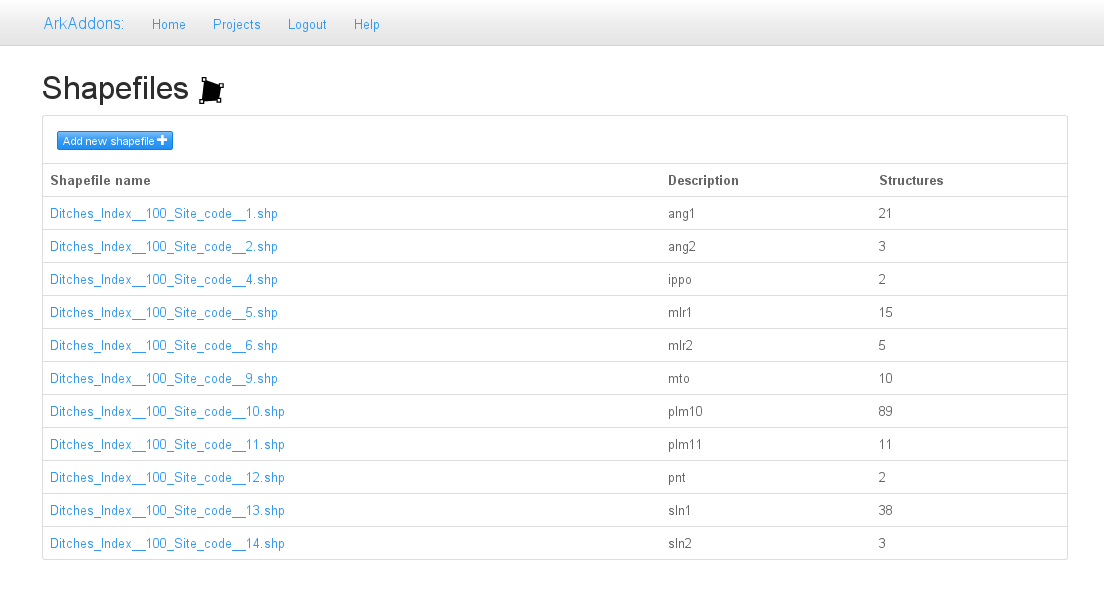
\includegraphics[width=1\textwidth]{img/shp-list}
        \end{frame}

        \begin{frame}{Interfaccia alle funzioni: webGIS}
            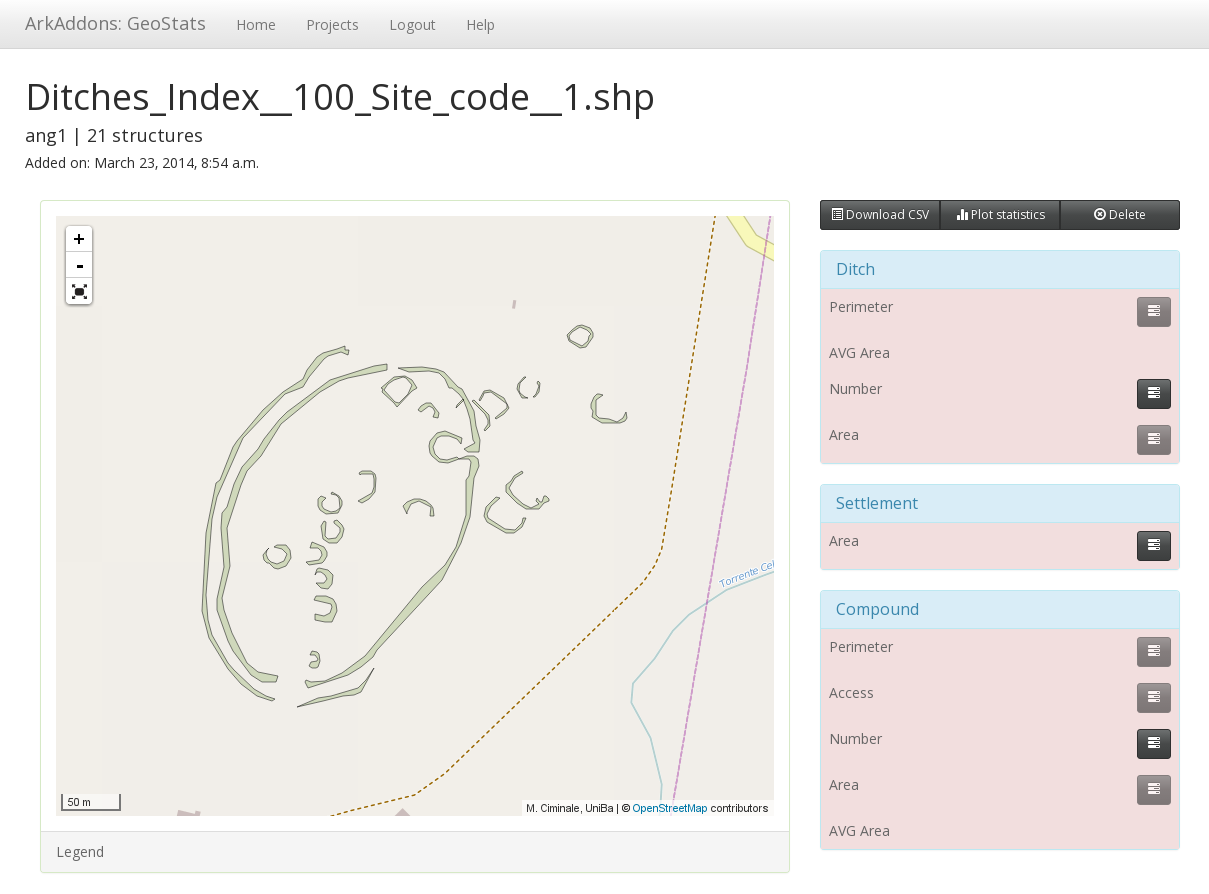
\includegraphics[width=1\textwidth]{img/shp-detail-1}
        \end{frame}

        \begin{frame}{Interfaccia alle funzioni: webGIS}
            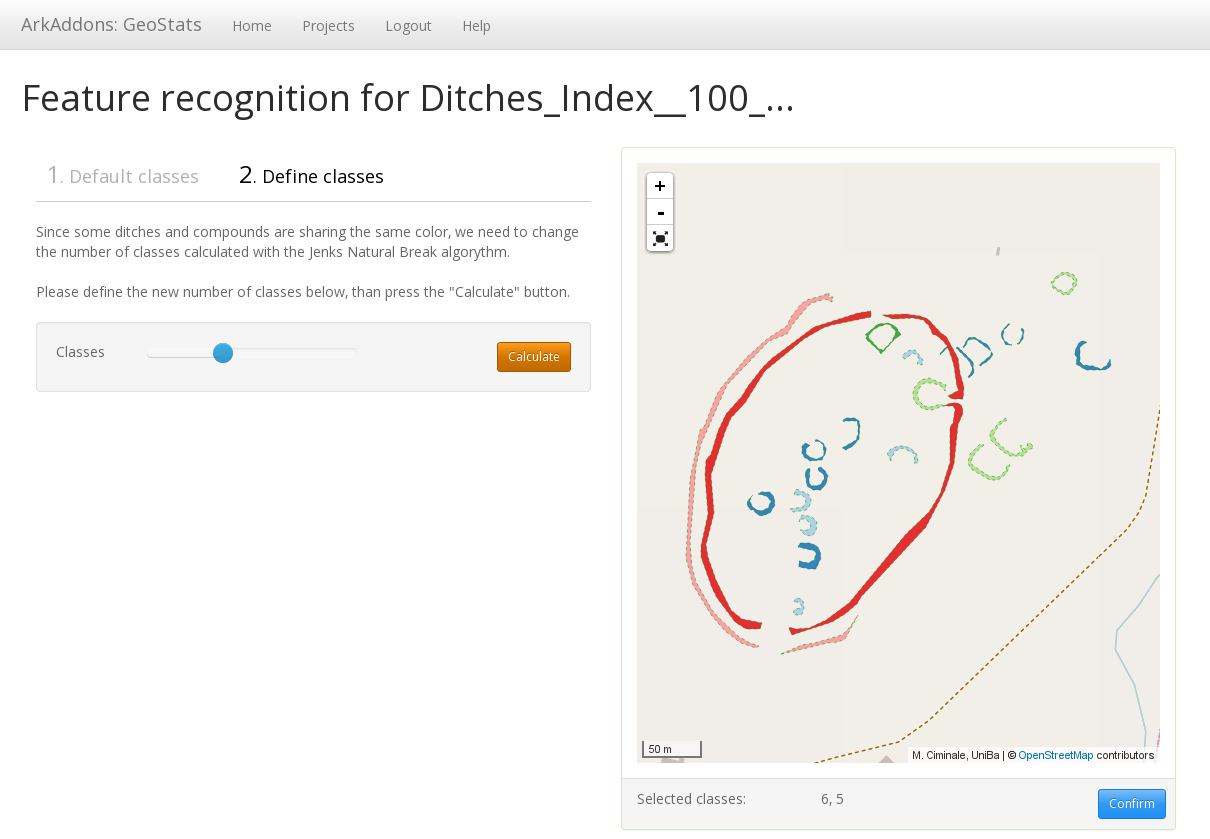
\includegraphics[width=1\textwidth]{img/shp-wizard}
        \end{frame}

        \begin{frame}{Interfaccia alle funzioni: webGIS}
            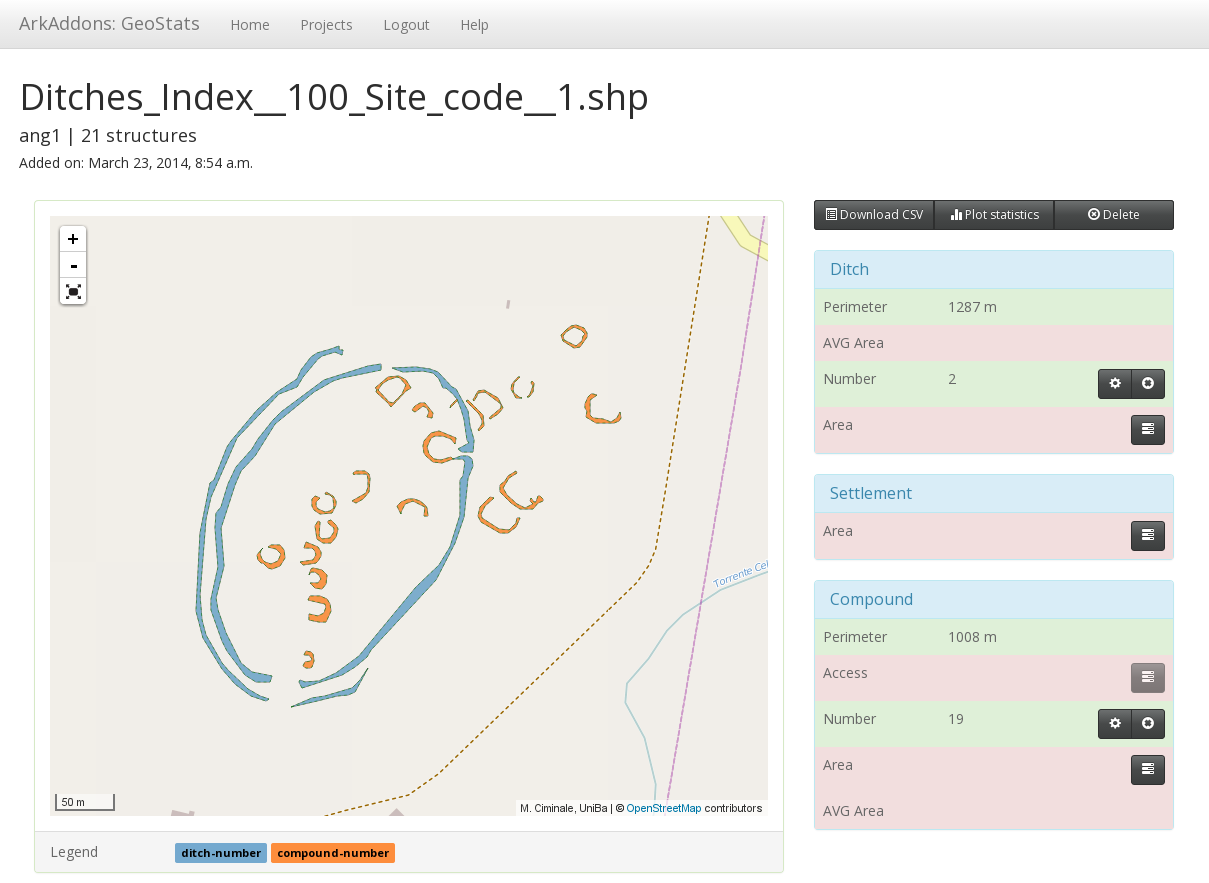
\includegraphics[width=1\textwidth]{img/shp-detail-2}
        \end{frame}

        \begin{frame}{Interfaccia alle funzioni: webGIS}
            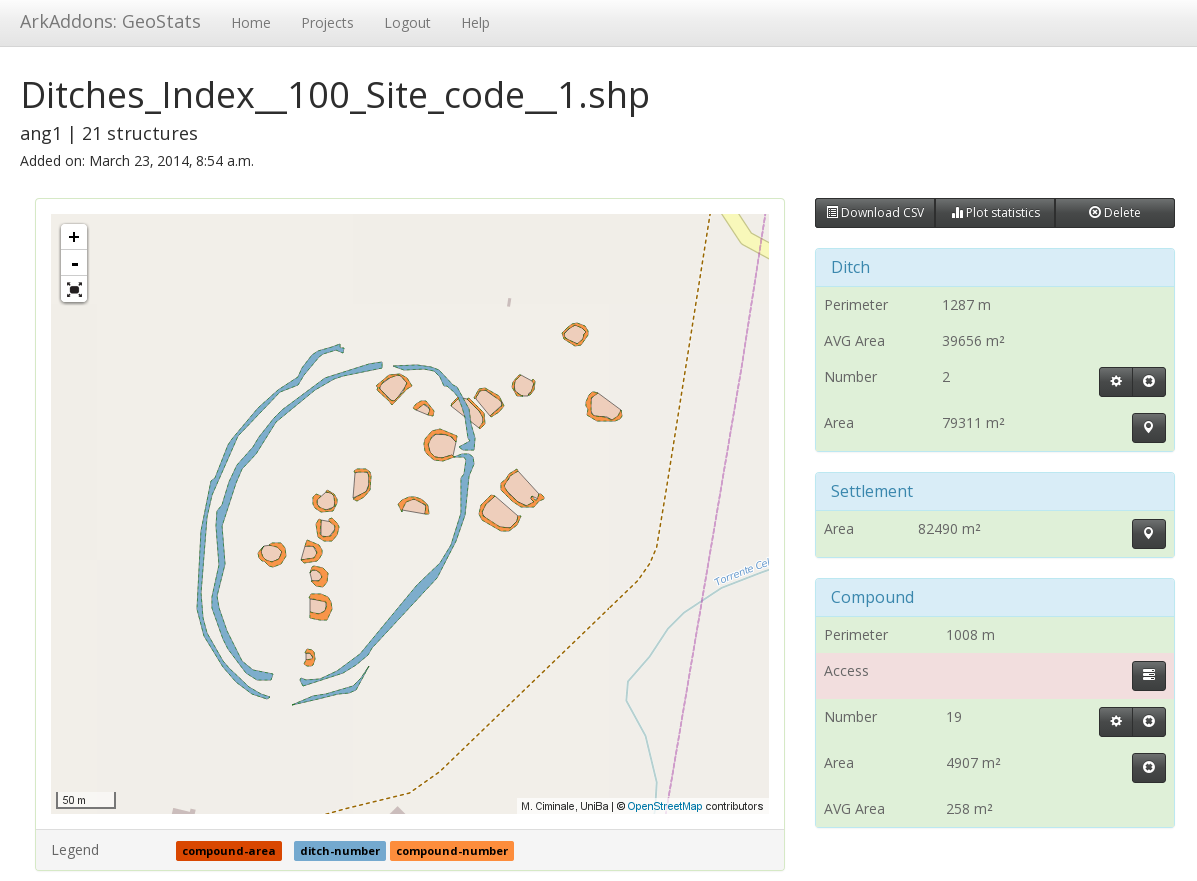
\includegraphics[width=1\textwidth]{img/shp-detail-3}
        \end{frame}

        \begin{frame}{Interfaccia alle funzioni: webGIS}
            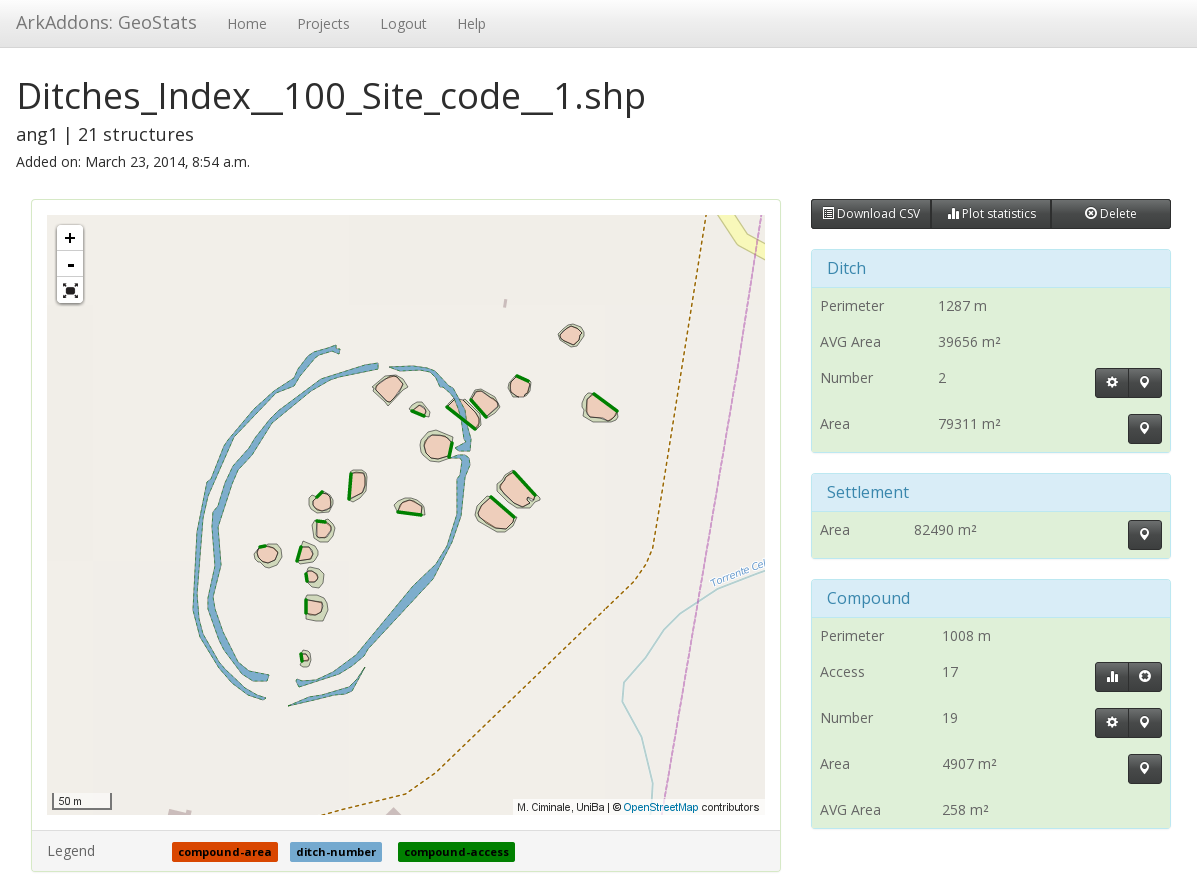
\includegraphics[width=1\textwidth]{img/shp-detail-4}
        \end{frame}

        \begin{frame}{Interfaccia alle funzioni: webGIS}
            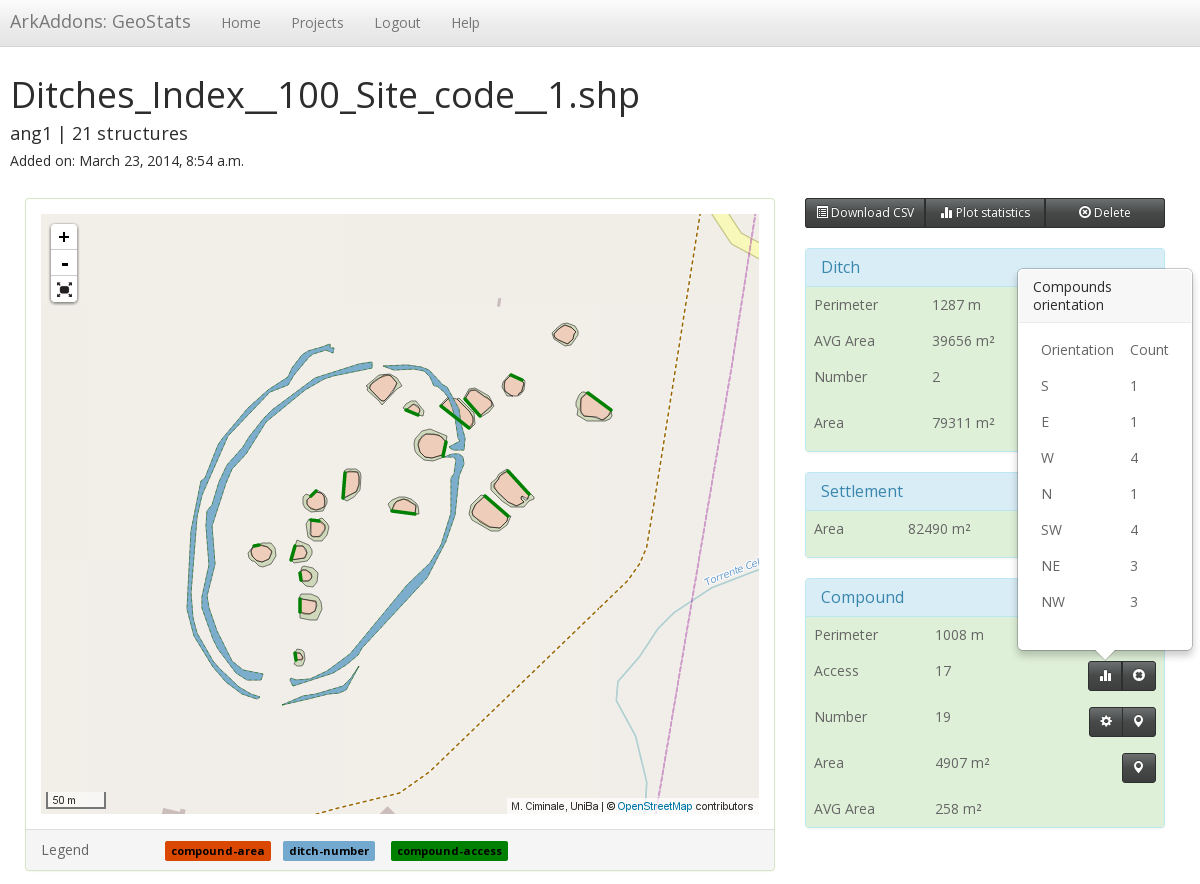
\includegraphics[width=1\textwidth]{img/shp-detail-5}
        \end{frame}

    \section{Statistiche}

        \begin{frame}{Affidabilità: numero di \emph{ditches} e \emph{compounds}}
            \centering
            \begin{tikzpicture}
                \pgfplotstableread{tab/raw/number-comp}{\loadedtable}
\small

\begin{axis}[
    width=1\textwidth,
    height=0.4\textwidth,
    bar width=5pt,
    ybar,
    ymin=0,
    enlarge x limits,
    ylabel=\scriptsize{compounds $(n)$},
    xtick={1,...,11},   % indicates xticks going from 1 to 11
    xticklabels from table={\loadedtable}{set},
    xticklabel style={rotate=45,font=\tiny},
    xticklabel shift=-3pt,
    yticklabel style={font=\tiny},
    legend style={font=\tiny,draw=black!40}
]
    \addplot table[x=id, y=laterza] from \loadedtable;
    \addplot table[x=id, y=current] from \loadedtable;
    \legend{Lat13,current}
\end{axis}

            \end{tikzpicture}

            \begin{tikzpicture}
                \pgfplotstableread{tab/raw/number-ditch}{\loadedtable}
\small

\begin{axis}[
    width=1\textwidth,
    height=0.4\textwidth,
    bar width=5pt,
    ybar,
    ymin=0,
    enlarge x limits,
    xlabel=\tiny{insediamenti},
    xlabel shift=-5pt,
    ylabel=\scriptsize{ditches $(n)$},
    xtick={1,...,11},   % indicates xticks going from 1 to 11
    xticklabels from table={\loadedtable}{set},
    xticklabel style={rotate=45,font=\tiny},
    xticklabel shift=-3pt,
    yticklabel style={font=\tiny},
]
    \addplot table[x=id, y=laterza] from \loadedtable;
    \addplot table[x=id, y=current] from \loadedtable;
\end{axis}

            \end{tikzpicture}
        \end{frame}

        \begin{frame}{Affidabilità: aree e perimetri}
            \centering
            \begin{tikzpicture}
                \pgfplotstableread[col sep=comma]{tab/raw/aree.csv}{\loadedtable}
\small

\begin{axis}[
    width=1\textwidth,
    height=0.4\textwidth,
    bar width=5pt,
    ybar,
    ymin=0,
    enlarge x limits,
    ylabel=\scriptsize{area $(\si{\meter\squared})$},
    xtick={1,...,11},   % indicates xticks going from 1 to 11
    xticklabels from table={\loadedtable}{set},
    xticklabel style={rotate=45,font=\tiny},
    xticklabel shift=-3pt,
    yticklabel style={font=\tiny},
    legend style={font=\tiny,draw=black!40}
]
    \addplot table[x=id, y=laterza] from \loadedtable;
    \addplot table[x=id, y=current] from \loadedtable;
    \legend{Lat13,current}
\end{axis}

            \end{tikzpicture}

            \begin{tikzpicture}
                \pgfplotstableread[col sep=comma]{tab/raw/perim.csv}{\loadedtable}
\small

\begin{axis}[
    width=1\textwidth,
    height=0.4\textwidth,
    bar width=5pt,
    ybar,
    ymin=0,
    enlarge x limits,
    xlabel=\tiny{insediamenti},
    xlabel shift=-5pt,
    ylabel=\scriptsize{perimetro $(m)$},
    xtick={1,...,11},   % indicates xticks going from 1 to 11
    xticklabels from table={\loadedtable}{set},
    xticklabel style={rotate=45,font=\tiny},
    xticklabel shift=-3pt,
    yticklabel style={font=\tiny},
]
    \addplot table[x=id, y=laterza] from \loadedtable;
    \addplot table[x=id, y=current] from \loadedtable;
\end{axis}

            \end{tikzpicture}
        \end{frame}

        \begin{frame}{Affidabilità: aree e perimetri}
            \begin{tikzpicture}
                \pgfplotstableread[col sep=comma]{tab/raw/orient.csv}{\loadedtable}
\small

\begin{axis}[
    width=1\textwidth,
    height=0.45\textwidth,
    bar width=5pt,
    ybar,
    ymin=0,
    enlarge x limits,
    xlabel=\tiny{orientazione dei compounds},
    xlabel shift=-5pt,
    ylabel=\scriptsize{frequenza $(n)$},
    xtick={1,...,8},   % indicates xticks going from 1 to 11
    xticklabels from table={\loadedtable}{orient},
    xticklabel style={rotate=45,font=\tiny},
    xticklabel shift=-3pt,
    yticklabel style={font=\tiny},
    legend style={font=\tiny,legend pos=north west,draw=black!40}
]
    \addplot table[x=id, y=laterza] from \loadedtable;
    \addplot table[x=id, y=current] from \loadedtable;
    \legend{Lat13,current}
\end{axis}

            \end{tikzpicture}
            \pause
            \scriptsize
            \begin{align*}
                H_0 : \sigma^2_1 = \sigma^2_2   &&  s^2 &= \frac{1}{N-1} \sum_{i=1}^N (x_i - \overline{x})^2    &&  F_{\text{cal}} = \frac{s^2_2}{s^2_1} = 1.07\\
                H_a : \sigma^2_1\neq\sigma^2_2  &&  s^2_{1} &= 438.79   &&  F_{\text{cal}} < F_{\text{tab}}\\
                                                &&  s^2_{2} &= 470.84   &&  H_0\text{~verificata}
            \end{align*}
        \end{frame}

    \section{Conclusioni}

        \begin{frame}{Conclusioni}
            \centering
            Dati: 11 insediamenti -- 155 compounds
            \vfill
            \begin{tabular}[c]{ccc}
                \toprule
                &   Metodo standard     &   Metodo proposto\\
                \otoprule
                tempi           &   $\sim2$ mesi            &   $\sim\SI{30}{\minute}$\\\pause
                affidabilità    &   $100\%$                 &   $100\%$\\\pause
                riproducibilità &   parziale                &   completa\\\pause
                software        &   installazione locale    &   internet (webGIS)\\\pause
                costi           &   licenza GIS (\EUR{2850})&   open source: \EUR{0}\\
                \bottomrule
            \end{tabular}
        \end{frame}

        \begin{frame}
            \vfill
            \centering
            \Huge
            Grazie
            \vfill
            \scriptsize
            \begin{quote}
                \centering
                So Long, and Thanks for All the Fish\\
                \attrib{D. Adams}
            \end{quote}
            \vfill
        \end{frame}

\end{document}
